% -----------------------------------------------------------------------------
%                                     HEADER                                    
% -----------------------------------------------------------------------------
\documentclass[a4paper, 10pt]{article}
\usepackage{jheppub}
\usepackage[T1]{fontenc}
\usepackage{colortbl,xcolor,float}
\definecolor{orange}{rgb}{1,0.5,0}
% -----------------------------------------------------------------------------
%                                   COVER PAGE                                  
% -----------------------------------------------------------------------------
\title{{\includegraphics[scale=.4]{logo.eps}}\ The LaTeX report}

\author{Generated by elijahsheridan on 12 September 2020, 15:13:44}

\abstract{
  This report has been generated automatically
  by {\sc MadAnalysis} 5.\\$~$\\ 
  Please cite:\\ 
  \begin{quote}
    \textbf{E.~Conte, B.~Fuks and G.~Serret},\\ 
    \textit{MadAnalysis 5, A User-Friendly
    Framework for Collider Phenomenology},\\ 
    Comput. Phys. Commun. {\bf 184} (2013) 222-256,\\
    arXiv:1206.1599 [hep-ph].\\ 
  \end{quote}
  To contact us:\\ 
  \begin{quote}
    \textbf{http://madanalysis.irmp.ucl.ac.be}\\
    \textbf{ma5team@iphc.cnrs.fr}\\
  \end{quote}
}

% -----------------------------------------------------------------------------
%                                 BEGIN DOCUMENT                                
% -----------------------------------------------------------------------------
\begin{document}
\maketitle
\flushbottom

% -----------------------------------------------------------------------------
%                                 SECTION Setup                                 
% -----------------------------------------------------------------------------
\newpage
\section{ Setup}

\subsection{ Command history}

\texttt{ma5>\# set directory where running "./\-bin/\-ma5"; set lumi; define the signal significance\\
}
\texttt{ }\texttt{ }\texttt{ma5>set main.currentdir = /\-Users/\-elijahsheridan/\-MG5\_aMC\_v2\_6\_5/\-axion\_pheno/\-madgraph\_data \# need to change this directory path --> exit and type "pwd" to get the path\\
}
\texttt{ }\texttt{ }\texttt{ma5>set main.lumi = 40\\
}
\texttt{ }\texttt{ }\texttt{ma5>set main.fom.formula = 5\\
}
\texttt{ }\texttt{ }\texttt{ma5>set main.fom.x = 0.25\\
}
\texttt{ }\texttt{ }\texttt{ma5>\# import samples --> change the path to the LHE file\\
}
\texttt{ }\texttt{ }\texttt{ma5>import /\-Users/\-elijahsheridan/\-MG5\_aMC\_v2\_6\_5/\-axion\_pheno/\-madgraph\_data/\-axion\_signal/\-on\_discovery\_contour/\-ma100MeV\_L1pt8TeV\_deta2.lhe.gz as signal\_1pt8TeVL\\
}
\texttt{ }\texttt{ }\texttt{ma5>import /\-Users/\-elijahsheridan/\-MG5\_aMC\_v2\_6\_5/\-axion\_pheno/\-madgraph\_data/\-axion\_signal/\-on\_discovery\_contour/\-ma100MeV\_L2TeV\_deta2.lhe as signal\_2TeVL\\
}
\texttt{ }\texttt{ }\texttt{ma5>import /\-Users/\-elijahsheridan/\-MG5\_aMC\_v2\_6\_5/\-axion\_pheno/\-madgraph\_data/\-axion\_signal/\-on\_discovery\_contour/\-ma100MeV\_L2pt2TeV\_deta2.lhe.gz as signal\_2pt2TeVL\\
}
\texttt{ }\texttt{ }\texttt{ma5>import /\-Users/\-elijahsheridan/\-MG5\_aMC\_v2\_6\_5/\-axion\_pheno/\-madgraph\_data/\-axion\_signal/\-on\_discovery\_contour/\-ma100MeV\_L2pt4TeV\_deta2.lhe.gz as signal\_2pt4TeVL\\
}
\texttt{ }\texttt{ }\texttt{ma5>import /\-Users/\-elijahsheridan/\-MG5\_aMC\_v2\_6\_5/\-axion\_pheno/\-madgraph\_data/\-diphoton\_double\_isr\_background\_data/\-merged\_lhe/\-diphoton\_double\_isr\_background\_ht\_0\_100\_merged.lhe.gz as bg\_dip\_0\_100\\
}
\texttt{ }\texttt{ }\texttt{ma5>import /\-Users/\-elijahsheridan/\-MG5\_aMC\_v2\_6\_5/\-axion\_pheno/\-madgraph\_data/\-diphoton\_double\_isr\_background\_data/\-merged\_lhe/\-diphoton\_double\_isr\_background\_ht\_100\_200\_merged.lhe.gz as bg\_dip\_100\_200\\
}
\texttt{ }\texttt{ }\texttt{ma5>import /\-Users/\-elijahsheridan/\-MG5\_aMC\_v2\_6\_5/\-axion\_pheno/\-madgraph\_data/\-diphoton\_double\_isr\_background\_data/\-merged\_lhe/\-diphoton\_double\_isr\_background\_ht\_200\_400\_merged.lhe.gz as bg\_dip\_200\_400\\
}
\texttt{ }\texttt{ }\texttt{ma5>import /\-Users/\-elijahsheridan/\-MG5\_aMC\_v2\_6\_5/\-axion\_pheno/\-madgraph\_data/\-diphoton\_double\_isr\_background\_data/\-merged\_lhe/\-diphoton\_double\_isr\_background\_ht\_400\_600\_merged.lhe.gz as bg\_dip\_400\_600\\
}
\texttt{ }\texttt{ }\texttt{ma5>import /\-Users/\-elijahsheridan/\-MG5\_aMC\_v2\_6\_5/\-axion\_pheno/\-madgraph\_data/\-diphoton\_double\_isr\_background\_data/\-merged\_lhe/\-diphoton\_double\_isr\_background\_ht\_600\_800\_merged.lhe.gz as bg\_dip\_600\_800\\
}
\texttt{ }\texttt{ }\texttt{ma5>import /\-Users/\-elijahsheridan/\-MG5\_aMC\_v2\_6\_5/\-axion\_pheno/\-madgraph\_data/\-diphoton\_double\_isr\_background\_data/\-merged\_lhe/\-diphoton\_double\_isr\_background\_ht\_800\_1200\_merged.lhe.gz as bg\_dip\_800\_1200\\
}
\texttt{ }\texttt{ }\texttt{ma5>import /\-Users/\-elijahsheridan/\-MG5\_aMC\_v2\_6\_5/\-axion\_pheno/\-madgraph\_data/\-diphoton\_double\_isr\_background\_data/\-merged\_lhe/\-diphoton\_double\_isr\_background\_ht\_1200\_1600\_merged.lhe.gz as bg\_dip\_1200\_1600\\
}
\texttt{ }\texttt{ }\texttt{ma5>import /\-Users/\-elijahsheridan/\-MG5\_aMC\_v2\_6\_5/\-axion\_pheno/\-madgraph\_data/\-diphoton\_double\_isr\_background\_data/\-merged\_lhe/\-diphoton\_double\_isr\_background\_ht\_1600\_inf\_merged.lhe.gz as bg\_dip\_1600\_inf\\
}
\texttt{ }\texttt{ }\texttt{ma5>import /\-Users/\-elijahsheridan/\-MG5\_aMC\_v2\_6\_5/\-axion\_pheno/\-madgraph\_data/\-vbf\_diphoton\_background\_data/\-merged\_lhe/\-vbf\_diphoton\_background\_ht\_0\_100\_merged.lhe.gz as bg\_vbf\_0\_100\\
}
\texttt{ }\texttt{ }\texttt{ma5>import /\-Users/\-elijahsheridan/\-MG5\_aMC\_v2\_6\_5/\-axion\_pheno/\-madgraph\_data/\-vbf\_diphoton\_background\_data/\-merged\_lhe/\-vbf\_diphoton\_background\_ht\_100\_200\_merged.lhe.gz as bg\_vbf\_100\_200\\
}
\texttt{ }\texttt{ }\texttt{ma5>import /\-Users/\-elijahsheridan/\-MG5\_aMC\_v2\_6\_5/\-axion\_pheno/\-madgraph\_data/\-vbf\_diphoton\_background\_data/\-merged\_lhe/\-vbf\_diphoton\_background\_ht\_200\_400\_merged.lhe.gz as bg\_vbf\_200\_400\\
}
\texttt{ }\texttt{ }\texttt{ma5>import /\-Users/\-elijahsheridan/\-MG5\_aMC\_v2\_6\_5/\-axion\_pheno/\-madgraph\_data/\-vbf\_diphoton\_background\_data/\-merged\_lhe/\-vbf\_diphoton\_background\_ht\_400\_600\_merged.lhe.gz as bg\_vbf\_400\_600\\
}
\texttt{ }\texttt{ }\texttt{ma5>import /\-Users/\-elijahsheridan/\-MG5\_aMC\_v2\_6\_5/\-axion\_pheno/\-madgraph\_data/\-vbf\_diphoton\_background\_data/\-merged\_lhe/\-vbf\_diphoton\_background\_ht\_600\_800\_merged.lhe.gz as bg\_vbf\_600\_800\\
}
\texttt{ }\texttt{ }\texttt{ma5>import /\-Users/\-elijahsheridan/\-MG5\_aMC\_v2\_6\_5/\-axion\_pheno/\-madgraph\_data/\-vbf\_diphoton\_background\_data/\-merged\_lhe/\-vbf\_diphoton\_background\_ht\_800\_1200\_merged.lhe.gz as bg\_vbf\_800\_1200\\
}
\texttt{ }\texttt{ }\texttt{ma5>import /\-Users/\-elijahsheridan/\-MG5\_aMC\_v2\_6\_5/\-axion\_pheno/\-madgraph\_data/\-vbf\_diphoton\_background\_data/\-merged\_lhe/\-vbf\_diphoton\_background\_ht\_1200\_1600\_merged.lhe.gz as bg\_vbf\_1200\_1600\\
}
\texttt{ }\texttt{ }\texttt{ma5>import /\-Users/\-elijahsheridan/\-MG5\_aMC\_v2\_6\_5/\-axion\_pheno/\-madgraph\_data/\-vbf\_diphoton\_background\_data/\-merged\_lhe/\-vbf\_diphoton\_background\_ht\_1600\_inf\_merged.lhe.gz as bg\_vbf\_1600\_inf\\
}
\texttt{ }\texttt{ }\texttt{ma5>\# define bg and signal samples\\
}
\texttt{ }\texttt{ }\texttt{ma5>set signal\_1pt8TeVL.type = signal\\
}
\texttt{ }\texttt{ }\texttt{ma5>set signal\_2TeVL.type = signal\\
}
\texttt{ }\texttt{ }\texttt{ma5>set signal\_2pt2TeVL.type = signal\\
}
\texttt{ }\texttt{ }\texttt{ma5>set signal\_2pt4TeVL.type = signal\\
}
\texttt{ }\texttt{ }\texttt{ma5>set bg\_vbf\_0\_100.type = background\\
}
\texttt{ }\texttt{ }\texttt{ma5>set bg\_vbf\_100\_200.type = background\\
}
\texttt{ }\texttt{ }\texttt{ma5>set bg\_vbf\_200\_400.type  = background\\
}
\texttt{ }\texttt{ }\texttt{ma5>set bg\_vbf\_400\_600.type  = background\\
}
\texttt{ }\texttt{ }\texttt{ma5>set bg\_vbf\_600\_800.type  = background\\
}
\texttt{ }\texttt{ }\texttt{ma5>set bg\_vbf\_800\_1200.type  = background\\
}
\texttt{ }\texttt{ }\texttt{ma5>set bg\_vbf\_1200\_1600.type  = background\\
}
\texttt{ }\texttt{ }\texttt{ma5>set bg\_vbf\_1600\_inf.type = background\\
}
\texttt{ }\texttt{ }\texttt{ma5>set bg\_dip\_0\_100.type = background\\
}
\texttt{ }\texttt{ }\texttt{ma5>set bg\_dip\_100\_200.type = background\\
}
\texttt{ }\texttt{ }\texttt{ma5>set bg\_dip\_200\_400.type = background\\
}
\texttt{ }\texttt{ }\texttt{ma5>set bg\_dip\_400\_600.type = background\\
}
\texttt{ }\texttt{ }\texttt{ma5>set bg\_dip\_600\_800.type = background\\
}
\texttt{ }\texttt{ }\texttt{ma5>set bg\_dip\_800\_1200.type = background\\
}
\texttt{ }\texttt{ }\texttt{ma5>set bg\_dip\_1200\_1600.type = background\\
}
\texttt{ }\texttt{ }\texttt{ma5>set bg\_dip\_1600\_inf.type = background\\
}
\texttt{ }\texttt{ }\texttt{ma5>\# a jet can be from a light quark or b quark\\
}
\texttt{ }\texttt{ }\texttt{ma5>define jets = j\\
}
\texttt{ }\texttt{ }\texttt{ma5>define e = e+ e-\\
}
\texttt{ }\texttt{ }\texttt{ma5>define mu = mu+ mu-\\
}
\texttt{ }\texttt{ }\texttt{ma5>define ta = ta+ ta-\\
}
\texttt{ }\texttt{ }\texttt{ma5>define lept = e mu ta\\
}
\texttt{ }\texttt{ }\texttt{ma5>define ax = 9000005\\
}
\texttt{ }\texttt{ }\texttt{ma5>\# cuts\\
}
\texttt{ }\texttt{ }\texttt{ma5>select ((sdETA(jets[1] jets[2]) > 2.6 or sdETA(jets[1] jets[2]) < -2.6) and M(jets[1] jets[2]) > 750) and (PT(a[1]) > 300 and M(a[1] a[2]) > 500)\\
}
\texttt{ }\texttt{ }\texttt{ma5>\# define which plots to make\\
}
\texttt{ }\texttt{ }\texttt{ma5>plot PT(jets[1])\\
}
\texttt{ }\texttt{ }\texttt{ma5>plot ETA(jets[1])\\
}
\texttt{ }\texttt{ }\texttt{ma5>plot PHI(jets[1])\\
}
\texttt{ }\texttt{ }\texttt{ma5>plot PT(jets[2])\\
}
\texttt{ }\texttt{ }\texttt{ma5>plot ETA(jets[2])\\
}
\texttt{ }\texttt{ }\texttt{ma5>plot PHI(jets[2])\\
}
\texttt{ }\texttt{ }\texttt{ma5>plot DELTAR(jets[1], jets[2])\\
}
\texttt{ }\texttt{ }\texttt{ma5>plot M(jets[1] jets[2])\\
}
\texttt{ }\texttt{ }\texttt{ma5>plot sdETA(jets[1] jets[2])\\
}
\texttt{ }\texttt{ }\texttt{ma5>plot M(a[1] a[2])\\
}
\texttt{ }\texttt{ }\texttt{ma5>plot PT(a[1])\\
}
\texttt{ }\texttt{ }\texttt{ma5>plot PT(a[2])\\
}
\texttt{ }\texttt{ }\texttt{ma5>plot THT\\
}
\texttt{ }\texttt{ }\texttt{ma5>plot MET\\
}
\texttt{ }\texttt{ }\texttt{ma5>plot TET\\
}
\texttt{ }\texttt{ }\texttt{ma5>\#set the plot/\-graph parameters\\
}
\texttt{ }\texttt{ }\texttt{ma5>set selection[2].xmin = 0\\
}
\texttt{ }\texttt{ }\texttt{ma5>set selection[2].xmax = 2000\\
}
\texttt{ }\texttt{ }\texttt{ma5>set selection[2].nbins = 200\\
}
\texttt{ }\texttt{ }\texttt{ma5>set selection[2].rank = PTordering\\
}
\texttt{ }\texttt{ }\texttt{ma5>set selection[2].titleX = "p\_\{T\}[j\_\{1\}] (GeV)"\\
}
\texttt{ }\texttt{ }\texttt{ma5>set selection[3].xmin = -8\\
}
\texttt{ }\texttt{ }\texttt{ma5>set selection[3].xmax = 8\\
}
\texttt{ }\texttt{ }\texttt{ma5>set selection[3].nbins = 160\\
}
\texttt{ }\texttt{ }\texttt{ma5>set selection[3].rank = PTordering\\
}
\texttt{ }\texttt{ }\texttt{ma5>set selection[3].titleX = "\#eta[j\_\{1\}]"\\
}
\texttt{ }\texttt{ }\texttt{ma5>set selection[4].xmin = -3.2\\
}
\texttt{ }\texttt{ }\texttt{ma5>set selection[4].xmax = 3.2\\
}
\texttt{ }\texttt{ }\texttt{ma5>set selection[4].nbins = 64\\
}
\texttt{ }\texttt{ }\texttt{ma5>set selection[4].rank = PTordering\\
}
\texttt{ }\texttt{ }\texttt{ma5>set selection[4].titleX = "\#phi[j\_\{1\}]"\\
}
\texttt{ }\texttt{ }\texttt{ma5>set selection[5].xmin = 0\\
}
\texttt{ }\texttt{ }\texttt{ma5>set selection[5].xmax = 1000\\
}
\texttt{ }\texttt{ }\texttt{ma5>set selection[5].nbins = 100\\
}
\texttt{ }\texttt{ }\texttt{ma5>set selection[5].rank = PTordering\\
}
\texttt{ }\texttt{ }\texttt{ma5>set selection[5].titleX = "p\_\{T\}[j\_\{2\}] (GeV)"\\
}
\texttt{ }\texttt{ }\texttt{ma5>set selection[6].xmin = -8\\
}
\texttt{ }\texttt{ }\texttt{ma5>set selection[6].xmax = 8\\
}
\texttt{ }\texttt{ }\texttt{ma5>set selection[6].nbins = 160\\
}
\texttt{ }\texttt{ }\texttt{ma5>set selection[6].rank = PTordering\\
}
\texttt{ }\texttt{ }\texttt{ma5>set selection[6].titleX = "\#eta[j\_\{2\}]"\\
}
\texttt{ }\texttt{ }\texttt{ma5>set selection[7].xmin = -3.2\\
}
\texttt{ }\texttt{ }\texttt{ma5>set selection[7].xmax = 3.2\\
}
\texttt{ }\texttt{ }\texttt{ma5>set selection[7].nbins = 64\\
}
\texttt{ }\texttt{ }\texttt{ma5>set selection[7].rank = PTordering\\
}
\texttt{ }\texttt{ }\texttt{ma5>set selection[7].titleX = "\#phi[j\_\{2\}]"\\
}
\texttt{ }\texttt{ }\texttt{ma5>set selection[8].xmin = 0\\
}
\texttt{ }\texttt{ }\texttt{ma5>set selection[8].xmax = 15\\
}
\texttt{ }\texttt{ }\texttt{ma5>set selection[8].nbins = 75\\
}
\texttt{ }\texttt{ }\texttt{ma5>set selection[8].rank = PTordering\\
}
\texttt{ }\texttt{ }\texttt{ma5>set selection[8].titleX = "\#DeltaR[j\_\{1\},j\_\{2\}]"\\
}
\texttt{ }\texttt{ }\texttt{ma5>set selection[9].xmin = 750\\
}
\texttt{ }\texttt{ }\texttt{ma5>set selection[9].xmax = 8000\\
}
\texttt{ }\texttt{ }\texttt{ma5>set selection[9].nbins = 160\\
}
\texttt{ }\texttt{ }\texttt{ma5>set selection[9].rank = PTordering\\
}
\texttt{ }\texttt{ }\texttt{ma5>set selection[9].titleX = "M[j\_\{1\},j\_\{2\}] (GeV)"\\
}
\texttt{ }\texttt{ }\texttt{ma5>set selection[10].xmin = 2.6\\
}
\texttt{ }\texttt{ }\texttt{ma5>set selection[10].xmax = 15\\
}
\texttt{ }\texttt{ }\texttt{ma5>set selection[10].titleX = "\#Delta\#eta(j\_\{1\},j\_\{2\})"\\
}
\texttt{ }\texttt{ }\texttt{ma5>set selection[11].xmin = 500\\
}
\texttt{ }\texttt{ }\texttt{ma5>set selection[11].xmax = 4000\\
}
\texttt{ }\texttt{ }\texttt{ma5>set selection[11].nbins = 400\\
}
\texttt{ }\texttt{ }\texttt{ma5>set selection[11].rank = PTordering\\
}
\texttt{ }\texttt{ }\texttt{ma5>set selection[11].titleX = "M[a\_\{1\},a\_\{2\}] (GeV)"\\
}
\texttt{ }\texttt{ }\texttt{ma5>set selection[12].xmin = 300\\
}
\texttt{ }\texttt{ }\texttt{ma5>set selection[12].xmax = 2000\\
}
\texttt{ }\texttt{ }\texttt{ma5>set selection[12].nbins = 80\\
}
\texttt{ }\texttt{ }\texttt{ma5>set selection[12].rank = PTordering\\
}
\texttt{ }\texttt{ }\texttt{ma5>set selection[12].titleX = "p\_\{T\}[a\_\{1\}]"\\
}
\texttt{ }\texttt{ }\texttt{ma5>set selection[13].xmin = 0\\
}
\texttt{ }\texttt{ }\texttt{ma5>set selection[13].xmax = 2000\\
}
\texttt{ }\texttt{ }\texttt{ma5>set selection[13].nbins = 400\\
}
\texttt{ }\texttt{ }\texttt{ma5>set selection[13].rank = PTordering\\
}
\texttt{ }\texttt{ }\texttt{ma5>set selection[13].titleX = "p\_\{T\}[a\_\{2\}] (GeV)"\\
}
\texttt{ }\texttt{ }\texttt{ma5>set selection[14].xmin = 0\\
}
\texttt{ }\texttt{ }\texttt{ma5>set selection[14].xmax = 4000\\
}
\texttt{ }\texttt{ }\texttt{ma5>set selection[14].nbins = 80\\
}
\texttt{ }\texttt{ }\texttt{ma5>set selection[14].rank = PTordering\\
}
\texttt{ }\texttt{ }\texttt{ma5>set selection[14].titleX = "THT"\\
}
\texttt{ }\texttt{ }\texttt{ma5>set selection[15].xmin = 0\\
}
\texttt{ }\texttt{ }\texttt{ma5>set selection[15].xmax = 1000\\
}
\texttt{ }\texttt{ }\texttt{ma5>set selection[15].nbins = 200\\
}
\texttt{ }\texttt{ }\texttt{ma5>set selection[15].rank = PTordering\\
}
\texttt{ }\texttt{ }\texttt{ma5>set selection[15].titleX = "MET"\\
}
\texttt{ }\texttt{ }\texttt{ma5>set selection[16].xmin = 0\\
}
\texttt{ }\texttt{ }\texttt{ma5>set selection[16].xmax = 8000\\
}
\texttt{ }\texttt{ }\texttt{ma5>set selection[16].nbins = 80\\
}
\texttt{ }\texttt{ }\texttt{ma5>set selection[16].rank = PTordering\\
}
\texttt{ }\texttt{ }\texttt{ma5>set selection[16].titleX = "TET"\\
}
\texttt{ }\texttt{ }\texttt{ma5>submit ma100MeV\_L1pt8-2pt4TeV\_deta2pt6s\\
}
\texttt{ }\texttt{ }\subsection{ Configuration}

\begin{itemize}
  \item MadAnalysis version 1.6.33 (2017/\-11/\-20).
   \item Histograms given for an integrated luminosity of \textcolor{blue}{40.0}\textcolor{blue}{ fb}$^{\textcolor{blue}{-1}}$\textcolor{blue}{.}
\textcolor{blue}{}
\end{itemize}
% -----------------------------------------------------------------------------
%                                SECTION Datasets                               
% -----------------------------------------------------------------------------
\newpage
\section{ Datasets}

\subsection{ signal\_1pt8tevl}

\begin{itemize}
  \item Samples stored in the directory: \textcolor{blue}{/\-Users/\-elijahsheridan/\-MG5\_aMC\_v2\_6\_5/\-axion\_pheno/\-post\_optimization\_studies/\-mad\_analyses} .
   \item Sample consisting of: \textcolor{blue}{signal}  events.
   \item Generated events: \textcolor{blue}{100000 }  events.
   \item Normalization to the luminosity: \textcolor{blue}{176}\textcolor{blue}{ +/\-- }\textcolor{blue}{1 }  events.
   \item Ratio (event weight): \textcolor{blue}{0.0018 } .  
 
\end{itemize}
\begin{table}[H]
  \begin{center}
    \begin{tabular}{|m{55.0mm}|m{25.0mm}|m{30.0mm}|m{30.0mm}|}
      \hline
      {\cellcolor{yellow}         Path to the event file}& {\cellcolor{yellow}         Nr. of events}& {\cellcolor{yellow}         Cross section (pb)}& {\cellcolor{yellow}         Negative wgts (\%)}\\
      \hline
      {\cellcolor{white}          /\-Users/\-elijahsheridan/\-MG5\_aMC\_v2\_6\_5/\-axion\_pheno/\-madgraph\_data/\-axion\_signal/\-on\_discovery\_contour/\-ma100MeV\_L1pt8TeV\_deta2.lhe.gz}& {\cellcolor{white}          100000}& {\cellcolor{white}          0.00442 @ 0.095\%}& {\cellcolor{white}          0.0}\\
\hline
    \end{tabular}
  \end{center}
\end{table}

\subsection{ signal\_2tevl}

\begin{itemize}
  \item Samples stored in the directory: \textcolor{blue}{/\-Users/\-elijahsheridan/\-MG5\_aMC\_v2\_6\_5/\-axion\_pheno/\-post\_optimization\_studies/\-mad\_analyses} .
   \item Sample consisting of: \textcolor{blue}{signal}  events.
   \item Generated events: \textcolor{blue}{100000 }  events.
   \item Normalization to the luminosity: \textcolor{blue}{106}\textcolor{blue}{ +/\-- }\textcolor{blue}{1 }  events.
   \item Ratio (event weight): \textcolor{blue}{0.0011 } .  
 
\end{itemize}
\begin{table}[H]
  \begin{center}
    \begin{tabular}{|m{55.0mm}|m{25.0mm}|m{30.0mm}|m{30.0mm}|}
      \hline
      {\cellcolor{yellow}         Path to the event file}& {\cellcolor{yellow}         Nr. of events}& {\cellcolor{yellow}         Cross section (pb)}& {\cellcolor{yellow}         Negative wgts (\%)}\\
      \hline
      {\cellcolor{white}          /\-Users/\-elijahsheridan/\-MG5\_aMC\_v2\_6\_5/\-axion\_pheno/\-madgraph\_data/\-axion\_signal/\-on\_discovery\_contour/\-ma100MeV\_L2TeV\_deta2.lhe}& {\cellcolor{white}          100000}& {\cellcolor{white}          0.00267 @ 0.14\%}& {\cellcolor{white}          0.0}\\
\hline
    \end{tabular}
  \end{center}
\end{table}

\subsection{ signal\_2pt2tevl}

\begin{itemize}
  \item Samples stored in the directory: \textcolor{blue}{/\-Users/\-elijahsheridan/\-MG5\_aMC\_v2\_6\_5/\-axion\_pheno/\-post\_optimization\_studies/\-mad\_analyses} .
   \item Sample consisting of: \textcolor{blue}{signal}  events.
   \item Generated events: \textcolor{blue}{100000 }  events.
   \item Normalization to the luminosity: \textcolor{blue}{69}\textcolor{blue}{ +/\-- }\textcolor{blue}{1 }  events.
   \item Ratio (event weight): \textcolor{blue}{0.00069 } .  
 
\end{itemize}
\begin{table}[H]
  \begin{center}
    \begin{tabular}{|m{55.0mm}|m{25.0mm}|m{30.0mm}|m{30.0mm}|}
      \hline
      {\cellcolor{yellow}         Path to the event file}& {\cellcolor{yellow}         Nr. of events}& {\cellcolor{yellow}         Cross section (pb)}& {\cellcolor{yellow}         Negative wgts (\%)}\\
      \hline
      {\cellcolor{white}          /\-Users/\-elijahsheridan/\-MG5\_aMC\_v2\_6\_5/\-axion\_pheno/\-madgraph\_data/\-axion\_signal/\-on\_discovery\_contour/\-ma100MeV\_L2pt2TeV\_deta2.lhe.gz}& {\cellcolor{white}          100000}& {\cellcolor{white}          0.00174 @ 0.094\%}& {\cellcolor{white}          0.0}\\
\hline
    \end{tabular}
  \end{center}
\end{table}

\subsection{ signal\_2pt4tevl}

\begin{itemize}
  \item Samples stored in the directory: \textcolor{blue}{/\-Users/\-elijahsheridan/\-MG5\_aMC\_v2\_6\_5/\-axion\_pheno/\-post\_optimization\_studies/\-mad\_analyses} .
   \item Sample consisting of: \textcolor{blue}{signal}  events.
   \item Generated events: \textcolor{blue}{100000 }  events.
   \item Normalization to the luminosity: \textcolor{blue}{47}\textcolor{blue}{ +/\-- }\textcolor{blue}{1 }  events.
   \item Ratio (event weight): \textcolor{blue}{0.00047 } .  
 
\end{itemize}
\begin{table}[H]
  \begin{center}
    \begin{tabular}{|m{55.0mm}|m{25.0mm}|m{30.0mm}|m{30.0mm}|}
      \hline
      {\cellcolor{yellow}         Path to the event file}& {\cellcolor{yellow}         Nr. of events}& {\cellcolor{yellow}         Cross section (pb)}& {\cellcolor{yellow}         Negative wgts (\%)}\\
      \hline
      {\cellcolor{white}          /\-Users/\-elijahsheridan/\-MG5\_aMC\_v2\_6\_5/\-axion\_pheno/\-madgraph\_data/\-axion\_signal/\-on\_discovery\_contour/\-ma100MeV\_L2pt4TeV\_deta2.lhe.gz}& {\cellcolor{white}          100000}& {\cellcolor{white}          0.00119 @ 0.097\%}& {\cellcolor{white}          0.0}\\
\hline
    \end{tabular}
  \end{center}
\end{table}

\subsection{ bg\_dip\_0\_100}

\begin{itemize}
  \item Samples stored in the directory: \textcolor{blue}{/\-Users/\-elijahsheridan/\-MG5\_aMC\_v2\_6\_5/\-axion\_pheno/\-post\_optimization\_studies/\-mad\_analyses} .
   \item Sample consisting of: \textcolor{blue}{background}  events.
   \item Generated events: \textcolor{blue}{1040000 }  events.
   \item Normalization to the luminosity: \textcolor{blue}{2710847}\textcolor{blue}{ +/\-- }\textcolor{blue}{4614 }  events.
   \item\textcolor{red}{Ratio (event weight): }\textcolor{red}{2.6 }\textcolor{red}{ - warning: please generate more events (weight larger than 1)!}
\textcolor{red}{}
\end{itemize}
\begin{table}[H]
  \begin{center}
    \begin{tabular}{|m{55.0mm}|m{25.0mm}|m{30.0mm}|m{30.0mm}|}
      \hline
      {\cellcolor{yellow}         Path to the event file}& {\cellcolor{yellow}         Nr. of events}& {\cellcolor{yellow}         Cross section (pb)}& {\cellcolor{yellow}         Negative wgts (\%)}\\
      \hline
      {\cellcolor{white}          /\-Users/\-elijahsheridan/\-MG5\_aMC\_v2\_6\_5/\-axion\_pheno/\-madgraph\_data/\-diphoton\_double\_isr\_background\_data/\-merged\_lhe/\-diphoton\_double\_isr\_background\_ht\_0\_100\_merged.lhe.gz}& {\cellcolor{white}          1040000}& {\cellcolor{white}          67.8 @ 0.17\%}& {\cellcolor{white}          0.0}\\
\hline
    \end{tabular}
  \end{center}
\end{table}

\subsection{ bg\_dip\_100\_200}

\begin{itemize}
  \item Samples stored in the directory: \textcolor{blue}{/\-Users/\-elijahsheridan/\-MG5\_aMC\_v2\_6\_5/\-axion\_pheno/\-post\_optimization\_studies/\-mad\_analyses} .
   \item Sample consisting of: \textcolor{blue}{background}  events.
   \item Generated events: \textcolor{blue}{1040000 }  events.
   \item Normalization to the luminosity: \textcolor{blue}{1095362}\textcolor{blue}{ +/\-- }\textcolor{blue}{1528 }  events.
   \item\textcolor{red}{Ratio (event weight): }\textcolor{red}{1.1 }\textcolor{red}{ - warning: please generate more events (weight larger than 1)!}
\textcolor{red}{}
\end{itemize}
\begin{table}[H]
  \begin{center}
    \begin{tabular}{|m{55.0mm}|m{25.0mm}|m{30.0mm}|m{30.0mm}|}
      \hline
      {\cellcolor{yellow}         Path to the event file}& {\cellcolor{yellow}         Nr. of events}& {\cellcolor{yellow}         Cross section (pb)}& {\cellcolor{yellow}         Negative wgts (\%)}\\
      \hline
      {\cellcolor{white}          /\-Users/\-elijahsheridan/\-MG5\_aMC\_v2\_6\_5/\-axion\_pheno/\-madgraph\_data/\-diphoton\_double\_isr\_background\_data/\-merged\_lhe/\-diphoton\_double\_isr\_background\_ht\_100\_200\_merged.lhe.gz}& {\cellcolor{white}          1040000}& {\cellcolor{white}          27.4 @ 0.14\%}& {\cellcolor{white}          0.0}\\
\hline
    \end{tabular}
  \end{center}
\end{table}

\subsection{ bg\_dip\_200\_400}

\begin{itemize}
  \item Samples stored in the directory: \textcolor{blue}{/\-Users/\-elijahsheridan/\-MG5\_aMC\_v2\_6\_5/\-axion\_pheno/\-post\_optimization\_studies/\-mad\_analyses} .
   \item Sample consisting of: \textcolor{blue}{background}  events.
   \item Generated events: \textcolor{blue}{1040000 }  events.
   \item Normalization to the luminosity: \textcolor{blue}{239548}\textcolor{blue}{ +/\-- }\textcolor{blue}{414 }  events.
   \item Ratio (event weight): \textcolor{blue}{0.23 } .  
 
\end{itemize}
\begin{table}[H]
  \begin{center}
    \begin{tabular}{|m{55.0mm}|m{25.0mm}|m{30.0mm}|m{30.0mm}|}
      \hline
      {\cellcolor{yellow}         Path to the event file}& {\cellcolor{yellow}         Nr. of events}& {\cellcolor{yellow}         Cross section (pb)}& {\cellcolor{yellow}         Negative wgts (\%)}\\
      \hline
      {\cellcolor{white}          /\-Users/\-elijahsheridan/\-MG5\_aMC\_v2\_6\_5/\-axion\_pheno/\-madgraph\_data/\-diphoton\_double\_isr\_background\_data/\-merged\_lhe/\-diphoton\_double\_isr\_background\_ht\_200\_400\_merged.lhe.gz}& {\cellcolor{white}          1040000}& {\cellcolor{white}          5.99 @ 0.17\%}& {\cellcolor{white}          0.0}\\
\hline
    \end{tabular}
  \end{center}
\end{table}

\subsection{ bg\_dip\_400\_600}

\begin{itemize}
  \item Samples stored in the directory: \textcolor{blue}{/\-Users/\-elijahsheridan/\-MG5\_aMC\_v2\_6\_5/\-axion\_pheno/\-post\_optimization\_studies/\-mad\_analyses} .
   \item Sample consisting of: \textcolor{blue}{background}  events.
   \item Generated events: \textcolor{blue}{1040000 }  events.
   \item Normalization to the luminosity: \textcolor{blue}{28798}\textcolor{blue}{ +/\-- }\textcolor{blue}{53 }  events.
   \item Ratio (event weight): \textcolor{blue}{0.028 } .  
 
\end{itemize}
\begin{table}[H]
  \begin{center}
    \begin{tabular}{|m{55.0mm}|m{25.0mm}|m{30.0mm}|m{30.0mm}|}
      \hline
      {\cellcolor{yellow}         Path to the event file}& {\cellcolor{yellow}         Nr. of events}& {\cellcolor{yellow}         Cross section (pb)}& {\cellcolor{yellow}         Negative wgts (\%)}\\
      \hline
      {\cellcolor{white}          /\-Users/\-elijahsheridan/\-MG5\_aMC\_v2\_6\_5/\-axion\_pheno/\-madgraph\_data/\-diphoton\_double\_isr\_background\_data/\-merged\_lhe/\-diphoton\_double\_isr\_background\_ht\_400\_600\_merged.lhe.gz}& {\cellcolor{white}          1040000}& {\cellcolor{white}          0.72 @ 0.18\%}& {\cellcolor{white}          0.0}\\
\hline
    \end{tabular}
  \end{center}
\end{table}

\subsection{ bg\_dip\_600\_800}

\begin{itemize}
  \item Samples stored in the directory: \textcolor{blue}{/\-Users/\-elijahsheridan/\-MG5\_aMC\_v2\_6\_5/\-axion\_pheno/\-post\_optimization\_studies/\-mad\_analyses} .
   \item Sample consisting of: \textcolor{blue}{background}  events.
   \item Generated events: \textcolor{blue}{662009 }  events.
   \item Normalization to the luminosity: \textcolor{blue}{6674}\textcolor{blue}{ +/\-- }\textcolor{blue}{28 }  events.
   \item Ratio (event weight): \textcolor{blue}{0.01 } .  
 
\end{itemize}
\begin{table}[H]
  \begin{center}
    \begin{tabular}{|m{55.0mm}|m{25.0mm}|m{30.0mm}|m{30.0mm}|}
      \hline
      {\cellcolor{yellow}         Path to the event file}& {\cellcolor{yellow}         Nr. of events}& {\cellcolor{yellow}         Cross section (pb)}& {\cellcolor{yellow}         Negative wgts (\%)}\\
      \hline
      {\cellcolor{white}          /\-Users/\-elijahsheridan/\-MG5\_aMC\_v2\_6\_5/\-axion\_pheno/\-madgraph\_data/\-diphoton\_double\_isr\_background\_data/\-merged\_lhe/\-diphoton\_double\_isr\_background\_ht\_600\_800\_merged.lhe.gz}& {\cellcolor{white}          662009}& {\cellcolor{white}          0.167 @ 0.41\%}& {\cellcolor{white}          0.0}\\
\hline
    \end{tabular}
  \end{center}
\end{table}

\subsection{ bg\_dip\_800\_1200}

\begin{itemize}
  \item Samples stored in the directory: \textcolor{blue}{/\-Users/\-elijahsheridan/\-MG5\_aMC\_v2\_6\_5/\-axion\_pheno/\-post\_optimization\_studies/\-mad\_analyses} .
   \item Sample consisting of: \textcolor{blue}{background}  events.
   \item Generated events: \textcolor{blue}{1040000 }  events.
   \item Normalization to the luminosity: \textcolor{blue}{2942}\textcolor{blue}{ +/\-- }\textcolor{blue}{6 }  events.
   \item Ratio (event weight): \textcolor{blue}{0.0028 } .  
 
\end{itemize}
\begin{table}[H]
  \begin{center}
    \begin{tabular}{|m{55.0mm}|m{25.0mm}|m{30.0mm}|m{30.0mm}|}
      \hline
      {\cellcolor{yellow}         Path to the event file}& {\cellcolor{yellow}         Nr. of events}& {\cellcolor{yellow}         Cross section (pb)}& {\cellcolor{yellow}         Negative wgts (\%)}\\
      \hline
      {\cellcolor{white}          /\-Users/\-elijahsheridan/\-MG5\_aMC\_v2\_6\_5/\-axion\_pheno/\-madgraph\_data/\-diphoton\_double\_isr\_background\_data/\-merged\_lhe/\-diphoton\_double\_isr\_background\_ht\_800\_1200\_merged.lhe.gz}& {\cellcolor{white}          1040000}& {\cellcolor{white}          0.0736 @ 0.17\%}& {\cellcolor{white}          0.0}\\
\hline
    \end{tabular}
  \end{center}
\end{table}

\subsection{ bg\_dip\_1200\_1600}

\begin{itemize}
  \item Samples stored in the directory: \textcolor{blue}{/\-Users/\-elijahsheridan/\-MG5\_aMC\_v2\_6\_5/\-axion\_pheno/\-post\_optimization\_studies/\-mad\_analyses} .
   \item Sample consisting of: \textcolor{blue}{background}  events.
   \item Generated events: \textcolor{blue}{337115 }  events.
   \item Normalization to the luminosity: \textcolor{blue}{513}\textcolor{blue}{ +/\-- }\textcolor{blue}{3 }  events.
   \item Ratio (event weight): \textcolor{blue}{0.0015 } .  
 
\end{itemize}
\begin{table}[H]
  \begin{center}
    \begin{tabular}{|m{55.0mm}|m{25.0mm}|m{30.0mm}|m{30.0mm}|}
      \hline
      {\cellcolor{yellow}         Path to the event file}& {\cellcolor{yellow}         Nr. of events}& {\cellcolor{yellow}         Cross section (pb)}& {\cellcolor{yellow}         Negative wgts (\%)}\\
      \hline
      {\cellcolor{white}          /\-Users/\-elijahsheridan/\-MG5\_aMC\_v2\_6\_5/\-axion\_pheno/\-madgraph\_data/\-diphoton\_double\_isr\_background\_data/\-merged\_lhe/\-diphoton\_double\_isr\_background\_ht\_1200\_1600\_merged.lhe.gz}& {\cellcolor{white}          337115}& {\cellcolor{white}          0.0128 @ 0.51\%}& {\cellcolor{white}          0.0}\\
\hline
    \end{tabular}
  \end{center}
\end{table}

\subsection{ bg\_dip\_1600\_inf}

\begin{itemize}
  \item Samples stored in the directory: \textcolor{blue}{/\-Users/\-elijahsheridan/\-MG5\_aMC\_v2\_6\_5/\-axion\_pheno/\-post\_optimization\_studies/\-mad\_analyses} .
   \item Sample consisting of: \textcolor{blue}{background}  events.
   \item Generated events: \textcolor{blue}{1040000 }  events.
   \item Normalization to the luminosity: \textcolor{blue}{187}\textcolor{blue}{ +/\-- }\textcolor{blue}{1 }  events.
   \item Ratio (event weight): \textcolor{blue}{0.00018 } .  
 
\end{itemize}
\begin{table}[H]
  \begin{center}
    \begin{tabular}{|m{55.0mm}|m{25.0mm}|m{30.0mm}|m{30.0mm}|}
      \hline
      {\cellcolor{yellow}         Path to the event file}& {\cellcolor{yellow}         Nr. of events}& {\cellcolor{yellow}         Cross section (pb)}& {\cellcolor{yellow}         Negative wgts (\%)}\\
      \hline
      {\cellcolor{white}          /\-Users/\-elijahsheridan/\-MG5\_aMC\_v2\_6\_5/\-axion\_pheno/\-madgraph\_data/\-diphoton\_double\_isr\_background\_data/\-merged\_lhe/\-diphoton\_double\_isr\_background\_ht\_1600\_inf\_merged.lhe.gz}& {\cellcolor{white}          1040000}& {\cellcolor{white}          0.00469 @ 0.15\%}& {\cellcolor{white}          0.0}\\
\hline
    \end{tabular}
  \end{center}
\end{table}

\subsection{ bg\_vbf\_0\_100}

\begin{itemize}
  \item Samples stored in the directory: \textcolor{blue}{/\-Users/\-elijahsheridan/\-MG5\_aMC\_v2\_6\_5/\-axion\_pheno/\-post\_optimization\_studies/\-mad\_analyses} .
   \item Sample consisting of: \textcolor{blue}{background}  events.
   \item Generated events: \textcolor{blue}{1000000 }  events.
   \item Normalization to the luminosity: \textcolor{blue}{12150}\textcolor{blue}{ +/\-- }\textcolor{blue}{24 }  events.
   \item Ratio (event weight): \textcolor{blue}{0.012 } .  
 
\end{itemize}
\begin{table}[H]
  \begin{center}
    \begin{tabular}{|m{55.0mm}|m{25.0mm}|m{30.0mm}|m{30.0mm}|}
      \hline
      {\cellcolor{yellow}         Path to the event file}& {\cellcolor{yellow}         Nr. of events}& {\cellcolor{yellow}         Cross section (pb)}& {\cellcolor{yellow}         Negative wgts (\%)}\\
      \hline
      {\cellcolor{white}          /\-Users/\-elijahsheridan/\-MG5\_aMC\_v2\_6\_5/\-axion\_pheno/\-madgraph\_data/\-vbf\_diphoton\_background\_data/\-merged\_lhe/\-vbf\_diphoton\_background\_ht\_0\_100\_merged.lhe.gz}& {\cellcolor{white}          1000000}& {\cellcolor{white}          0.304 @ 0.19\%}& {\cellcolor{white}          0.0}\\
\hline
    \end{tabular}
  \end{center}
\end{table}

\subsection{ bg\_vbf\_100\_200}

\begin{itemize}
  \item Samples stored in the directory: \textcolor{blue}{/\-Users/\-elijahsheridan/\-MG5\_aMC\_v2\_6\_5/\-axion\_pheno/\-post\_optimization\_studies/\-mad\_analyses} .
   \item Sample consisting of: \textcolor{blue}{background}  events.
   \item Generated events: \textcolor{blue}{965662 }  events.
   \item Normalization to the luminosity: \textcolor{blue}{9695}\textcolor{blue}{ +/\-- }\textcolor{blue}{17 }  events.
   \item Ratio (event weight): \textcolor{blue}{0.01 } .  
 
\end{itemize}
\begin{table}[H]
  \begin{center}
    \begin{tabular}{|m{55.0mm}|m{25.0mm}|m{30.0mm}|m{30.0mm}|}
      \hline
      {\cellcolor{yellow}         Path to the event file}& {\cellcolor{yellow}         Nr. of events}& {\cellcolor{yellow}         Cross section (pb)}& {\cellcolor{yellow}         Negative wgts (\%)}\\
      \hline
      {\cellcolor{white}          /\-Users/\-elijahsheridan/\-MG5\_aMC\_v2\_6\_5/\-axion\_pheno/\-madgraph\_data/\-vbf\_diphoton\_background\_data/\-merged\_lhe/\-vbf\_diphoton\_background\_ht\_100\_200\_merged.lhe.gz}& {\cellcolor{white}          965662}& {\cellcolor{white}          0.242 @ 0.17\%}& {\cellcolor{white}          0.0}\\
\hline
    \end{tabular}
  \end{center}
\end{table}

\subsection{ bg\_vbf\_200\_400}

\begin{itemize}
  \item Samples stored in the directory: \textcolor{blue}{/\-Users/\-elijahsheridan/\-MG5\_aMC\_v2\_6\_5/\-axion\_pheno/\-post\_optimization\_studies/\-mad\_analyses} .
   \item Sample consisting of: \textcolor{blue}{background}  events.
   \item Generated events: \textcolor{blue}{984165 }  events.
   \item Normalization to the luminosity: \textcolor{blue}{5413}\textcolor{blue}{ +/\-- }\textcolor{blue}{11 }  events.
   \item Ratio (event weight): \textcolor{blue}{0.0055 } .  
 
\end{itemize}
\begin{table}[H]
  \begin{center}
    \begin{tabular}{|m{55.0mm}|m{25.0mm}|m{30.0mm}|m{30.0mm}|}
      \hline
      {\cellcolor{yellow}         Path to the event file}& {\cellcolor{yellow}         Nr. of events}& {\cellcolor{yellow}         Cross section (pb)}& {\cellcolor{yellow}         Negative wgts (\%)}\\
      \hline
      {\cellcolor{white}          /\-Users/\-elijahsheridan/\-MG5\_aMC\_v2\_6\_5/\-axion\_pheno/\-madgraph\_data/\-vbf\_diphoton\_background\_data/\-merged\_lhe/\-vbf\_diphoton\_background\_ht\_200\_400\_merged.lhe.gz}& {\cellcolor{white}          984165}& {\cellcolor{white}          0.135 @ 0.2\%}& {\cellcolor{white}          0.0}\\
\hline
    \end{tabular}
  \end{center}
\end{table}

\subsection{ bg\_vbf\_400\_600}

\begin{itemize}
  \item Samples stored in the directory: \textcolor{blue}{/\-Users/\-elijahsheridan/\-MG5\_aMC\_v2\_6\_5/\-axion\_pheno/\-post\_optimization\_studies/\-mad\_analyses} .
   \item Sample consisting of: \textcolor{blue}{background}  events.
   \item Generated events: \textcolor{blue}{1000000 }  events.
   \item Normalization to the luminosity: \textcolor{blue}{986}\textcolor{blue}{ +/\-- }\textcolor{blue}{2 }  events.
   \item Ratio (event weight): \textcolor{blue}{0.00099 } .  
 
\end{itemize}
\begin{table}[H]
  \begin{center}
    \begin{tabular}{|m{55.0mm}|m{25.0mm}|m{30.0mm}|m{30.0mm}|}
      \hline
      {\cellcolor{yellow}         Path to the event file}& {\cellcolor{yellow}         Nr. of events}& {\cellcolor{yellow}         Cross section (pb)}& {\cellcolor{yellow}         Negative wgts (\%)}\\
      \hline
      {\cellcolor{white}          /\-Users/\-elijahsheridan/\-MG5\_aMC\_v2\_6\_5/\-axion\_pheno/\-madgraph\_data/\-vbf\_diphoton\_background\_data/\-merged\_lhe/\-vbf\_diphoton\_background\_ht\_400\_600\_merged.lhe.gz}& {\cellcolor{white}          1000000}& {\cellcolor{white}          0.0247 @ 0.14\%}& {\cellcolor{white}          0.0}\\
\hline
    \end{tabular}
  \end{center}
\end{table}

\subsection{ bg\_vbf\_600\_800}

\begin{itemize}
  \item Samples stored in the directory: \textcolor{blue}{/\-Users/\-elijahsheridan/\-MG5\_aMC\_v2\_6\_5/\-axion\_pheno/\-post\_optimization\_studies/\-mad\_analyses} .
   \item Sample consisting of: \textcolor{blue}{background}  events.
   \item Generated events: \textcolor{blue}{1000000 }  events.
   \item Normalization to the luminosity: \textcolor{blue}{252}\textcolor{blue}{ +/\-- }\textcolor{blue}{1 }  events.
   \item Ratio (event weight): \textcolor{blue}{0.00025 } .  
 
\end{itemize}
\begin{table}[H]
  \begin{center}
    \begin{tabular}{|m{55.0mm}|m{25.0mm}|m{30.0mm}|m{30.0mm}|}
      \hline
      {\cellcolor{yellow}         Path to the event file}& {\cellcolor{yellow}         Nr. of events}& {\cellcolor{yellow}         Cross section (pb)}& {\cellcolor{yellow}         Negative wgts (\%)}\\
      \hline
      {\cellcolor{white}          /\-Users/\-elijahsheridan/\-MG5\_aMC\_v2\_6\_5/\-axion\_pheno/\-madgraph\_data/\-vbf\_diphoton\_background\_data/\-merged\_lhe/\-vbf\_diphoton\_background\_ht\_600\_800\_merged.lhe.gz}& {\cellcolor{white}          1000000}& {\cellcolor{white}          0.0063 @ 0.13\%}& {\cellcolor{white}          0.0}\\
\hline
    \end{tabular}
  \end{center}
\end{table}

\subsection{ bg\_vbf\_800\_1200}

\begin{itemize}
  \item Samples stored in the directory: \textcolor{blue}{/\-Users/\-elijahsheridan/\-MG5\_aMC\_v2\_6\_5/\-axion\_pheno/\-post\_optimization\_studies/\-mad\_analyses} .
   \item Sample consisting of: \textcolor{blue}{background}  events.
   \item Generated events: \textcolor{blue}{400839 }  events.
   \item Normalization to the luminosity: \textcolor{blue}{114}\textcolor{blue}{ +/\-- }\textcolor{blue}{1 }  events.
   \item Ratio (event weight): \textcolor{blue}{0.00028 } .  
 
\end{itemize}
\begin{table}[H]
  \begin{center}
    \begin{tabular}{|m{55.0mm}|m{25.0mm}|m{30.0mm}|m{30.0mm}|}
      \hline
      {\cellcolor{yellow}         Path to the event file}& {\cellcolor{yellow}         Nr. of events}& {\cellcolor{yellow}         Cross section (pb)}& {\cellcolor{yellow}         Negative wgts (\%)}\\
      \hline
      {\cellcolor{white}          /\-Users/\-elijahsheridan/\-MG5\_aMC\_v2\_6\_5/\-axion\_pheno/\-madgraph\_data/\-vbf\_diphoton\_background\_data/\-merged\_lhe/\-vbf\_diphoton\_background\_ht\_800\_1200\_merged.lhe.gz}& {\cellcolor{white}          400839}& {\cellcolor{white}          0.00287 @ 0.16\%}& {\cellcolor{white}          0.0}\\
\hline
    \end{tabular}
  \end{center}
\end{table}

\subsection{ bg\_vbf\_1200\_1600}

\begin{itemize}
  \item Samples stored in the directory: \textcolor{blue}{/\-Users/\-elijahsheridan/\-MG5\_aMC\_v2\_6\_5/\-axion\_pheno/\-post\_optimization\_studies/\-mad\_analyses} .
   \item Sample consisting of: \textcolor{blue}{background}  events.
   \item Generated events: \textcolor{blue}{953803 }  events.
   \item Normalization to the luminosity: \textcolor{blue}{20}\textcolor{blue}{ +/\-- }\textcolor{blue}{1 }  events.
   \item Ratio (event weight): \textcolor{blue}{2.1e-05 } .  
 
\end{itemize}
\begin{table}[H]
  \begin{center}
    \begin{tabular}{|m{55.0mm}|m{25.0mm}|m{30.0mm}|m{30.0mm}|}
      \hline
      {\cellcolor{yellow}         Path to the event file}& {\cellcolor{yellow}         Nr. of events}& {\cellcolor{yellow}         Cross section (pb)}& {\cellcolor{yellow}         Negative wgts (\%)}\\
      \hline
      {\cellcolor{white}          /\-Users/\-elijahsheridan/\-MG5\_aMC\_v2\_6\_5/\-axion\_pheno/\-madgraph\_data/\-vbf\_diphoton\_background\_data/\-merged\_lhe/\-vbf\_diphoton\_background\_ht\_1200\_1600\_merged.lhe.gz}& {\cellcolor{white}          953803}& {\cellcolor{white}          0.000515 @ 0.16\%}& {\cellcolor{white}          0.0}\\
\hline
    \end{tabular}
  \end{center}
\end{table}

\subsection{ bg\_vbf\_1600\_inf}

\begin{itemize}
  \item Samples stored in the directory: \textcolor{blue}{/\-Users/\-elijahsheridan/\-MG5\_aMC\_v2\_6\_5/\-axion\_pheno/\-post\_optimization\_studies/\-mad\_analyses} .
   \item Sample consisting of: \textcolor{blue}{background}  events.
   \item Generated events: \textcolor{blue}{270148 }  events.
   \item Normalization to the luminosity: \textcolor{blue}{7}\textcolor{blue}{ +/\-- }\textcolor{blue}{1 }  events.
   \item Ratio (event weight): \textcolor{blue}{2.6e-05 } .  
 
\end{itemize}
\begin{table}[H]
  \begin{center}
    \begin{tabular}{|m{55.0mm}|m{25.0mm}|m{30.0mm}|m{30.0mm}|}
      \hline
      {\cellcolor{yellow}         Path to the event file}& {\cellcolor{yellow}         Nr. of events}& {\cellcolor{yellow}         Cross section (pb)}& {\cellcolor{yellow}         Negative wgts (\%)}\\
      \hline
      {\cellcolor{white}          /\-Users/\-elijahsheridan/\-MG5\_aMC\_v2\_6\_5/\-axion\_pheno/\-madgraph\_data/\-vbf\_diphoton\_background\_data/\-merged\_lhe/\-vbf\_diphoton\_background\_ht\_1600\_inf\_merged.lhe.gz}& {\cellcolor{white}          270148}& {\cellcolor{white}          0.000191 @ 0.11\%}& {\cellcolor{white}          0.0}\\
\hline
    \end{tabular}
  \end{center}
\end{table}

% -----------------------------------------------------------------------------
%                            SECTION Histos and cuts                            
% -----------------------------------------------------------------------------
\newpage
\section{ Histos and cuts}

\subsection{Cut 1}

\textbf{* Cut: select ( ( sdETA ( jets[1] jets[2] ) > 2.6 or sdETA ( jets[1] jets[2] ) < -2.6 ) and M ( jets[1] jets[2] ) > 750.0 ) and ( PT ( a[1] ) > 300.0 and M ( a[1] a[2] ) > 500.0 )}\\
   \begin{table}[H]
  \begin{center}
    \begin{tabular}{|m{20.0mm}|m{27.0mm}|m{27.0mm}|m{33.0mm}|m{32.0mm}|}
      \hline
      {\cellcolor{yellow}         Dataset}& {\cellcolor{yellow}         Events kept:
          K}& {\cellcolor{yellow}         Rejected events:
          R}& {\cellcolor{yellow}         Efficiency:
          K /\- (K + R)}& {\cellcolor{yellow}         Cumul. efficiency:
          K /\- Initial}\\
      \hline
      {\cellcolor{white}         signal\_1pt8tevl}& {\cellcolor{white}         71.44 +/\-- 6.53}& {\cellcolor{white}         105.47 +/\-- 6.53}& {\cellcolor{white}         0.4038 +/\-- 0.0369}& {\cellcolor{white}         0.4038 +/\-- 0.0369}\\
      \hline
      {\cellcolor{white}         signal\_2tevl}& {\cellcolor{white}         44.6 +/\-- 5.1}& {\cellcolor{white}         62.3 +/\-- 5.1}& {\cellcolor{white}         0.4169 +/\-- 0.0477}& {\cellcolor{white}         0.4169 +/\-- 0.0477}\\
      \hline
      {\cellcolor{white}         signal\_2pt2tevl}& {\cellcolor{white}         29.50 +/\-- 4.12}& {\cellcolor{white}         39.95 +/\-- 4.12}& {\cellcolor{white}         0.4247 +/\-- 0.0593}& {\cellcolor{white}         0.4247 +/\-- 0.0593}\\
      \hline
      {\cellcolor{white}         signal\_2pt4tevl}& {\cellcolor{white}         20.34 +/\-- 3.41}& {\cellcolor{white}         27.07 +/\-- 3.41}& {\cellcolor{white}         0.4290 +/\-- 0.0719}& {\cellcolor{white}         0.4290 +/\-- 0.0719}\\
      \hline
      {\cellcolor{white}         bg\_dip\_0\_100}& {\cellcolor{white}         0.0 +/\-- 0.0}& {\cellcolor{white}         2710847 +/\-- 4613}& {\cellcolor{white}         0.0 +/\-- 0.0}& {\cellcolor{white}         0.0 +/\-- 0.0}\\
      \hline
      {\cellcolor{white}         bg\_dip\_100\_200}& {\cellcolor{white}         3.16 +/\-- 1.78}& {\cellcolor{white}         1095359 +/\-- 1527}& {\cellcolor{white}         2.89e-06 +/\-- 1.62e-06}& {\cellcolor{white}         2.89e-06 +/\-- 1.62e-06}\\
      \hline
      {\cellcolor{white}         bg\_dip\_200\_400}& {\cellcolor{white}         25.80 +/\-- 5.08}& {\cellcolor{white}         239523 +/\-- 413}& {\cellcolor{white}         1.08e-04 +/\-- 2.12e-05}& {\cellcolor{white}         1.08e-04 +/\-- 2.12e-05}\\
      \hline
      {\cellcolor{white}         bg\_dip\_400\_600}& {\cellcolor{white}         29.41 +/\-- 5.42}& {\cellcolor{white}         28769.3 +/\-- 52.4}& {\cellcolor{white}         0.001021 +/\-- 0.000188}& {\cellcolor{white}         0.001021 +/\-- 0.000188}\\
      \hline
      {\cellcolor{white}         bg\_dip\_600\_800}& {\cellcolor{white}         11.87 +/\-- 3.44}& {\cellcolor{white}         6662.5 +/\-- 27.8}& {\cellcolor{white}         0.001778 +/\-- 0.000516}& {\cellcolor{white}         0.001778 +/\-- 0.000516}\\
      \hline
      {\cellcolor{white}         bg\_dip\_800\_1200}& {\cellcolor{white}         6.14 +/\-- 2.47}& {\cellcolor{white}         2936.20 +/\-- 5.62}& {\cellcolor{white}         0.002086 +/\-- 0.000841}& {\cellcolor{white}         0.002086 +/\-- 0.000841}\\
      \hline
      {\cellcolor{white}         bg\_dip\_1200\_1600}& {\cellcolor{white}         0.83 +/\-- 0.91}& {\cellcolor{white}         512.68 +/\-- 2.78}& {\cellcolor{white}         0.00162 +/\-- 0.00177}& {\cellcolor{white}         0.00162 +/\-- 0.00177}\\
      \hline
      {\cellcolor{white}         bg\_dip\_1600\_inf}& {\cellcolor{white}         0.132 +/\-- 0.363}& {\cellcolor{white}         187.652 +/\-- 0.457}& {\cellcolor{white}         0.000701 +/\-- 0.001931}& {\cellcolor{white}         0.000701 +/\-- 0.001931}\\
      \hline
      {\cellcolor{white}         bg\_vbf\_0\_100}& {\cellcolor{white}         0.0486 +/\-- 0.2204}& {\cellcolor{white}         12150.3 +/\-- 23.1}& {\cellcolor{white}         4.00e-06 +/\-- 1.81e-05}& {\cellcolor{white}         4.00e-06 +/\-- 1.81e-05}\\
      \hline
      {\cellcolor{white}         bg\_vbf\_100\_200}& {\cellcolor{white}         1.16 +/\-- 1.08}& {\cellcolor{white}         9694.2 +/\-- 16.6}& {\cellcolor{white}         0.000120 +/\-- 0.000111}& {\cellcolor{white}         0.000120 +/\-- 0.000111}\\
      \hline
      {\cellcolor{white}         bg\_vbf\_200\_400}& {\cellcolor{white}         6.68 +/\-- 2.58}& {\cellcolor{white}         5406.6 +/\-- 11.2}& {\cellcolor{white}         0.001235 +/\-- 0.000477}& {\cellcolor{white}         0.001235 +/\-- 0.000477}\\
      \hline
      {\cellcolor{white}         bg\_vbf\_400\_600}& {\cellcolor{white}         6.68 +/\-- 2.58}& {\cellcolor{white}         980.17 +/\-- 2.91}& {\cellcolor{white}         0.00677 +/\-- 0.00261}& {\cellcolor{white}         0.00677 +/\-- 0.00261}\\
      \hline
      {\cellcolor{white}         bg\_vbf\_600\_800}& {\cellcolor{white}         3.03 +/\-- 1.73}& {\cellcolor{white}         249.05 +/\-- 1.76}& {\cellcolor{white}         0.01203 +/\-- 0.00687}& {\cellcolor{white}         0.01203 +/\-- 0.00687}\\
      \hline
      {\cellcolor{white}         bg\_vbf\_800\_1200}& {\cellcolor{white}         1.58 +/\-- 1.25}& {\cellcolor{white}         113.18 +/\-- 1.26}& {\cellcolor{white}         0.0138 +/\-- 0.0109}& {\cellcolor{white}         0.0138 +/\-- 0.0109}\\
      \hline
      {\cellcolor{white}         bg\_vbf\_1200\_1600}& {\cellcolor{white}         0.236 +/\-- 0.483}& {\cellcolor{white}         20.360 +/\-- 0.484}& {\cellcolor{white}         0.0114 +/\-- 0.0234}& {\cellcolor{white}         0.0114 +/\-- 0.0234}\\
      \hline
      {\cellcolor{white}         bg\_vbf\_1600\_inf}& {\cellcolor{white}         0.0435 +/\-- 0.2081}& {\cellcolor{white}         7.615 +/\-- 0.208}& {\cellcolor{white}         0.00569 +/\-- 0.02717}& {\cellcolor{white}         0.00569 +/\-- 0.02717}\\
\hline
    \end{tabular}
  \end{center}
\end{table}

   \newpage
\subsection{ Histogram 1}

\textbf{* Plot: PT ( jets[1] ) }\\
   \begin{table}[H]
  \begin{center}
    \begin{tabular}{|m{23.0mm}|m{23.0mm}|m{18.0mm}|m{19.0mm}|m{19.0mm}|m{19.0mm}|m{19.0mm}|}
      \hline
      {\cellcolor{yellow}         Dataset}& {\cellcolor{yellow}         Integral}& {\cellcolor{yellow}         Entries per event}& {\cellcolor{yellow}         Mean}& {\cellcolor{yellow}         RMS}& {\cellcolor{yellow}         \% underflow}& {\cellcolor{yellow}         \% overflow}\\
      \hline
      {\cellcolor{white}         signal\_1pt8tevl}& {\cellcolor{white}         71.6}& {\cellcolor{white}         1.0}& {\cellcolor{white}         396.62}& {\cellcolor{white}         298.8}& {\cellcolor{green}         0.0}& {\cellcolor{green}         0.131}\\
      \hline
      {\cellcolor{white}         signal\_2tevl}& {\cellcolor{white}         44.7}& {\cellcolor{white}         1.0}& {\cellcolor{white}         385.588}& {\cellcolor{white}         291.8}& {\cellcolor{green}         0.0}& {\cellcolor{green}         0.09079}\\
      \hline
      {\cellcolor{white}         signal\_2pt2tevl}& {\cellcolor{white}         29.7}& {\cellcolor{white}         1.0}& {\cellcolor{white}         379.343}& {\cellcolor{white}         290.4}& {\cellcolor{green}         0.0}& {\cellcolor{green}         0.1358}\\
      \hline
      {\cellcolor{white}         signal\_2pt4tevl}& {\cellcolor{white}         20.5}& {\cellcolor{white}         1.0}& {\cellcolor{white}         373.314}& {\cellcolor{white}         287.0}& {\cellcolor{green}         0.0}& {\cellcolor{green}         0.1156}\\
      \hline
      {\cellcolor{white}         bg\_dip\_0\_100}& {\cellcolor{white}         0.0 +/\-- 0.0}& {\cellcolor{white}         0.}& {\cellcolor{white}         0.0}& {\cellcolor{white}         0.0}& {\cellcolor{green}         0.0}& {\cellcolor{green}         0.0}\\
      \hline
      {\cellcolor{white}         bg\_dip\_100\_200}& {\cellcolor{white}         3.16}& {\cellcolor{white}         1.0}& {\cellcolor{white}         98.8303}& {\cellcolor{white}         32.52}& {\cellcolor{green}         0.0}& {\cellcolor{green}         0.0}\\
      \hline
      {\cellcolor{white}         bg\_dip\_200\_400}& {\cellcolor{white}         25.8}& {\cellcolor{white}         1.0}& {\cellcolor{white}         242.467}& {\cellcolor{white}         53.8}& {\cellcolor{green}         0.0}& {\cellcolor{green}         0.0}\\
      \hline
      {\cellcolor{white}         bg\_dip\_400\_600}& {\cellcolor{white}         29.4}& {\cellcolor{white}         1.0}& {\cellcolor{white}         381.126}& {\cellcolor{white}         79.78}& {\cellcolor{green}         0.0}& {\cellcolor{green}         0.0}\\
      \hline
      {\cellcolor{white}         bg\_dip\_600\_800}& {\cellcolor{white}         11.9}& {\cellcolor{white}         1.0}& {\cellcolor{white}         542.936}& {\cellcolor{white}         100.3}& {\cellcolor{green}         0.0}& {\cellcolor{green}         0.0}\\
      \hline
      {\cellcolor{white}         bg\_dip\_800\_1200}& {\cellcolor{white}         6.14}& {\cellcolor{white}         1.0}& {\cellcolor{white}         742.239}& {\cellcolor{white}         154.9}& {\cellcolor{green}         0.0}& {\cellcolor{green}         0.0}\\
      \hline
      {\cellcolor{white}         bg\_dip\_1200\_1600}& {\cellcolor{white}         0.83}& {\cellcolor{white}         1.0}& {\cellcolor{white}         1023.42}& {\cellcolor{white}         228.6}& {\cellcolor{green}         0.0}& {\cellcolor{green}         0.0}\\
      \hline
      {\cellcolor{white}         bg\_dip\_1600\_inf}& {\cellcolor{white}         0.132}& {\cellcolor{white}         1.0}& {\cellcolor{white}         1300.11}& {\cellcolor{white}         327.6}& {\cellcolor{green}         0.0}& {\cellcolor{green}         2.469}\\
      \hline
      {\cellcolor{white}         bg\_vbf\_0\_100}& {\cellcolor{white}         0.0486}& {\cellcolor{white}         1.0}& {\cellcolor{white}         42.7818}& {\cellcolor{white}         7.815}& {\cellcolor{green}         0.0}& {\cellcolor{green}         0.0}\\
      \hline
      {\cellcolor{white}         bg\_vbf\_100\_200}& {\cellcolor{white}         1.16}& {\cellcolor{white}         1.0}& {\cellcolor{white}         109.408}& {\cellcolor{white}         25.35}& {\cellcolor{green}         0.0}& {\cellcolor{green}         0.0}\\
      \hline
      {\cellcolor{white}         bg\_vbf\_200\_400}& {\cellcolor{white}         6.68}& {\cellcolor{white}         1.0}& {\cellcolor{white}         216.071}& {\cellcolor{white}         56.72}& {\cellcolor{green}         0.0}& {\cellcolor{green}         0.0}\\
      \hline
      {\cellcolor{white}         bg\_vbf\_400\_600}& {\cellcolor{white}         6.68}& {\cellcolor{white}         1.0}& {\cellcolor{white}         356.234}& {\cellcolor{white}         74.01}& {\cellcolor{green}         0.0}& {\cellcolor{green}         0.0}\\
      \hline
      {\cellcolor{white}         bg\_vbf\_600\_800}& {\cellcolor{white}         3.03}& {\cellcolor{white}         1.0}& {\cellcolor{white}         504.253}& {\cellcolor{white}         94.41}& {\cellcolor{green}         0.0}& {\cellcolor{green}         0.0}\\
      \hline
      {\cellcolor{white}         bg\_vbf\_800\_1200}& {\cellcolor{white}         1.58}& {\cellcolor{white}         1.0}& {\cellcolor{white}         693.712}& {\cellcolor{white}         143.6}& {\cellcolor{green}         0.0}& {\cellcolor{green}         0.0}\\
      \hline
      {\cellcolor{white}         bg\_vbf\_1200\_1600}& {\cellcolor{white}         0.236}& {\cellcolor{white}         1.0}& {\cellcolor{white}         974.535}& {\cellcolor{white}         204.1}& {\cellcolor{green}         0.0}& {\cellcolor{green}         0.0}\\
      \hline
      {\cellcolor{white}         bg\_vbf\_1600\_inf}& {\cellcolor{white}         0.0444}& {\cellcolor{white}         1.0}& {\cellcolor{white}         1295.18}& {\cellcolor{white}         311.7}& {\cellcolor{green}         0.0}& {\cellcolor{green}         2.294}\\
\hline
    \end{tabular}
  \end{center}
\end{table}

\begin{figure}[H]
  \begin{center}
    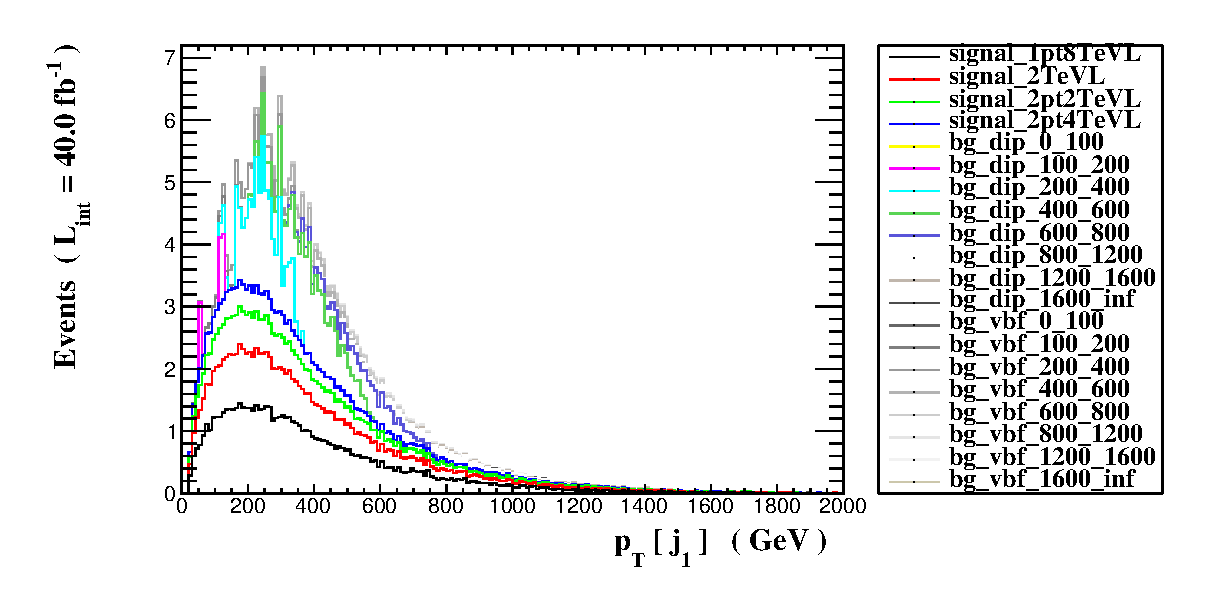
\includegraphics[scale=0.45]{selection_0.eps}\\
\caption{   }
  \end{center}
\end{figure}
      \newpage
\subsection{ Histogram 2}

\textbf{* Plot: ETA ( jets[1] ) }\\
   \begin{table}[H]
  \begin{center}
    \begin{tabular}{|m{23.0mm}|m{23.0mm}|m{18.0mm}|m{19.0mm}|m{19.0mm}|m{19.0mm}|m{19.0mm}|}
      \hline
      {\cellcolor{yellow}         Dataset}& {\cellcolor{yellow}         Integral}& {\cellcolor{yellow}         Entries per event}& {\cellcolor{yellow}         Mean}& {\cellcolor{yellow}         RMS}& {\cellcolor{yellow}         \% underflow}& {\cellcolor{yellow}         \% overflow}\\
      \hline
      {\cellcolor{white}         signal\_1pt8tevl}& {\cellcolor{white}         71.6}& {\cellcolor{white}         1.0}& {\cellcolor{white}         -0.00482515}& {\cellcolor{white}         1.974}& {\cellcolor{green}         0.0}& {\cellcolor{green}         0.0}\\
      \hline
      {\cellcolor{white}         signal\_2tevl}& {\cellcolor{white}         44.7}& {\cellcolor{white}         1.0}& {\cellcolor{white}         -0.00826326}& {\cellcolor{white}         2.002}& {\cellcolor{green}         0.0}& {\cellcolor{green}         0.0}\\
      \hline
      {\cellcolor{white}         signal\_2pt2tevl}& {\cellcolor{white}         29.7}& {\cellcolor{white}         1.0}& {\cellcolor{white}         -0.0199017}& {\cellcolor{white}         2.031}& {\cellcolor{green}         0.0}& {\cellcolor{green}         0.0}\\
      \hline
      {\cellcolor{white}         signal\_2pt4tevl}& {\cellcolor{white}         20.5}& {\cellcolor{white}         1.0}& {\cellcolor{white}         -0.00273609}& {\cellcolor{white}         2.04}& {\cellcolor{green}         0.0}& {\cellcolor{green}         0.0}\\
      \hline
      {\cellcolor{white}         bg\_dip\_0\_100}& {\cellcolor{white}         0.0 +/\-- 0.0}& {\cellcolor{white}         0.}& {\cellcolor{white}         0.0}& {\cellcolor{white}         0.0}& {\cellcolor{green}         0.0}& {\cellcolor{green}         0.0}\\
      \hline
      {\cellcolor{white}         bg\_dip\_100\_200}& {\cellcolor{white}         3.16}& {\cellcolor{white}         1.0}& {\cellcolor{white}         1.65038}& {\cellcolor{white}         2.73}& {\cellcolor{green}         0.0}& {\cellcolor{green}         0.0}\\
      \hline
      {\cellcolor{white}         bg\_dip\_200\_400}& {\cellcolor{white}         25.8}& {\cellcolor{white}         1.0}& {\cellcolor{white}         0.0327822}& {\cellcolor{white}         1.622}& {\cellcolor{green}         0.0}& {\cellcolor{green}         0.0}\\
      \hline
      {\cellcolor{white}         bg\_dip\_400\_600}& {\cellcolor{white}         29.4}& {\cellcolor{white}         1.0}& {\cellcolor{white}         0.0285181}& {\cellcolor{white}         1.387}& {\cellcolor{green}         0.0}& {\cellcolor{green}         0.0}\\
      \hline
      {\cellcolor{white}         bg\_dip\_600\_800}& {\cellcolor{white}         11.9}& {\cellcolor{white}         1.0}& {\cellcolor{white}         -0.0527389}& {\cellcolor{white}         1.256}& {\cellcolor{green}         0.0}& {\cellcolor{green}         0.0}\\
      \hline
      {\cellcolor{white}         bg\_dip\_800\_1200}& {\cellcolor{white}         6.14}& {\cellcolor{white}         1.0}& {\cellcolor{white}         0.00530536}& {\cellcolor{white}         1.183}& {\cellcolor{green}         0.0}& {\cellcolor{green}         0.0}\\
      \hline
      {\cellcolor{white}         bg\_dip\_1200\_1600}& {\cellcolor{white}         0.83}& {\cellcolor{white}         1.0}& {\cellcolor{white}         -0.0573518}& {\cellcolor{white}         1.162}& {\cellcolor{green}         0.0}& {\cellcolor{green}         0.0}\\
      \hline
      {\cellcolor{white}         bg\_dip\_1600\_inf}& {\cellcolor{white}         0.132}& {\cellcolor{white}         1.0}& {\cellcolor{white}         0.0325828}& {\cellcolor{white}         1.171}& {\cellcolor{green}         0.0}& {\cellcolor{green}         0.0}\\
      \hline
      {\cellcolor{white}         bg\_vbf\_0\_100}& {\cellcolor{white}         0.0486}& {\cellcolor{white}         1.0}& {\cellcolor{white}         0.873486}& {\cellcolor{white}         2.934}& {\cellcolor{green}         0.0}& {\cellcolor{green}         0.0}\\
      \hline
      {\cellcolor{white}         bg\_vbf\_100\_200}& {\cellcolor{white}         1.16}& {\cellcolor{white}         1.0}& {\cellcolor{white}         0.133336}& {\cellcolor{white}         2.773}& {\cellcolor{green}         0.0}& {\cellcolor{green}         0.0}\\
      \hline
      {\cellcolor{white}         bg\_vbf\_200\_400}& {\cellcolor{white}         6.68}& {\cellcolor{white}         1.0}& {\cellcolor{white}         0.0158882}& {\cellcolor{white}         2.195}& {\cellcolor{green}         0.0}& {\cellcolor{green}         0.0}\\
      \hline
      {\cellcolor{white}         bg\_vbf\_400\_600}& {\cellcolor{white}         6.68}& {\cellcolor{white}         1.0}& {\cellcolor{white}         -0.0253292}& {\cellcolor{white}         1.796}& {\cellcolor{green}         0.0}& {\cellcolor{green}         0.0}\\
      \hline
      {\cellcolor{white}         bg\_vbf\_600\_800}& {\cellcolor{white}         3.03}& {\cellcolor{white}         1.0}& {\cellcolor{white}         -0.000919668}& {\cellcolor{white}         1.589}& {\cellcolor{green}         0.0}& {\cellcolor{green}         0.0}\\
      \hline
      {\cellcolor{white}         bg\_vbf\_800\_1200}& {\cellcolor{white}         1.58}& {\cellcolor{white}         1.0}& {\cellcolor{white}         -0.0271121}& {\cellcolor{white}         1.423}& {\cellcolor{green}         0.0}& {\cellcolor{green}         0.0}\\
      \hline
      {\cellcolor{white}         bg\_vbf\_1200\_1600}& {\cellcolor{white}         0.236}& {\cellcolor{white}         1.0}& {\cellcolor{white}         -0.0196162}& {\cellcolor{white}         1.285}& {\cellcolor{green}         0.0}& {\cellcolor{green}         0.0}\\
      \hline
      {\cellcolor{white}         bg\_vbf\_1600\_inf}& {\cellcolor{white}         0.0444}& {\cellcolor{white}         1.0}& {\cellcolor{white}         0.0503087}& {\cellcolor{white}         1.194}& {\cellcolor{green}         0.0}& {\cellcolor{green}         0.0}\\
\hline
    \end{tabular}
  \end{center}
\end{table}

\begin{figure}[H]
  \begin{center}
    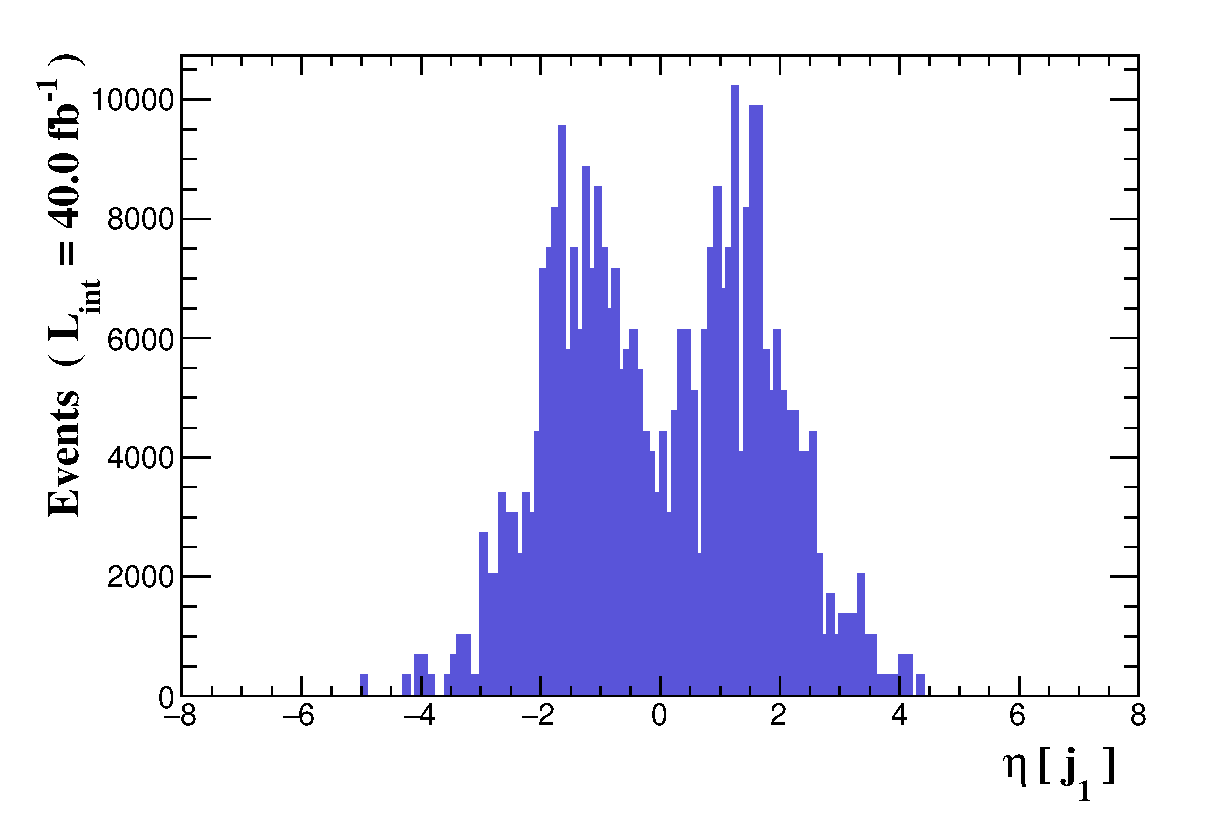
\includegraphics[scale=0.45]{selection_1.eps}\\
\caption{   }
  \end{center}
\end{figure}
      \newpage
\subsection{ Histogram 3}

\textbf{* Plot: PHI ( jets[1] ) }\\
   \begin{table}[H]
  \begin{center}
    \begin{tabular}{|m{23.0mm}|m{23.0mm}|m{18.0mm}|m{19.0mm}|m{19.0mm}|m{19.0mm}|m{19.0mm}|}
      \hline
      {\cellcolor{yellow}         Dataset}& {\cellcolor{yellow}         Integral}& {\cellcolor{yellow}         Entries per event}& {\cellcolor{yellow}         Mean}& {\cellcolor{yellow}         RMS}& {\cellcolor{yellow}         \% underflow}& {\cellcolor{yellow}         \% overflow}\\
      \hline
      {\cellcolor{white}         signal\_1pt8tevl}& {\cellcolor{white}         71.6}& {\cellcolor{white}         1.0}& {\cellcolor{white}         0.00430839}& {\cellcolor{white}         1.812}& {\cellcolor{green}         0.0}& {\cellcolor{green}         0.0}\\
      \hline
      {\cellcolor{white}         signal\_2tevl}& {\cellcolor{white}         44.7}& {\cellcolor{white}         1.0}& {\cellcolor{white}         -0.000657404}& {\cellcolor{white}         1.827}& {\cellcolor{green}         0.0}& {\cellcolor{green}         0.0}\\
      \hline
      {\cellcolor{white}         signal\_2pt2tevl}& {\cellcolor{white}         29.7}& {\cellcolor{white}         1.0}& {\cellcolor{white}         0.0120395}& {\cellcolor{white}         1.816}& {\cellcolor{green}         0.0}& {\cellcolor{green}         0.0}\\
      \hline
      {\cellcolor{white}         signal\_2pt4tevl}& {\cellcolor{white}         20.5}& {\cellcolor{white}         1.0}& {\cellcolor{white}         -0.0272324}& {\cellcolor{white}         1.818}& {\cellcolor{green}         0.0}& {\cellcolor{green}         0.0}\\
      \hline
      {\cellcolor{white}         bg\_dip\_0\_100}& {\cellcolor{white}         0.0 +/\-- 0.0}& {\cellcolor{white}         0.}& {\cellcolor{white}         0.0}& {\cellcolor{white}         0.0}& {\cellcolor{green}         0.0}& {\cellcolor{green}         0.0}\\
      \hline
      {\cellcolor{white}         bg\_dip\_100\_200}& {\cellcolor{white}         3.16}& {\cellcolor{white}         1.0}& {\cellcolor{white}         0.466209}& {\cellcolor{white}         0.3607}& {\cellcolor{green}         0.0}& {\cellcolor{green}         0.0}\\
      \hline
      {\cellcolor{white}         bg\_dip\_200\_400}& {\cellcolor{white}         25.8}& {\cellcolor{white}         1.0}& {\cellcolor{white}         -0.0184691}& {\cellcolor{white}         1.809}& {\cellcolor{green}         0.0}& {\cellcolor{green}         0.0}\\
      \hline
      {\cellcolor{white}         bg\_dip\_400\_600}& {\cellcolor{white}         29.4}& {\cellcolor{white}         1.0}& {\cellcolor{white}         -0.0145545}& {\cellcolor{white}         1.833}& {\cellcolor{green}         0.0}& {\cellcolor{green}         0.0}\\
      \hline
      {\cellcolor{white}         bg\_dip\_600\_800}& {\cellcolor{white}         11.9}& {\cellcolor{white}         1.0}& {\cellcolor{white}         -0.0166173}& {\cellcolor{white}         1.856}& {\cellcolor{green}         0.0}& {\cellcolor{green}         0.0}\\
      \hline
      {\cellcolor{white}         bg\_dip\_800\_1200}& {\cellcolor{white}         6.14}& {\cellcolor{white}         1.0}& {\cellcolor{white}         -6.42725e-05}& {\cellcolor{white}         1.794}& {\cellcolor{green}         0.0}& {\cellcolor{green}         0.0}\\
      \hline
      {\cellcolor{white}         bg\_dip\_1200\_1600}& {\cellcolor{white}         0.83}& {\cellcolor{white}         1.0}& {\cellcolor{white}         -0.00691131}& {\cellcolor{white}         1.856}& {\cellcolor{green}         0.0}& {\cellcolor{green}         0.0}\\
      \hline
      {\cellcolor{white}         bg\_dip\_1600\_inf}& {\cellcolor{white}         0.132}& {\cellcolor{white}         1.0}& {\cellcolor{white}         0.0937289}& {\cellcolor{white}         1.81}& {\cellcolor{green}         0.0}& {\cellcolor{green}         0.0}\\
      \hline
      {\cellcolor{white}         bg\_vbf\_0\_100}& {\cellcolor{white}         0.0486}& {\cellcolor{white}         1.0}& {\cellcolor{white}         -0.168141}& {\cellcolor{white}         1.997}& {\cellcolor{green}         0.0}& {\cellcolor{green}         0.0}\\
      \hline
      {\cellcolor{white}         bg\_vbf\_100\_200}& {\cellcolor{white}         1.16}& {\cellcolor{white}         1.0}& {\cellcolor{white}         -0.0767497}& {\cellcolor{white}         1.778}& {\cellcolor{green}         0.0}& {\cellcolor{green}         0.0}\\
      \hline
      {\cellcolor{white}         bg\_vbf\_200\_400}& {\cellcolor{white}         6.68}& {\cellcolor{white}         1.0}& {\cellcolor{white}         -0.0861787}& {\cellcolor{white}         1.817}& {\cellcolor{green}         0.0}& {\cellcolor{green}         0.0}\\
      \hline
      {\cellcolor{white}         bg\_vbf\_400\_600}& {\cellcolor{white}         6.68}& {\cellcolor{white}         1.0}& {\cellcolor{white}         0.0190635}& {\cellcolor{white}         1.803}& {\cellcolor{green}         0.0}& {\cellcolor{green}         0.0}\\
      \hline
      {\cellcolor{white}         bg\_vbf\_600\_800}& {\cellcolor{white}         3.03}& {\cellcolor{white}         1.0}& {\cellcolor{white}         -0.00814006}& {\cellcolor{white}         1.804}& {\cellcolor{green}         0.0}& {\cellcolor{green}         0.0}\\
      \hline
      {\cellcolor{white}         bg\_vbf\_800\_1200}& {\cellcolor{white}         1.58}& {\cellcolor{white}         1.0}& {\cellcolor{white}         0.0406637}& {\cellcolor{white}         1.81}& {\cellcolor{green}         0.0}& {\cellcolor{green}         0.0}\\
      \hline
      {\cellcolor{white}         bg\_vbf\_1200\_1600}& {\cellcolor{white}         0.236}& {\cellcolor{white}         1.0}& {\cellcolor{white}         0.0203858}& {\cellcolor{white}         1.807}& {\cellcolor{green}         0.0}& {\cellcolor{green}         0.0}\\
      \hline
      {\cellcolor{white}         bg\_vbf\_1600\_inf}& {\cellcolor{white}         0.0444}& {\cellcolor{white}         1.0}& {\cellcolor{white}         0.0571332}& {\cellcolor{white}         1.824}& {\cellcolor{green}         0.0}& {\cellcolor{green}         0.0}\\
\hline
    \end{tabular}
  \end{center}
\end{table}

\begin{figure}[H]
  \begin{center}
    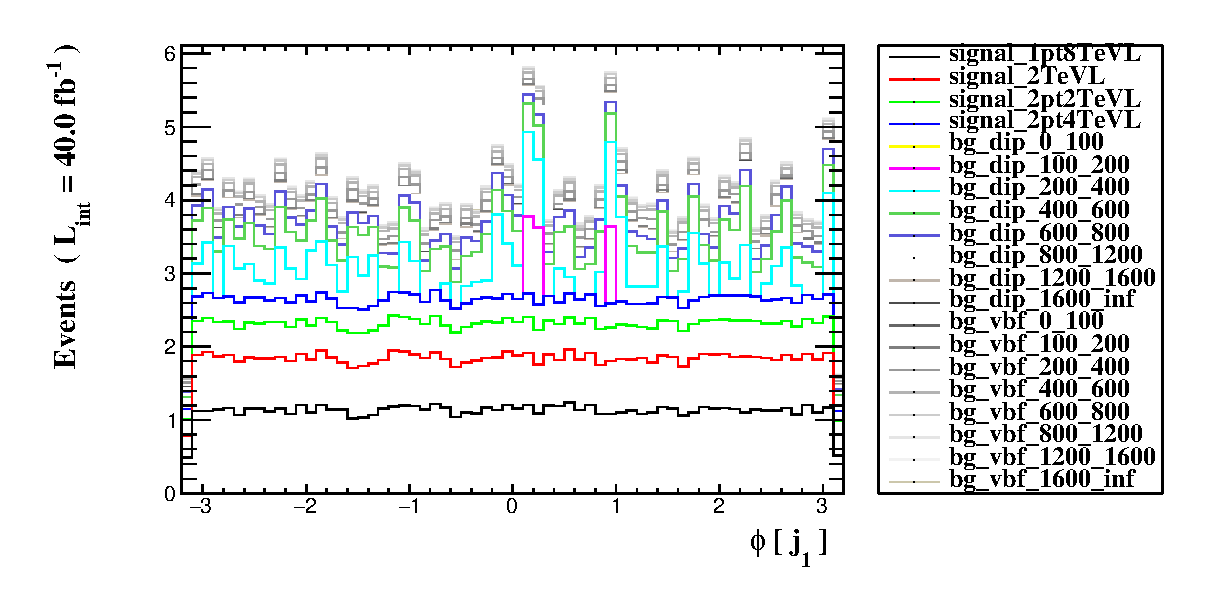
\includegraphics[scale=0.45]{selection_2.eps}\\
\caption{   }
  \end{center}
\end{figure}
      \newpage
\subsection{ Histogram 4}

\textbf{* Plot: PT ( jets[2] ) }\\
   \begin{table}[H]
  \begin{center}
    \begin{tabular}{|m{23.0mm}|m{23.0mm}|m{18.0mm}|m{19.0mm}|m{19.0mm}|m{19.0mm}|m{19.0mm}|}
      \hline
      {\cellcolor{yellow}         Dataset}& {\cellcolor{yellow}         Integral}& {\cellcolor{yellow}         Entries per event}& {\cellcolor{yellow}         Mean}& {\cellcolor{yellow}         RMS}& {\cellcolor{yellow}         \% underflow}& {\cellcolor{yellow}         \% overflow}\\
      \hline
      {\cellcolor{white}         signal\_1pt8tevl}& {\cellcolor{white}         71.6}& {\cellcolor{white}         1.0}& {\cellcolor{white}         126.672}& {\cellcolor{white}         102.5}& {\cellcolor{green}         0.0}& {\cellcolor{green}         0.004942}\\
      \hline
      {\cellcolor{white}         signal\_2tevl}& {\cellcolor{white}         44.7}& {\cellcolor{white}         1.0}& {\cellcolor{white}         122.114}& {\cellcolor{white}         98.76}& {\cellcolor{green}         0.0}& {\cellcolor{green}         0.004778}\\
      \hline
      {\cellcolor{white}         signal\_2pt2tevl}& {\cellcolor{white}         29.7}& {\cellcolor{white}         1.0}& {\cellcolor{white}         119.452}& {\cellcolor{white}         96.18}& {\cellcolor{green}         0.0}& {\cellcolor{green}         0.002341}\\
      \hline
      {\cellcolor{white}         signal\_2pt4tevl}& {\cellcolor{white}         20.5}& {\cellcolor{white}         1.0}& {\cellcolor{white}         117.516}& {\cellcolor{white}         94.67}& {\cellcolor{green}         0.0}& {\cellcolor{green}         0.006934}\\
      \hline
      {\cellcolor{white}         bg\_dip\_0\_100}& {\cellcolor{white}         0.0 +/\-- 0.0}& {\cellcolor{white}         0.}& {\cellcolor{white}         0.0}& {\cellcolor{white}         0.0}& {\cellcolor{green}         0.0}& {\cellcolor{green}         0.0}\\
      \hline
      {\cellcolor{white}         bg\_dip\_100\_200}& {\cellcolor{white}         3.16}& {\cellcolor{white}         1.0}& {\cellcolor{white}         49.3379}& {\cellcolor{white}         16.83}& {\cellcolor{green}         0.0}& {\cellcolor{green}         0.0}\\
      \hline
      {\cellcolor{white}         bg\_dip\_200\_400}& {\cellcolor{white}         25.8}& {\cellcolor{white}         1.0}& {\cellcolor{white}         80.1038}& {\cellcolor{white}         38.82}& {\cellcolor{green}         0.0}& {\cellcolor{green}         0.0}\\
      \hline
      {\cellcolor{white}         bg\_dip\_400\_600}& {\cellcolor{white}         29.4}& {\cellcolor{white}         1.0}& {\cellcolor{white}         109.934}& {\cellcolor{white}         61.83}& {\cellcolor{green}         0.0}& {\cellcolor{green}         0.0}\\
      \hline
      {\cellcolor{white}         bg\_dip\_600\_800}& {\cellcolor{white}         11.9}& {\cellcolor{white}         1.0}& {\cellcolor{white}         141.464}& {\cellcolor{white}         92.51}& {\cellcolor{green}         0.0}& {\cellcolor{green}         0.0}\\
      \hline
      {\cellcolor{white}         bg\_dip\_800\_1200}& {\cellcolor{white}         6.14}& {\cellcolor{white}         1.0}& {\cellcolor{white}         192.947}& {\cellcolor{white}         137.0}& {\cellcolor{green}         0.0}& {\cellcolor{green}         0.0}\\
      \hline
      {\cellcolor{white}         bg\_dip\_1200\_1600}& {\cellcolor{white}         0.83}& {\cellcolor{white}         1.0}& {\cellcolor{white}         316.424}& {\cellcolor{white}         222.2}& {\cellcolor{green}         0.0}& {\cellcolor{green}         0.0}\\
      \hline
      {\cellcolor{white}         bg\_dip\_1600\_inf}& {\cellcolor{white}         0.132}& {\cellcolor{white}         1.0}& {\cellcolor{white}         538.488}& {\cellcolor{white}         322.1}& {\cellcolor{green}         0.0}& {\cellcolor{green}         4.526}\\
      \hline
      {\cellcolor{white}         bg\_vbf\_0\_100}& {\cellcolor{white}         0.0486}& {\cellcolor{white}         1.0}& {\cellcolor{white}         31.916}& {\cellcolor{white}         8.29}& {\cellcolor{green}         0.0}& {\cellcolor{green}         0.0}\\
      \hline
      {\cellcolor{white}         bg\_vbf\_100\_200}& {\cellcolor{white}         1.16}& {\cellcolor{white}         1.0}& {\cellcolor{white}         53.936}& {\cellcolor{white}         17.53}& {\cellcolor{green}         0.0}& {\cellcolor{green}         0.0}\\
      \hline
      {\cellcolor{white}         bg\_vbf\_200\_400}& {\cellcolor{white}         6.68}& {\cellcolor{white}         1.0}& {\cellcolor{white}         94.1307}& {\cellcolor{white}         38.71}& {\cellcolor{green}         0.0}& {\cellcolor{green}         0.0}\\
      \hline
      {\cellcolor{white}         bg\_vbf\_400\_600}& {\cellcolor{white}         6.68}& {\cellcolor{white}         1.0}& {\cellcolor{white}         133.026}& {\cellcolor{white}         59.99}& {\cellcolor{green}         0.0}& {\cellcolor{green}         0.0}\\
      \hline
      {\cellcolor{white}         bg\_vbf\_600\_800}& {\cellcolor{white}         3.03}& {\cellcolor{white}         1.0}& {\cellcolor{white}         180.549}& {\cellcolor{white}         86.09}& {\cellcolor{green}         0.0}& {\cellcolor{green}         0.0}\\
      \hline
      {\cellcolor{white}         bg\_vbf\_800\_1200}& {\cellcolor{white}         1.58}& {\cellcolor{white}         1.0}& {\cellcolor{white}         244.294}& {\cellcolor{white}         127.1}& {\cellcolor{green}         0.0}& {\cellcolor{green}         0.0}\\
      \hline
      {\cellcolor{white}         bg\_vbf\_1200\_1600}& {\cellcolor{white}         0.236}& {\cellcolor{white}         1.0}& {\cellcolor{white}         367.183}& {\cellcolor{white}         193.0}& {\cellcolor{green}         0.0}& {\cellcolor{green}         0.0}\\
      \hline
      {\cellcolor{white}         bg\_vbf\_1600\_inf}& {\cellcolor{white}         0.0444}& {\cellcolor{white}         1.0}& {\cellcolor{white}         520.042}& {\cellcolor{white}         285.6}& {\cellcolor{green}         0.0}& {\cellcolor{green}         2.43}\\
\hline
    \end{tabular}
  \end{center}
\end{table}

\begin{figure}[H]
  \begin{center}
    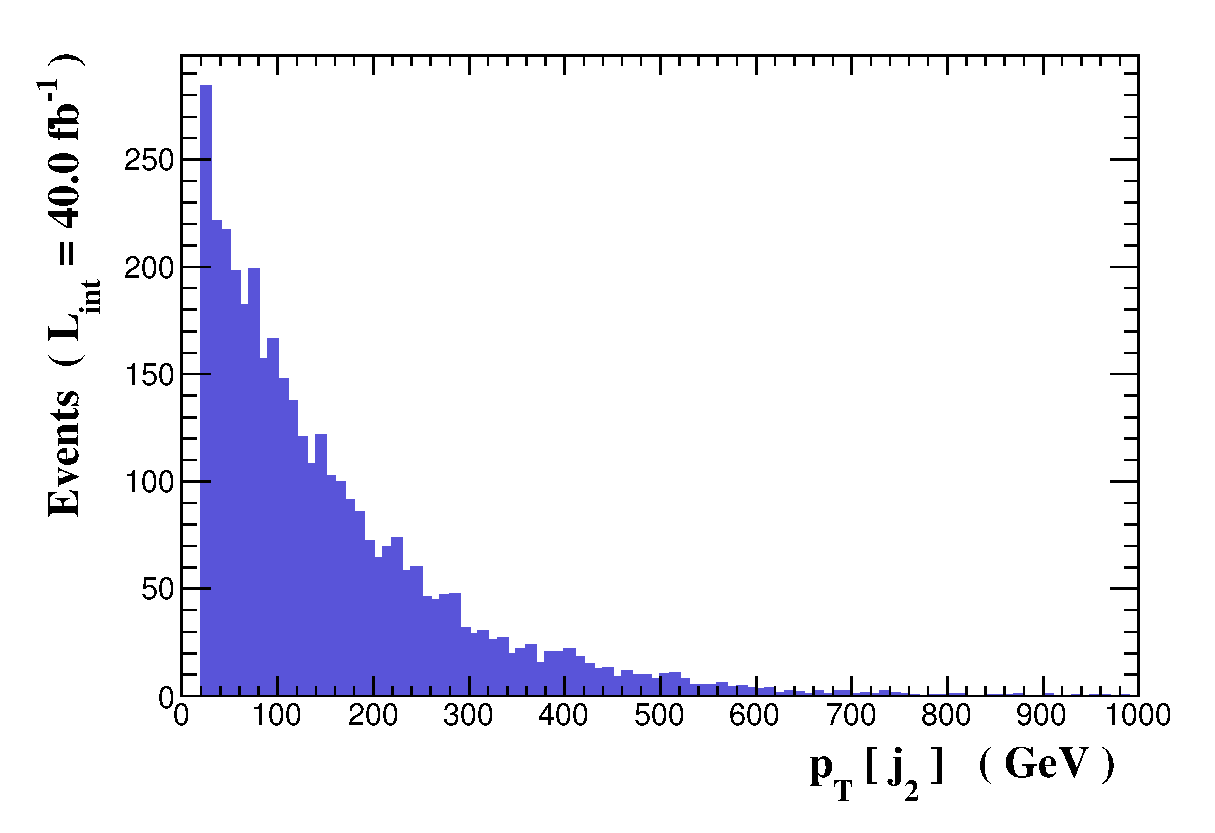
\includegraphics[scale=0.45]{selection_3.eps}\\
\caption{   }
  \end{center}
\end{figure}
      \newpage
\subsection{ Histogram 5}

\textbf{* Plot: ETA ( jets[2] ) }\\
   \begin{table}[H]
  \begin{center}
    \begin{tabular}{|m{23.0mm}|m{23.0mm}|m{18.0mm}|m{19.0mm}|m{19.0mm}|m{19.0mm}|m{19.0mm}|}
      \hline
      {\cellcolor{yellow}         Dataset}& {\cellcolor{yellow}         Integral}& {\cellcolor{yellow}         Entries per event}& {\cellcolor{yellow}         Mean}& {\cellcolor{yellow}         RMS}& {\cellcolor{yellow}         \% underflow}& {\cellcolor{yellow}         \% overflow}\\
      \hline
      {\cellcolor{white}         signal\_1pt8tevl}& {\cellcolor{white}         71.6}& {\cellcolor{white}         1.0}& {\cellcolor{white}         -0.00273279}& {\cellcolor{white}         2.847}& {\cellcolor{green}         0.0}& {\cellcolor{green}         0.0}\\
      \hline
      {\cellcolor{white}         signal\_2tevl}& {\cellcolor{white}         44.7}& {\cellcolor{white}         1.0}& {\cellcolor{white}         -0.00636076}& {\cellcolor{white}         2.886}& {\cellcolor{green}         0.0}& {\cellcolor{green}         0.0}\\
      \hline
      {\cellcolor{white}         signal\_2pt2tevl}& {\cellcolor{white}         29.7}& {\cellcolor{white}         1.0}& {\cellcolor{white}         0.0204261}& {\cellcolor{white}         2.905}& {\cellcolor{green}         0.0}& {\cellcolor{green}         0.0}\\
      \hline
      {\cellcolor{white}         signal\_2pt4tevl}& {\cellcolor{white}         20.5}& {\cellcolor{white}         1.0}& {\cellcolor{white}         0.00378007}& {\cellcolor{white}         2.919}& {\cellcolor{green}         0.0}& {\cellcolor{green}         0.0}\\
      \hline
      {\cellcolor{white}         bg\_dip\_0\_100}& {\cellcolor{white}         0.0 +/\-- 0.0}& {\cellcolor{white}         0.}& {\cellcolor{white}         0.0}& {\cellcolor{white}         0.0}& {\cellcolor{green}         0.0}& {\cellcolor{green}         0.0}\\
      \hline
      {\cellcolor{white}         bg\_dip\_100\_200}& {\cellcolor{white}         3.16}& {\cellcolor{white}         1.0}& {\cellcolor{white}         0.140052}& {\cellcolor{white}         2.918}& {\cellcolor{green}         0.0}& {\cellcolor{green}         0.0}\\
      \hline
      {\cellcolor{white}         bg\_dip\_200\_400}& {\cellcolor{white}         25.8}& {\cellcolor{white}         1.0}& {\cellcolor{white}         0.341283}& {\cellcolor{white}         2.913}& {\cellcolor{green}         0.0}& {\cellcolor{green}         0.0}\\
      \hline
      {\cellcolor{white}         bg\_dip\_400\_600}& {\cellcolor{white}         29.4}& {\cellcolor{white}         1.0}& {\cellcolor{white}         0.0011524}& {\cellcolor{white}         2.601}& {\cellcolor{green}         0.0}& {\cellcolor{green}         0.0}\\
      \hline
      {\cellcolor{white}         bg\_dip\_600\_800}& {\cellcolor{white}         11.9}& {\cellcolor{white}         1.0}& {\cellcolor{white}         0.0476112}& {\cellcolor{white}         2.556}& {\cellcolor{green}         0.0}& {\cellcolor{green}         0.0}\\
      \hline
      {\cellcolor{white}         bg\_dip\_800\_1200}& {\cellcolor{white}         6.14}& {\cellcolor{white}         1.0}& {\cellcolor{white}         -0.0409596}& {\cellcolor{white}         2.481}& {\cellcolor{green}         0.0}& {\cellcolor{green}         0.0}\\
      \hline
      {\cellcolor{white}         bg\_dip\_1200\_1600}& {\cellcolor{white}         0.83}& {\cellcolor{white}         1.0}& {\cellcolor{white}         0.043888}& {\cellcolor{white}         2.297}& {\cellcolor{green}         0.0}& {\cellcolor{green}         0.0}\\
      \hline
      {\cellcolor{white}         bg\_dip\_1600\_inf}& {\cellcolor{white}         0.132}& {\cellcolor{white}         1.0}& {\cellcolor{white}         -0.122585}& {\cellcolor{white}         2.088}& {\cellcolor{green}         0.0}& {\cellcolor{green}         0.0}\\
      \hline
      {\cellcolor{white}         bg\_vbf\_0\_100}& {\cellcolor{white}         0.0486}& {\cellcolor{white}         1.0}& {\cellcolor{white}         1.04772}& {\cellcolor{white}         3.507}& {\cellcolor{green}         0.0}& {\cellcolor{green}         0.0}\\
      \hline
      {\cellcolor{white}         bg\_vbf\_100\_200}& {\cellcolor{white}         1.16}& {\cellcolor{white}         1.0}& {\cellcolor{white}         -0.324417}& {\cellcolor{white}         3.174}& {\cellcolor{green}         0.0}& {\cellcolor{green}         0.0}\\
      \hline
      {\cellcolor{white}         bg\_vbf\_200\_400}& {\cellcolor{white}         6.68}& {\cellcolor{white}         1.0}& {\cellcolor{white}         0.0369757}& {\cellcolor{white}         2.866}& {\cellcolor{green}         0.0}& {\cellcolor{green}         0.0}\\
      \hline
      {\cellcolor{white}         bg\_vbf\_400\_600}& {\cellcolor{white}         6.68}& {\cellcolor{white}         1.0}& {\cellcolor{white}         0.0499887}& {\cellcolor{white}         2.594}& {\cellcolor{green}         0.0}& {\cellcolor{green}         0.0}\\
      \hline
      {\cellcolor{white}         bg\_vbf\_600\_800}& {\cellcolor{white}         3.03}& {\cellcolor{white}         1.0}& {\cellcolor{white}         0.00439739}& {\cellcolor{white}         2.453}& {\cellcolor{green}         0.0}& {\cellcolor{green}         0.0}\\
      \hline
      {\cellcolor{white}         bg\_vbf\_800\_1200}& {\cellcolor{white}         1.58}& {\cellcolor{white}         1.0}& {\cellcolor{white}         0.0359424}& {\cellcolor{white}         2.343}& {\cellcolor{green}         0.0}& {\cellcolor{green}         0.0}\\
      \hline
      {\cellcolor{white}         bg\_vbf\_1200\_1600}& {\cellcolor{white}         0.236}& {\cellcolor{white}         1.0}& {\cellcolor{white}         0.0450563}& {\cellcolor{white}         2.208}& {\cellcolor{green}         0.0}& {\cellcolor{green}         0.0}\\
      \hline
      {\cellcolor{white}         bg\_vbf\_1600\_inf}& {\cellcolor{white}         0.0444}& {\cellcolor{white}         1.0}& {\cellcolor{white}         -0.0663344}& {\cellcolor{white}         2.114}& {\cellcolor{green}         0.0}& {\cellcolor{green}         0.0}\\
\hline
    \end{tabular}
  \end{center}
\end{table}

\begin{figure}[H]
  \begin{center}
    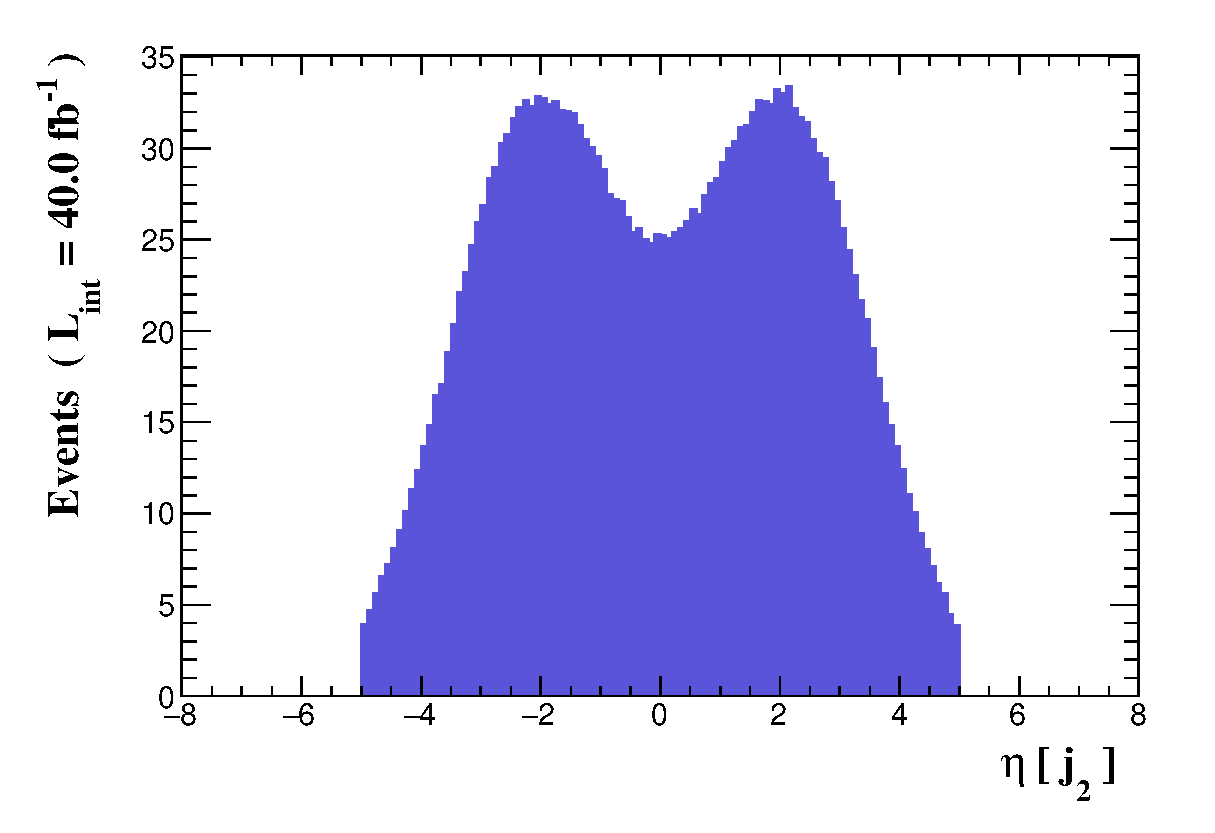
\includegraphics[scale=0.45]{selection_4.eps}\\
\caption{   }
  \end{center}
\end{figure}
      \newpage
\subsection{ Histogram 6}

\textbf{* Plot: PHI ( jets[2] ) }\\
   \begin{table}[H]
  \begin{center}
    \begin{tabular}{|m{23.0mm}|m{23.0mm}|m{18.0mm}|m{19.0mm}|m{19.0mm}|m{19.0mm}|m{19.0mm}|}
      \hline
      {\cellcolor{yellow}         Dataset}& {\cellcolor{yellow}         Integral}& {\cellcolor{yellow}         Entries per event}& {\cellcolor{yellow}         Mean}& {\cellcolor{yellow}         RMS}& {\cellcolor{yellow}         \% underflow}& {\cellcolor{yellow}         \% overflow}\\
      \hline
      {\cellcolor{white}         signal\_1pt8tevl}& {\cellcolor{white}         71.6}& {\cellcolor{white}         1.0}& {\cellcolor{white}         -0.00551197}& {\cellcolor{white}         1.813}& {\cellcolor{green}         0.0}& {\cellcolor{green}         0.0}\\
      \hline
      {\cellcolor{white}         signal\_2tevl}& {\cellcolor{white}         44.7}& {\cellcolor{white}         1.0}& {\cellcolor{white}         -0.00629482}& {\cellcolor{white}         1.815}& {\cellcolor{green}         0.0}& {\cellcolor{green}         0.0}\\
      \hline
      {\cellcolor{white}         signal\_2pt2tevl}& {\cellcolor{white}         29.7}& {\cellcolor{white}         1.0}& {\cellcolor{white}         0.00123806}& {\cellcolor{white}         1.811}& {\cellcolor{green}         0.0}& {\cellcolor{green}         0.0}\\
      \hline
      {\cellcolor{white}         signal\_2pt4tevl}& {\cellcolor{white}         20.5}& {\cellcolor{white}         1.0}& {\cellcolor{white}         -0.00251439}& {\cellcolor{white}         1.808}& {\cellcolor{green}         0.0}& {\cellcolor{green}         0.0}\\
      \hline
      {\cellcolor{white}         bg\_dip\_0\_100}& {\cellcolor{white}         0.0 +/\-- 0.0}& {\cellcolor{white}         0.}& {\cellcolor{white}         0.0}& {\cellcolor{white}         0.0}& {\cellcolor{green}         0.0}& {\cellcolor{green}         0.0}\\
      \hline
      {\cellcolor{white}         bg\_dip\_100\_200}& {\cellcolor{white}         3.16}& {\cellcolor{white}         1.0}& {\cellcolor{white}         1.00733}& {\cellcolor{white}         1.634}& {\cellcolor{green}         0.0}& {\cellcolor{green}         0.0}\\
      \hline
      {\cellcolor{white}         bg\_dip\_200\_400}& {\cellcolor{white}         25.8}& {\cellcolor{white}         1.0}& {\cellcolor{white}         -0.0150701}& {\cellcolor{white}         1.924}& {\cellcolor{green}         0.0}& {\cellcolor{green}         0.0}\\
      \hline
      {\cellcolor{white}         bg\_dip\_400\_600}& {\cellcolor{white}         29.4}& {\cellcolor{white}         1.0}& {\cellcolor{white}         -0.020964}& {\cellcolor{white}         1.794}& {\cellcolor{green}         0.0}& {\cellcolor{green}         0.0}\\
      \hline
      {\cellcolor{white}         bg\_dip\_600\_800}& {\cellcolor{white}         11.9}& {\cellcolor{white}         1.0}& {\cellcolor{white}         0.0543267}& {\cellcolor{white}         1.792}& {\cellcolor{green}         0.0}& {\cellcolor{green}         0.0}\\
      \hline
      {\cellcolor{white}         bg\_dip\_800\_1200}& {\cellcolor{white}         6.14}& {\cellcolor{white}         1.0}& {\cellcolor{white}         0.0379614}& {\cellcolor{white}         1.804}& {\cellcolor{green}         0.0}& {\cellcolor{green}         0.0}\\
      \hline
      {\cellcolor{white}         bg\_dip\_1200\_1600}& {\cellcolor{white}         0.83}& {\cellcolor{white}         1.0}& {\cellcolor{white}         -0.0236384}& {\cellcolor{white}         1.819}& {\cellcolor{green}         0.0}& {\cellcolor{green}         0.0}\\
      \hline
      {\cellcolor{white}         bg\_dip\_1600\_inf}& {\cellcolor{white}         0.132}& {\cellcolor{white}         1.0}& {\cellcolor{white}         -0.168036}& {\cellcolor{white}         1.827}& {\cellcolor{green}         0.0}& {\cellcolor{green}         0.0}\\
      \hline
      {\cellcolor{white}         bg\_vbf\_0\_100}& {\cellcolor{white}         0.0486}& {\cellcolor{white}         1.0}& {\cellcolor{white}         0.0859607}& {\cellcolor{white}         1.498}& {\cellcolor{green}         0.0}& {\cellcolor{green}         0.0}\\
      \hline
      {\cellcolor{white}         bg\_vbf\_100\_200}& {\cellcolor{white}         1.16}& {\cellcolor{white}         1.0}& {\cellcolor{white}         0.17327}& {\cellcolor{white}         1.879}& {\cellcolor{green}         0.0}& {\cellcolor{green}         0.0}\\
      \hline
      {\cellcolor{white}         bg\_vbf\_200\_400}& {\cellcolor{white}         6.68}& {\cellcolor{white}         1.0}& {\cellcolor{white}         -0.0623337}& {\cellcolor{white}         1.832}& {\cellcolor{green}         0.0}& {\cellcolor{green}         0.0}\\
      \hline
      {\cellcolor{white}         bg\_vbf\_400\_600}& {\cellcolor{white}         6.68}& {\cellcolor{white}         1.0}& {\cellcolor{white}         -0.0452271}& {\cellcolor{white}         1.825}& {\cellcolor{green}         0.0}& {\cellcolor{green}         0.0}\\
      \hline
      {\cellcolor{white}         bg\_vbf\_600\_800}& {\cellcolor{white}         3.03}& {\cellcolor{white}         1.0}& {\cellcolor{white}         -0.00796522}& {\cellcolor{white}         1.816}& {\cellcolor{green}         0.0}& {\cellcolor{green}         0.0}\\
      \hline
      {\cellcolor{white}         bg\_vbf\_800\_1200}& {\cellcolor{white}         1.58}& {\cellcolor{white}         1.0}& {\cellcolor{white}         -0.0301573}& {\cellcolor{white}         1.811}& {\cellcolor{green}         0.0}& {\cellcolor{green}         0.0}\\
      \hline
      {\cellcolor{white}         bg\_vbf\_1200\_1600}& {\cellcolor{white}         0.236}& {\cellcolor{white}         1.0}& {\cellcolor{white}         -0.0222433}& {\cellcolor{white}         1.824}& {\cellcolor{green}         0.0}& {\cellcolor{green}         0.0}\\
      \hline
      {\cellcolor{white}         bg\_vbf\_1600\_inf}& {\cellcolor{white}         0.0444}& {\cellcolor{white}         1.0}& {\cellcolor{white}         0.0549082}& {\cellcolor{white}         1.783}& {\cellcolor{green}         0.0}& {\cellcolor{green}         0.0}\\
\hline
    \end{tabular}
  \end{center}
\end{table}

\begin{figure}[H]
  \begin{center}
    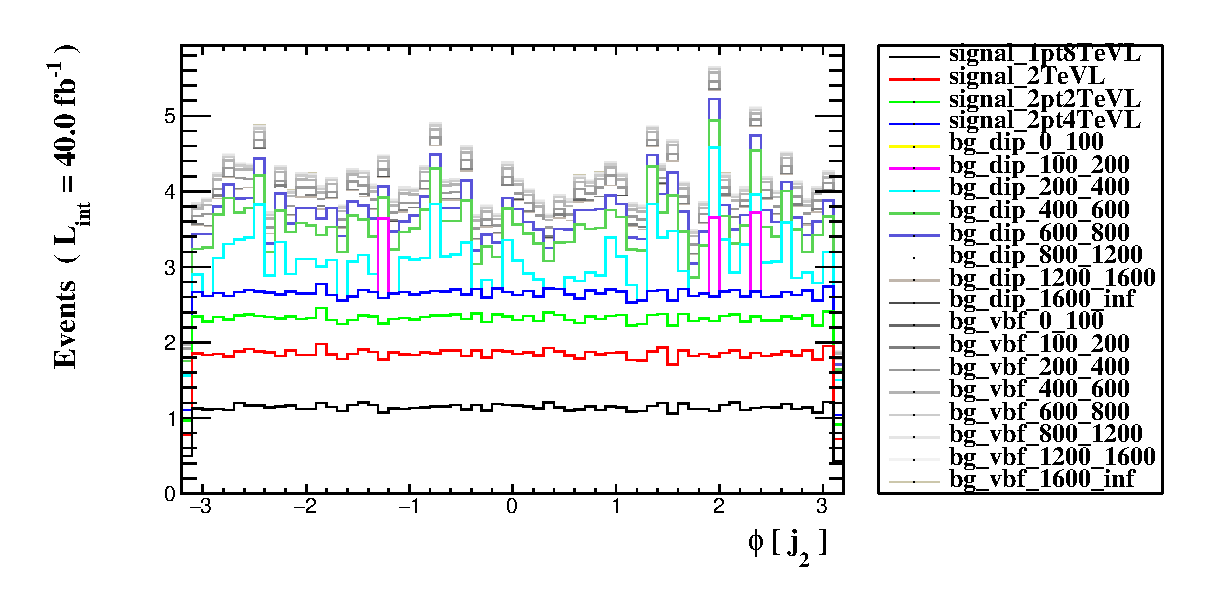
\includegraphics[scale=0.45]{selection_5.eps}\\
\caption{   }
  \end{center}
\end{figure}
      \newpage
\subsection{ Histogram 7}

\textbf{* Plot: DELTAR ( jets[1] , jets[2] ) }\\
   \begin{table}[H]
  \begin{center}
    \begin{tabular}{|m{23.0mm}|m{23.0mm}|m{18.0mm}|m{19.0mm}|m{19.0mm}|m{19.0mm}|m{19.0mm}|}
      \hline
      {\cellcolor{yellow}         Dataset}& {\cellcolor{yellow}         Integral}& {\cellcolor{yellow}         Entries per event}& {\cellcolor{yellow}         Mean}& {\cellcolor{yellow}         RMS}& {\cellcolor{yellow}         \% underflow}& {\cellcolor{yellow}         \% overflow}\\
      \hline
      {\cellcolor{white}         signal\_1pt8tevl}& {\cellcolor{white}         71.6}& {\cellcolor{white}         1.0}& {\cellcolor{white}         4.7913}& {\cellcolor{white}         1.264}& {\cellcolor{green}         0.0}& {\cellcolor{green}         0.0}\\
      \hline
      {\cellcolor{white}         signal\_2tevl}& {\cellcolor{white}         44.7}& {\cellcolor{white}         1.0}& {\cellcolor{white}         4.85016}& {\cellcolor{white}         1.269}& {\cellcolor{green}         0.0}& {\cellcolor{green}         0.0}\\
      \hline
      {\cellcolor{white}         signal\_2pt2tevl}& {\cellcolor{white}         29.7}& {\cellcolor{white}         1.0}& {\cellcolor{white}         4.89784}& {\cellcolor{white}         1.272}& {\cellcolor{green}         0.0}& {\cellcolor{green}         0.0}\\
      \hline
      {\cellcolor{white}         signal\_2pt4tevl}& {\cellcolor{white}         20.5}& {\cellcolor{white}         1.0}& {\cellcolor{white}         4.91461}& {\cellcolor{white}         1.273}& {\cellcolor{green}         0.0}& {\cellcolor{green}         0.0}\\
      \hline
      {\cellcolor{white}         bg\_dip\_0\_100}& {\cellcolor{white}         0.0 +/\-- 0.0}& {\cellcolor{white}         0.}& {\cellcolor{white}         0.0}& {\cellcolor{white}         0.0}& {\cellcolor{green}         0.0}& {\cellcolor{green}         0.0}\\
      \hline
      {\cellcolor{white}         bg\_dip\_100\_200}& {\cellcolor{white}         3.16}& {\cellcolor{white}         1.0}& {\cellcolor{white}         5.99929}& {\cellcolor{white}         0.4811}& {\cellcolor{green}         0.0}& {\cellcolor{green}         0.0}\\
      \hline
      {\cellcolor{white}         bg\_dip\_200\_400}& {\cellcolor{white}         25.8}& {\cellcolor{white}         1.0}& {\cellcolor{white}         4.61504}& {\cellcolor{white}         0.7198}& {\cellcolor{green}         0.0}& {\cellcolor{green}         0.0}\\
      \hline
      {\cellcolor{white}         bg\_dip\_400\_600}& {\cellcolor{white}         29.4}& {\cellcolor{white}         1.0}& {\cellcolor{white}         4.09991}& {\cellcolor{white}         0.7051}& {\cellcolor{green}         0.0}& {\cellcolor{green}         0.0}\\
      \hline
      {\cellcolor{white}         bg\_dip\_600\_800}& {\cellcolor{white}         11.9}& {\cellcolor{white}         1.0}& {\cellcolor{white}         4.02528}& {\cellcolor{white}         0.6393}& {\cellcolor{green}         0.0}& {\cellcolor{green}         0.0}\\
      \hline
      {\cellcolor{white}         bg\_dip\_800\_1200}& {\cellcolor{white}         6.14}& {\cellcolor{white}         1.0}& {\cellcolor{white}         4.00152}& {\cellcolor{white}         0.5757}& {\cellcolor{green}         0.0}& {\cellcolor{green}         0.0}\\
      \hline
      {\cellcolor{white}         bg\_dip\_1200\_1600}& {\cellcolor{white}         0.83}& {\cellcolor{white}         1.0}& {\cellcolor{white}         3.9588}& {\cellcolor{white}         0.4793}& {\cellcolor{green}         0.0}& {\cellcolor{green}         0.0}\\
      \hline
      {\cellcolor{white}         bg\_dip\_1600\_inf}& {\cellcolor{white}         0.132}& {\cellcolor{white}         1.0}& {\cellcolor{white}         3.95712}& {\cellcolor{white}         0.4082}& {\cellcolor{green}         0.0}& {\cellcolor{green}         0.0}\\
      \hline
      {\cellcolor{white}         bg\_vbf\_0\_100}& {\cellcolor{white}         0.0486}& {\cellcolor{white}         1.0}& {\cellcolor{white}         6.62263}& {\cellcolor{white}         0.3293}& {\cellcolor{green}         0.0}& {\cellcolor{green}         0.0}\\
      \hline
      {\cellcolor{white}         bg\_vbf\_100\_200}& {\cellcolor{white}         1.16}& {\cellcolor{white}         1.0}& {\cellcolor{white}         5.99091}& {\cellcolor{white}         0.8146}& {\cellcolor{green}         0.0}& {\cellcolor{green}         0.0}\\
      \hline
      {\cellcolor{white}         bg\_vbf\_200\_400}& {\cellcolor{white}         6.68}& {\cellcolor{white}         1.0}& {\cellcolor{white}         5.10685}& {\cellcolor{white}         0.9126}& {\cellcolor{green}         0.0}& {\cellcolor{green}         0.0}\\
      \hline
      {\cellcolor{white}         bg\_vbf\_400\_600}& {\cellcolor{white}         6.68}& {\cellcolor{white}         1.0}& {\cellcolor{white}         4.54901}& {\cellcolor{white}         0.8616}& {\cellcolor{green}         0.0}& {\cellcolor{green}         0.0}\\
      \hline
      {\cellcolor{white}         bg\_vbf\_600\_800}& {\cellcolor{white}         3.03}& {\cellcolor{white}         1.0}& {\cellcolor{white}         4.35037}& {\cellcolor{white}         0.747}& {\cellcolor{green}         0.0}& {\cellcolor{green}         0.0}\\
      \hline
      {\cellcolor{white}         bg\_vbf\_800\_1200}& {\cellcolor{white}         1.58}& {\cellcolor{white}         1.0}& {\cellcolor{white}         4.19332}& {\cellcolor{white}         0.6452}& {\cellcolor{green}         0.0}& {\cellcolor{green}         0.0}\\
      \hline
      {\cellcolor{white}         bg\_vbf\_1200\_1600}& {\cellcolor{white}         0.236}& {\cellcolor{white}         1.0}& {\cellcolor{white}         4.06782}& {\cellcolor{white}         0.544}& {\cellcolor{green}         0.0}& {\cellcolor{green}         0.0}\\
      \hline
      {\cellcolor{white}         bg\_vbf\_1600\_inf}& {\cellcolor{white}         0.0444}& {\cellcolor{white}         1.0}& {\cellcolor{white}         4.00588}& {\cellcolor{white}         0.4638}& {\cellcolor{green}         0.0}& {\cellcolor{green}         0.0}\\
\hline
    \end{tabular}
  \end{center}
\end{table}

\begin{figure}[H]
  \begin{center}
    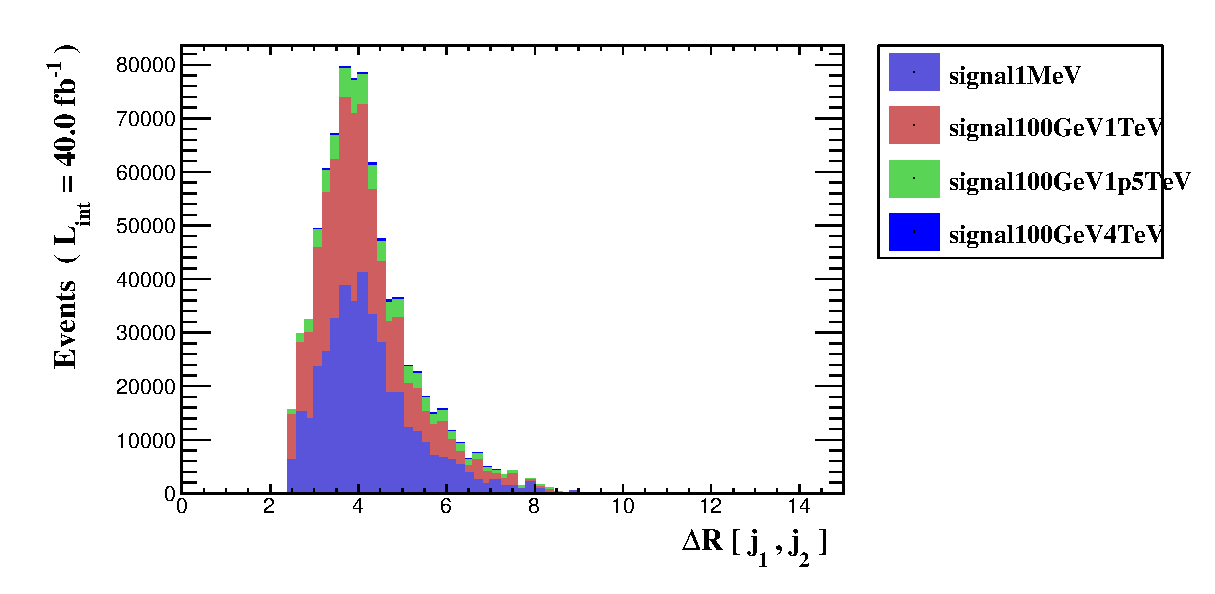
\includegraphics[scale=0.45]{selection_6.eps}\\
\caption{   }
  \end{center}
\end{figure}
      \newpage
\subsection{ Histogram 8}

\textbf{* Plot: M ( jets[1] jets[2] ) }\\
   \begin{table}[H]
  \begin{center}
    \begin{tabular}{|m{23.0mm}|m{23.0mm}|m{18.0mm}|m{19.0mm}|m{19.0mm}|m{19.0mm}|m{19.0mm}|}
      \hline
      {\cellcolor{yellow}         Dataset}& {\cellcolor{yellow}         Integral}& {\cellcolor{yellow}         Entries per event}& {\cellcolor{yellow}         Mean}& {\cellcolor{yellow}         RMS}& {\cellcolor{yellow}         \% underflow}& {\cellcolor{yellow}         \% overflow}\\
      \hline
      {\cellcolor{white}         signal\_1pt8tevl}& {\cellcolor{white}         71.6}& {\cellcolor{white}         1.0}& {\cellcolor{white}         1700.42}& {\cellcolor{white}         795.4}& {\cellcolor{green}         0.0}& {\cellcolor{green}         0.0}\\
      \hline
      {\cellcolor{white}         signal\_2tevl}& {\cellcolor{white}         44.7}& {\cellcolor{white}         1.0}& {\cellcolor{white}         1709.83}& {\cellcolor{white}         805.3}& {\cellcolor{green}         0.0}& {\cellcolor{green}         0.002392}\\
      \hline
      {\cellcolor{white}         signal\_2pt2tevl}& {\cellcolor{white}         29.7}& {\cellcolor{white}         1.0}& {\cellcolor{white}         1719.88}& {\cellcolor{white}         809.2}& {\cellcolor{green}         0.0}& {\cellcolor{green}         0.0}\\
      \hline
      {\cellcolor{white}         signal\_2pt4tevl}& {\cellcolor{white}         20.5}& {\cellcolor{white}         1.0}& {\cellcolor{white}         1712.18}& {\cellcolor{white}         806.6}& {\cellcolor{green}         0.0}& {\cellcolor{green}         0.0}\\
      \hline
      {\cellcolor{white}         bg\_dip\_0\_100}& {\cellcolor{white}         0.0 +/\-- 0.0}& {\cellcolor{white}         0.}& {\cellcolor{white}         0.0}& {\cellcolor{white}         0.0}& {\cellcolor{green}         0.0}& {\cellcolor{green}         0.0}\\
      \hline
      {\cellcolor{white}         bg\_dip\_100\_200}& {\cellcolor{white}         3.16}& {\cellcolor{white}         1.0}& {\cellcolor{white}         1172.68}& {\cellcolor{white}         166.8}& {\cellcolor{green}         0.0}& {\cellcolor{green}         0.0}\\
      \hline
      {\cellcolor{white}         bg\_dip\_200\_400}& {\cellcolor{white}         25.8}& {\cellcolor{white}         1.0}& {\cellcolor{white}         1086.69}& {\cellcolor{white}         339.7}& {\cellcolor{green}         0.0}& {\cellcolor{green}         0.0}\\
      \hline
      {\cellcolor{white}         bg\_dip\_400\_600}& {\cellcolor{white}         29.4}& {\cellcolor{white}         1.0}& {\cellcolor{white}         1156.39}& {\cellcolor{white}         374.9}& {\cellcolor{green}         0.0}& {\cellcolor{green}         0.0}\\
      \hline
      {\cellcolor{white}         bg\_dip\_600\_800}& {\cellcolor{white}         11.9}& {\cellcolor{white}         1.0}& {\cellcolor{white}         1406.66}& {\cellcolor{white}         476.3}& {\cellcolor{green}         0.0}& {\cellcolor{green}         0.0}\\
      \hline
      {\cellcolor{white}         bg\_dip\_800\_1200}& {\cellcolor{white}         6.14}& {\cellcolor{white}         1.0}& {\cellcolor{white}         1771.18}& {\cellcolor{white}         664.8}& {\cellcolor{green}         0.0}& {\cellcolor{green}         0.0}\\
      \hline
      {\cellcolor{white}         bg\_dip\_1200\_1600}& {\cellcolor{white}         0.83}& {\cellcolor{white}         1.0}& {\cellcolor{white}         2404.2}& {\cellcolor{white}         931.2}& {\cellcolor{green}         0.0}& {\cellcolor{green}         0.0}\\
      \hline
      {\cellcolor{white}         bg\_dip\_1600\_inf}& {\cellcolor{white}         0.132}& {\cellcolor{white}         1.0}& {\cellcolor{white}         3359.93}& {\cellcolor{white}         1180}& {\cellcolor{green}         0.0}& {\cellcolor{green}         0.0}\\
      \hline
      {\cellcolor{white}         bg\_vbf\_0\_100}& {\cellcolor{white}         0.0486}& {\cellcolor{white}         1.0}& {\cellcolor{white}         886.102}& {\cellcolor{white}         84.95}& {\cellcolor{green}         0.0}& {\cellcolor{green}         0.0}\\
      \hline
      {\cellcolor{white}         bg\_vbf\_100\_200}& {\cellcolor{white}         1.16}& {\cellcolor{white}         1.0}& {\cellcolor{white}         1373.99}& {\cellcolor{white}         562.4}& {\cellcolor{green}         0.0}& {\cellcolor{green}         0.0}\\
      \hline
      {\cellcolor{white}         bg\_vbf\_200\_400}& {\cellcolor{white}         6.68}& {\cellcolor{white}         1.0}& {\cellcolor{white}         1609.96}& {\cellcolor{white}         785.9}& {\cellcolor{green}         0.0}& {\cellcolor{green}         0.0}\\
      \hline
      {\cellcolor{white}         bg\_vbf\_400\_600}& {\cellcolor{white}         6.68}& {\cellcolor{white}         1.0}& {\cellcolor{white}         1735.16}& {\cellcolor{white}         826.3}& {\cellcolor{green}         0.0}& {\cellcolor{green}         0.0}\\
      \hline
      {\cellcolor{white}         bg\_vbf\_600\_800}& {\cellcolor{white}         3.03}& {\cellcolor{white}         1.0}& {\cellcolor{white}         2009.65}& {\cellcolor{white}         841.1}& {\cellcolor{green}         0.0}& {\cellcolor{green}         0.0}\\
      \hline
      {\cellcolor{white}         bg\_vbf\_800\_1200}& {\cellcolor{white}         1.58}& {\cellcolor{white}         1.0}& {\cellcolor{white}         2347.3}& {\cellcolor{white}         869.7}& {\cellcolor{green}         0.0}& {\cellcolor{green}         0.0}\\
      \hline
      {\cellcolor{white}         bg\_vbf\_1200\_1600}& {\cellcolor{white}         0.236}& {\cellcolor{white}         1.0}& {\cellcolor{white}         2943.94}& {\cellcolor{white}         918.6}& {\cellcolor{green}         0.0}& {\cellcolor{green}         0.009153}\\
      \hline
      {\cellcolor{white}         bg\_vbf\_1600\_inf}& {\cellcolor{white}         0.0444}& {\cellcolor{white}         1.0}& {\cellcolor{white}         3625.32}& {\cellcolor{white}         1061}& {\cellcolor{green}         0.0}& {\cellcolor{green}         0.06398}\\
\hline
    \end{tabular}
  \end{center}
\end{table}

\begin{figure}[H]
  \begin{center}
    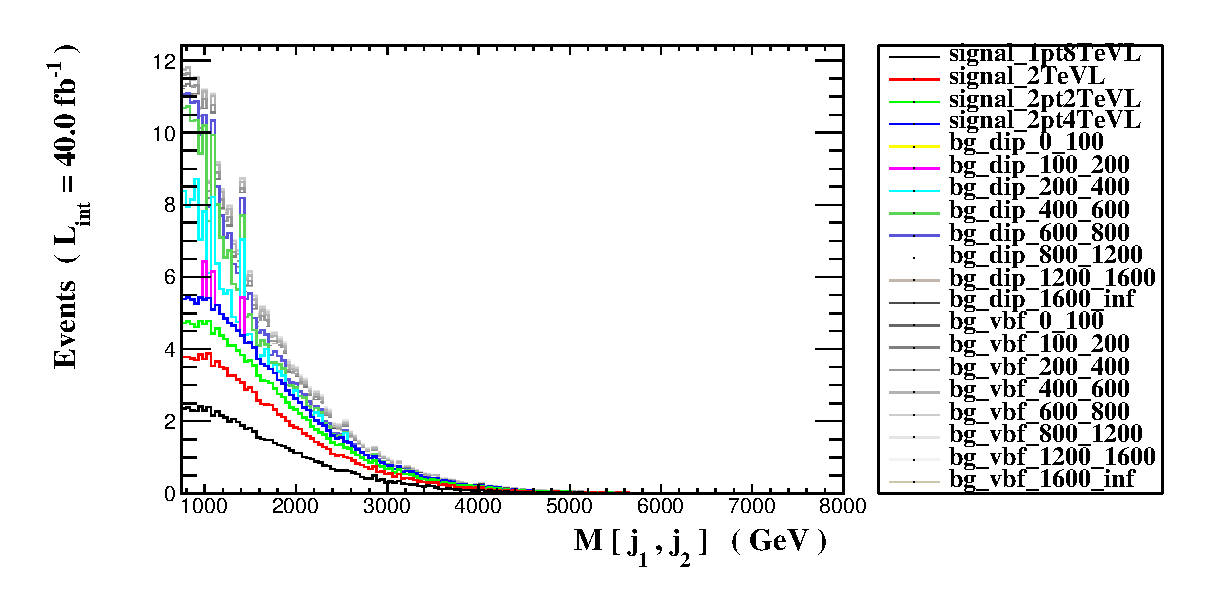
\includegraphics[scale=0.45]{selection_7.eps}\\
\caption{   }
  \end{center}
\end{figure}
      \newpage
\subsection{ Histogram 9}

\textbf{* Plot: sdETA ( jets[1] jets[2] ) }\\
   \begin{table}[H]
  \begin{center}
    \begin{tabular}{|m{23.0mm}|m{23.0mm}|m{18.0mm}|m{19.0mm}|m{19.0mm}|m{19.0mm}|m{19.0mm}|}
      \hline
      {\cellcolor{yellow}         Dataset}& {\cellcolor{yellow}         Integral}& {\cellcolor{yellow}         Entries per event}& {\cellcolor{yellow}         Mean}& {\cellcolor{yellow}         RMS}& {\cellcolor{yellow}         \% underflow}& {\cellcolor{yellow}         \% overflow}\\
      \hline
      {\cellcolor{white}         signal\_1pt8tevl}& {\cellcolor{white}         71.6}& {\cellcolor{white}         1.0}& {\cellcolor{white}         -0.00209236}& {\cellcolor{white}         4.622}& {\cellcolor{red}         50.06}& {\cellcolor{red}         0.0}\\
      \hline
      {\cellcolor{white}         signal\_2tevl}& {\cellcolor{white}         44.7}& {\cellcolor{white}         1.0}& {\cellcolor{white}         -0.0019025}& {\cellcolor{white}         4.69}& {\cellcolor{red}         50.04}& {\cellcolor{red}         0.0}\\
      \hline
      {\cellcolor{white}         signal\_2pt2tevl}& {\cellcolor{white}         29.7}& {\cellcolor{white}         1.0}& {\cellcolor{white}         -0.0403278}& {\cellcolor{white}         4.739}& {\cellcolor{red}         50.38}& {\cellcolor{red}         0.0}\\
      \hline
      {\cellcolor{white}         signal\_2pt4tevl}& {\cellcolor{white}         20.5}& {\cellcolor{white}         1.0}& {\cellcolor{white}         -0.00651616}& {\cellcolor{white}         4.76}& {\cellcolor{red}         50.09}& {\cellcolor{red}         0.0}\\
      \hline
      {\cellcolor{white}         bg\_dip\_0\_100}& {\cellcolor{white}         0.0 +/\-- 0.0}& {\cellcolor{white}         0.}& {\cellcolor{white}         0.0}& {\cellcolor{white}         0.0}& {\cellcolor{green}         0.0}& {\cellcolor{green}         0.0}\\
      \hline
      {\cellcolor{white}         bg\_dip\_100\_200}& {\cellcolor{white}         3.16}& {\cellcolor{white}         1.0}& {\cellcolor{white}         1.51032}& {\cellcolor{white}         5.585}& {\cellcolor{red}         33.38}& {\cellcolor{red}         0.0}\\
      \hline
      {\cellcolor{white}         bg\_dip\_200\_400}& {\cellcolor{white}         25.8}& {\cellcolor{white}         1.0}& {\cellcolor{white}         -0.308501}& {\cellcolor{white}         4.231}& {\cellcolor{red}         54.46}& {\cellcolor{red}         0.0}\\
      \hline
      {\cellcolor{white}         bg\_dip\_400\_600}& {\cellcolor{white}         29.4}& {\cellcolor{white}         1.0}& {\cellcolor{white}         0.0273657}& {\cellcolor{white}         3.639}& {\cellcolor{red}         50.0}& {\cellcolor{red}         0.0}\\
      \hline
      {\cellcolor{white}         bg\_dip\_600\_800}& {\cellcolor{white}         11.9}& {\cellcolor{white}         1.0}& {\cellcolor{white}         -0.10035}& {\cellcolor{white}         3.454}& {\cellcolor{red}         51.48}& {\cellcolor{red}         0.0}\\
      \hline
      {\cellcolor{white}         bg\_dip\_800\_1200}& {\cellcolor{white}         6.14}& {\cellcolor{white}         1.0}& {\cellcolor{white}         0.0462649}& {\cellcolor{white}         3.324}& {\cellcolor{red}         49.19}& {\cellcolor{red}         0.0}\\
      \hline
      {\cellcolor{white}         bg\_dip\_1200\_1600}& {\cellcolor{white}         0.83}& {\cellcolor{white}         1.0}& {\cellcolor{white}         -0.10124}& {\cellcolor{white}         3.147}& {\cellcolor{red}         51.92}& {\cellcolor{red}         0.0}\\
      \hline
      {\cellcolor{white}         bg\_dip\_1600\_inf}& {\cellcolor{white}         0.132}& {\cellcolor{white}         1.0}& {\cellcolor{white}         0.155168}& {\cellcolor{white}         3.003}& {\cellcolor{red}         47.46}& {\cellcolor{red}         0.0}\\
      \hline
      {\cellcolor{white}         bg\_vbf\_0\_100}& {\cellcolor{white}         0.0486}& {\cellcolor{white}         1.0}& {\cellcolor{white}         -0.174236}& {\cellcolor{white}         6.403}& {\cellcolor{red}         50.0}& {\cellcolor{red}         0.0}\\
      \hline
      {\cellcolor{white}         bg\_vbf\_100\_200}& {\cellcolor{white}         1.16}& {\cellcolor{white}         1.0}& {\cellcolor{white}         0.457753}& {\cellcolor{white}         5.752}& {\cellcolor{red}         46.55}& {\cellcolor{red}         0.0}\\
      \hline
      {\cellcolor{white}         bg\_vbf\_200\_400}& {\cellcolor{white}         6.68}& {\cellcolor{white}         1.0}& {\cellcolor{white}         -0.0210876}& {\cellcolor{white}         4.873}& {\cellcolor{red}         50.04}& {\cellcolor{red}         0.0}\\
      \hline
      {\cellcolor{white}         bg\_vbf\_400\_600}& {\cellcolor{white}         6.68}& {\cellcolor{white}         1.0}& {\cellcolor{white}         -0.0753178}& {\cellcolor{white}         4.189}& {\cellcolor{red}         50.97}& {\cellcolor{red}         0.0}\\
      \hline
      {\cellcolor{white}         bg\_vbf\_600\_800}& {\cellcolor{white}         3.03}& {\cellcolor{white}         1.0}& {\cellcolor{white}         -0.00531706}& {\cellcolor{white}         3.854}& {\cellcolor{red}         50.13}& {\cellcolor{red}         0.0}\\
      \hline
      {\cellcolor{white}         bg\_vbf\_800\_1200}& {\cellcolor{white}         1.58}& {\cellcolor{white}         1.0}& {\cellcolor{white}         -0.0630546}& {\cellcolor{white}         3.582}& {\cellcolor{red}         50.81}& {\cellcolor{red}         0.0}\\
      \hline
      {\cellcolor{white}         bg\_vbf\_1200\_1600}& {\cellcolor{white}         0.236}& {\cellcolor{white}         1.0}& {\cellcolor{white}         -0.0646725}& {\cellcolor{white}         3.319}& {\cellcolor{red}         50.8}& {\cellcolor{red}         0.0}\\
      \hline
      {\cellcolor{white}         bg\_vbf\_1600\_inf}& {\cellcolor{white}         0.0444}& {\cellcolor{white}         1.0}& {\cellcolor{white}         0.116643}& {\cellcolor{white}         3.131}& {\cellcolor{red}         48.21}& {\cellcolor{red}         0.0}\\
\hline
    \end{tabular}
  \end{center}
\end{table}

\begin{figure}[H]
  \begin{center}
    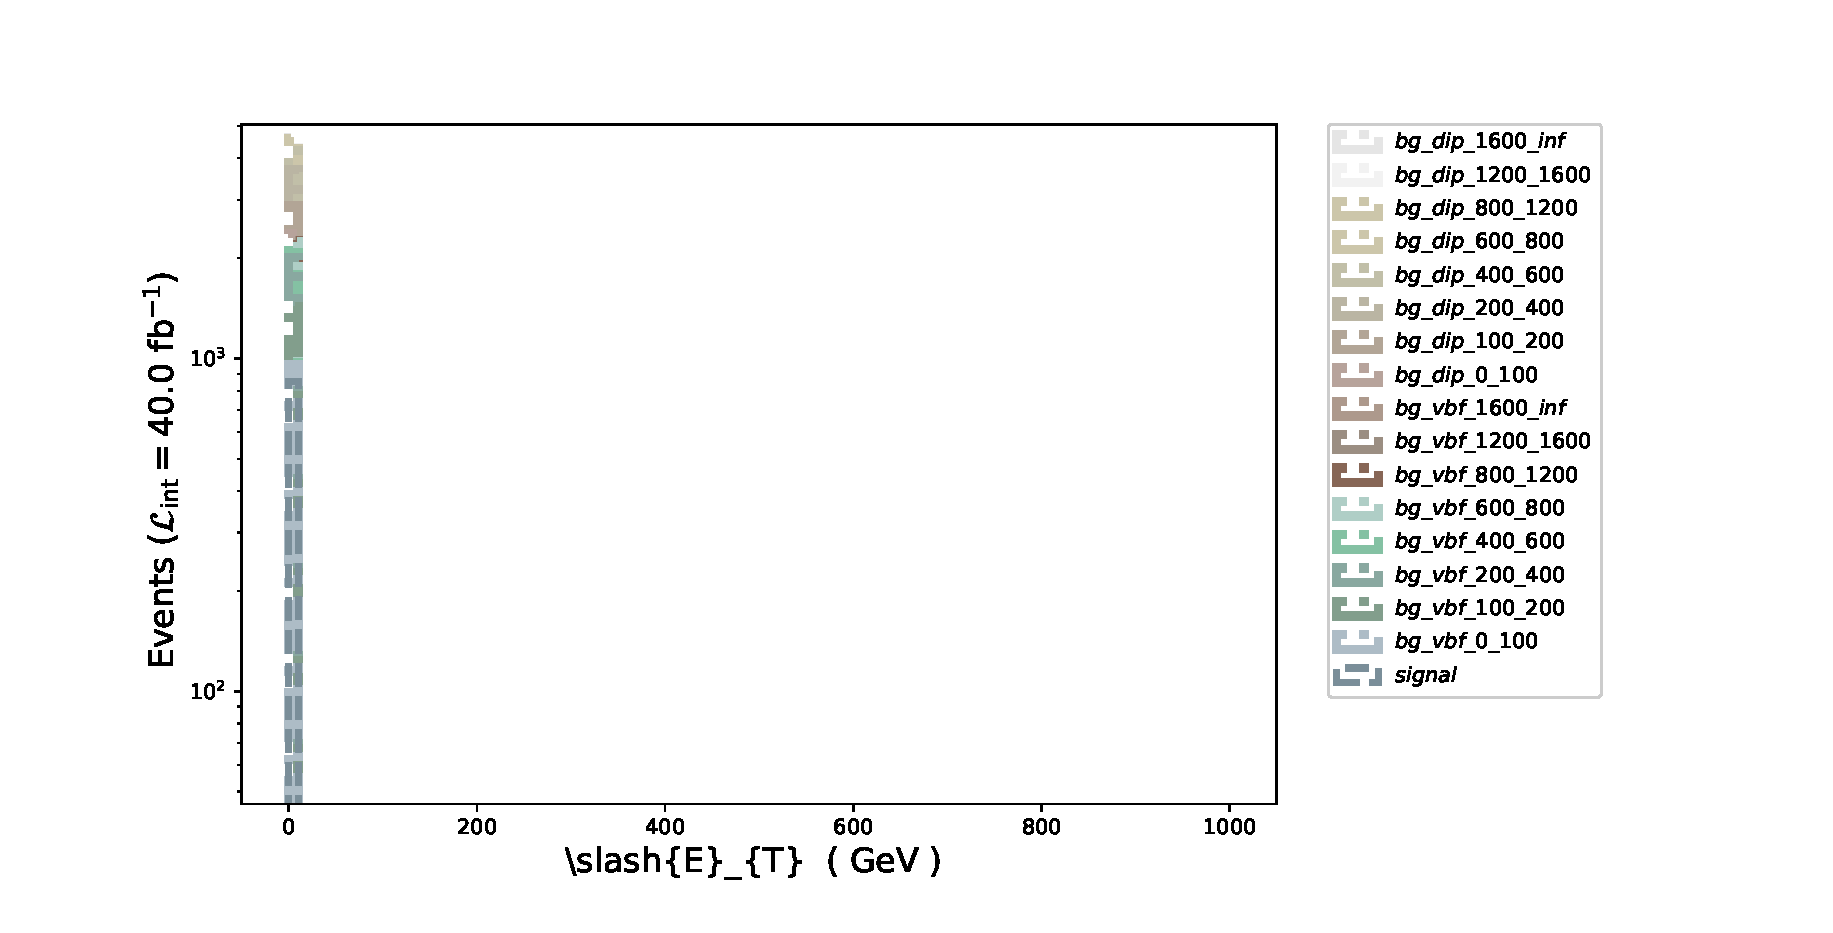
\includegraphics[scale=0.45]{selection_8.eps}\\
\caption{   }
  \end{center}
\end{figure}
      \newpage
\subsection{ Histogram 10}

\textbf{* Plot: M ( a[1] a[2] ) }\\
   \begin{table}[H]
  \begin{center}
    \begin{tabular}{|m{23.0mm}|m{23.0mm}|m{18.0mm}|m{19.0mm}|m{19.0mm}|m{19.0mm}|m{19.0mm}|}
      \hline
      {\cellcolor{yellow}         Dataset}& {\cellcolor{yellow}         Integral}& {\cellcolor{yellow}         Entries per event}& {\cellcolor{yellow}         Mean}& {\cellcolor{yellow}         RMS}& {\cellcolor{yellow}         \% underflow}& {\cellcolor{yellow}         \% overflow}\\
      \hline
      {\cellcolor{white}         signal\_1pt8tevl}& {\cellcolor{white}         71.6}& {\cellcolor{white}         1.0}& {\cellcolor{white}         1440.41}& {\cellcolor{white}         804.8}& {\cellcolor{green}         0.0}& {\cellcolor{green}         1.282}\\
      \hline
      {\cellcolor{white}         signal\_2tevl}& {\cellcolor{white}         44.7}& {\cellcolor{white}         1.0}& {\cellcolor{white}         1452.91}& {\cellcolor{white}         814.5}& {\cellcolor{green}         0.0}& {\cellcolor{green}         1.3}\\
      \hline
      {\cellcolor{white}         signal\_2pt2tevl}& {\cellcolor{white}         29.7}& {\cellcolor{white}         1.0}& {\cellcolor{white}         1458.99}& {\cellcolor{white}         818.6}& {\cellcolor{green}         0.0}& {\cellcolor{green}         1.395}\\
      \hline
      {\cellcolor{white}         signal\_2pt4tevl}& {\cellcolor{white}         20.5}& {\cellcolor{white}         1.0}& {\cellcolor{white}         1467.75}& {\cellcolor{white}         823.2}& {\cellcolor{green}         0.0}& {\cellcolor{green}         1.422}\\
      \hline
      {\cellcolor{white}         bg\_dip\_0\_100}& {\cellcolor{white}         0.0 +/\-- 0.0}& {\cellcolor{white}         0.}& {\cellcolor{white}         0.0}& {\cellcolor{white}         0.0}& {\cellcolor{green}         0.0}& {\cellcolor{green}         0.0}\\
      \hline
      {\cellcolor{white}         bg\_dip\_100\_200}& {\cellcolor{white}         3.16}& {\cellcolor{white}         1.0}& {\cellcolor{white}         674.287}& {\cellcolor{white}         36.08}& {\cellcolor{green}         0.0}& {\cellcolor{green}         0.0}\\
      \hline
      {\cellcolor{white}         bg\_dip\_200\_400}& {\cellcolor{white}         25.8}& {\cellcolor{white}         1.0}& {\cellcolor{white}         806.444}& {\cellcolor{white}         369.4}& {\cellcolor{green}         0.0}& {\cellcolor{green}         0.0}\\
      \hline
      {\cellcolor{white}         bg\_dip\_400\_600}& {\cellcolor{white}         29.4}& {\cellcolor{white}         1.0}& {\cellcolor{white}         757.536}& {\cellcolor{white}         302.7}& {\cellcolor{green}         0.0}& {\cellcolor{green}         0.0}\\
      \hline
      {\cellcolor{white}         bg\_dip\_600\_800}& {\cellcolor{white}         11.9}& {\cellcolor{white}         1.0}& {\cellcolor{white}         794.656}& {\cellcolor{white}         340.2}& {\cellcolor{green}         0.0}& {\cellcolor{green}         0.0}\\
      \hline
      {\cellcolor{white}         bg\_dip\_800\_1200}& {\cellcolor{white}         6.14}& {\cellcolor{white}         1.0}& {\cellcolor{white}         817.407}& {\cellcolor{white}         345.6}& {\cellcolor{green}         0.0}& {\cellcolor{green}         0.0}\\
      \hline
      {\cellcolor{white}         bg\_dip\_1200\_1600}& {\cellcolor{white}         0.83}& {\cellcolor{white}         1.0}& {\cellcolor{white}         857.308}& {\cellcolor{white}         368.7}& {\cellcolor{green}         0.0}& {\cellcolor{green}         0.0}\\
      \hline
      {\cellcolor{white}         bg\_dip\_1600\_inf}& {\cellcolor{white}         0.132}& {\cellcolor{white}         1.0}& {\cellcolor{white}         894.427}& {\cellcolor{white}         438.3}& {\cellcolor{green}         0.0}& {\cellcolor{green}         0.0}\\
      \hline
      {\cellcolor{white}         bg\_vbf\_0\_100}& {\cellcolor{white}         0.0486}& {\cellcolor{white}         1.0}& {\cellcolor{white}         999.408}& {\cellcolor{white}         375.3}& {\cellcolor{green}         0.0}& {\cellcolor{green}         0.0}\\
      \hline
      {\cellcolor{white}         bg\_vbf\_100\_200}& {\cellcolor{white}         1.16}& {\cellcolor{white}         1.0}& {\cellcolor{white}         847.835}& {\cellcolor{white}         279.9}& {\cellcolor{green}         0.0}& {\cellcolor{green}         0.0}\\
      \hline
      {\cellcolor{white}         bg\_vbf\_200\_400}& {\cellcolor{white}         6.68}& {\cellcolor{white}         1.0}& {\cellcolor{white}         801.713}& {\cellcolor{white}         329.2}& {\cellcolor{green}         0.0}& {\cellcolor{green}         0.0}\\
      \hline
      {\cellcolor{white}         bg\_vbf\_400\_600}& {\cellcolor{white}         6.68}& {\cellcolor{white}         1.0}& {\cellcolor{white}         752.011}& {\cellcolor{white}         284.8}& {\cellcolor{green}         0.0}& {\cellcolor{green}         0.0}\\
      \hline
      {\cellcolor{white}         bg\_vbf\_600\_800}& {\cellcolor{white}         3.03}& {\cellcolor{white}         1.0}& {\cellcolor{white}         766.09}& {\cellcolor{white}         289.0}& {\cellcolor{green}         0.0}& {\cellcolor{green}         0.0}\\
      \hline
      {\cellcolor{white}         bg\_vbf\_800\_1200}& {\cellcolor{white}         1.58}& {\cellcolor{white}         1.0}& {\cellcolor{white}         787.04}& {\cellcolor{white}         304.8}& {\cellcolor{green}         0.0}& {\cellcolor{green}         0.0}\\
      \hline
      {\cellcolor{white}         bg\_vbf\_1200\_1600}& {\cellcolor{white}         0.236}& {\cellcolor{white}         1.0}& {\cellcolor{white}         805.651}& {\cellcolor{white}         327.2}& {\cellcolor{green}         0.0}& {\cellcolor{green}         0.009129}\\
      \hline
      {\cellcolor{white}         bg\_vbf\_1600\_inf}& {\cellcolor{white}         0.0444}& {\cellcolor{white}         1.0}& {\cellcolor{white}         833.17}& {\cellcolor{white}         363.6}& {\cellcolor{green}         0.0}& {\cellcolor{green}         0.06398}\\
\hline
    \end{tabular}
  \end{center}
\end{table}

\begin{figure}[H]
  \begin{center}
    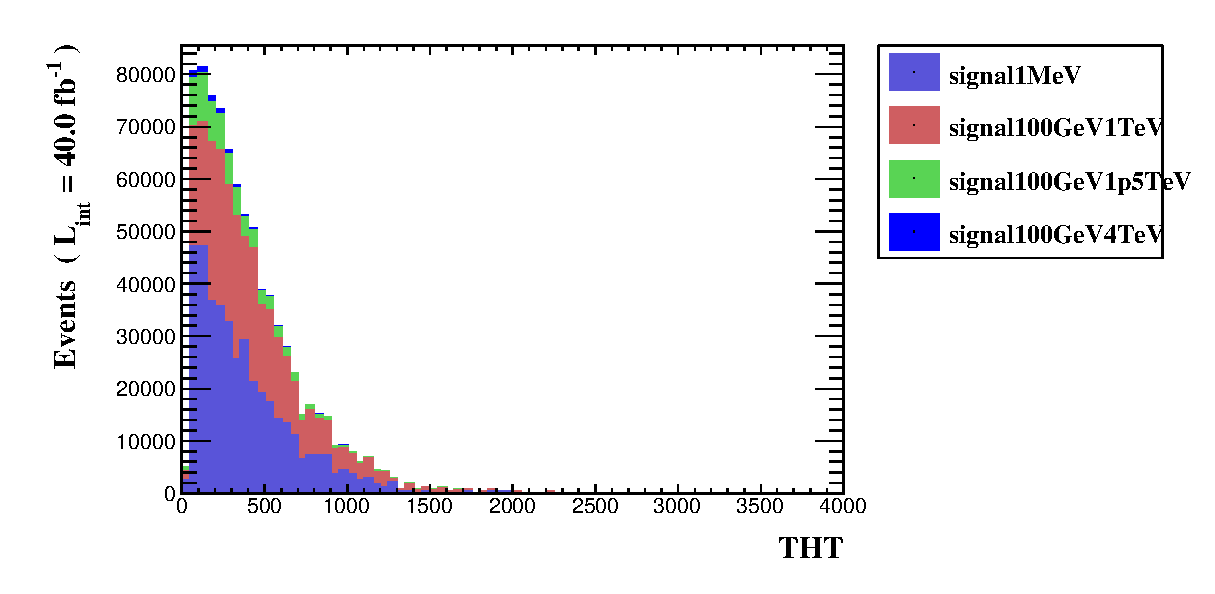
\includegraphics[scale=0.45]{selection_9.eps}\\
\caption{   }
  \end{center}
\end{figure}
      \newpage
\subsection{ Histogram 11}

\textbf{* Plot: PT ( a[1] ) }\\
   \begin{table}[H]
  \begin{center}
    \begin{tabular}{|m{23.0mm}|m{23.0mm}|m{18.0mm}|m{19.0mm}|m{19.0mm}|m{19.0mm}|m{19.0mm}|}
      \hline
      {\cellcolor{yellow}         Dataset}& {\cellcolor{yellow}         Integral}& {\cellcolor{yellow}         Entries per event}& {\cellcolor{yellow}         Mean}& {\cellcolor{yellow}         RMS}& {\cellcolor{yellow}         \% underflow}& {\cellcolor{yellow}         \% overflow}\\
      \hline
      {\cellcolor{white}         signal\_1pt8tevl}& {\cellcolor{white}         71.6}& {\cellcolor{white}         1.0}& {\cellcolor{white}         759.899}& {\cellcolor{white}         377.4}& {\cellcolor{green}         0.0}& {\cellcolor{green}         1.082}\\
      \hline
      {\cellcolor{white}         signal\_2tevl}& {\cellcolor{white}         44.7}& {\cellcolor{white}         1.0}& {\cellcolor{white}         760.681}& {\cellcolor{white}         378.3}& {\cellcolor{green}         0.0}& {\cellcolor{green}         1.008}\\
      \hline
      {\cellcolor{white}         signal\_2pt2tevl}& {\cellcolor{white}         29.7}& {\cellcolor{white}         1.0}& {\cellcolor{white}         759.161}& {\cellcolor{white}         380.0}& {\cellcolor{green}         0.0}& {\cellcolor{green}         1.093}\\
      \hline
      {\cellcolor{white}         signal\_2pt4tevl}& {\cellcolor{white}         20.5}& {\cellcolor{white}         1.0}& {\cellcolor{white}         758.578}& {\cellcolor{white}         383.3}& {\cellcolor{green}         0.0}& {\cellcolor{green}         1.123}\\
      \hline
      {\cellcolor{white}         bg\_dip\_0\_100}& {\cellcolor{white}         0.0 +/\-- 0.0}& {\cellcolor{white}         0.}& {\cellcolor{white}         0.0}& {\cellcolor{white}         0.0}& {\cellcolor{green}         0.0}& {\cellcolor{green}         0.0}\\
      \hline
      {\cellcolor{white}         bg\_dip\_100\_200}& {\cellcolor{white}         3.16}& {\cellcolor{white}         1.0}& {\cellcolor{white}         327.174}& {\cellcolor{white}         7.434}& {\cellcolor{green}         0.0}& {\cellcolor{green}         0.0}\\
      \hline
      {\cellcolor{white}         bg\_dip\_200\_400}& {\cellcolor{white}         25.8}& {\cellcolor{white}         1.0}& {\cellcolor{white}         400.151}& {\cellcolor{white}         82.89}& {\cellcolor{green}         0.0}& {\cellcolor{green}         0.0}\\
      \hline
      {\cellcolor{white}         bg\_dip\_400\_600}& {\cellcolor{white}         29.4}& {\cellcolor{white}         1.0}& {\cellcolor{white}         453.621}& {\cellcolor{white}         116.0}& {\cellcolor{green}         0.0}& {\cellcolor{green}         0.0}\\
      \hline
      {\cellcolor{white}         bg\_dip\_600\_800}& {\cellcolor{white}         11.9}& {\cellcolor{white}         1.0}& {\cellcolor{white}         556.513}& {\cellcolor{white}         168.6}& {\cellcolor{green}         0.0}& {\cellcolor{green}         0.0}\\
      \hline
      {\cellcolor{white}         bg\_dip\_800\_1200}& {\cellcolor{white}         6.14}& {\cellcolor{white}         1.0}& {\cellcolor{white}         681.169}& {\cellcolor{white}         251.5}& {\cellcolor{green}         0.0}& {\cellcolor{green}         0.04611}\\
      \hline
      {\cellcolor{white}         bg\_dip\_1200\_1600}& {\cellcolor{white}         0.83}& {\cellcolor{white}         1.0}& {\cellcolor{white}         836.694}& {\cellcolor{white}         405.5}& {\cellcolor{green}         0.0}& {\cellcolor{green}         0.0}\\
      \hline
      {\cellcolor{white}         bg\_dip\_1600\_inf}& {\cellcolor{white}         0.132}& {\cellcolor{white}         1.0}& {\cellcolor{white}         896.187}& {\cellcolor{white}         576.0}& {\cellcolor{green}         0.0}& {\cellcolor{green}         3.979}\\
      \hline
      {\cellcolor{white}         bg\_vbf\_0\_100}& {\cellcolor{white}         0.0486}& {\cellcolor{white}         1.0}& {\cellcolor{white}         379.899}& {\cellcolor{white}         64.59}& {\cellcolor{green}         0.0}& {\cellcolor{green}         0.0}\\
      \hline
      {\cellcolor{white}         bg\_vbf\_100\_200}& {\cellcolor{white}         1.16}& {\cellcolor{white}         1.0}& {\cellcolor{white}         373.902}& {\cellcolor{white}         77.67}& {\cellcolor{green}         0.0}& {\cellcolor{green}         0.0}\\
      \hline
      {\cellcolor{white}         bg\_vbf\_200\_400}& {\cellcolor{white}         6.68}& {\cellcolor{white}         1.0}& {\cellcolor{white}         392.202}& {\cellcolor{white}         92.25}& {\cellcolor{green}         0.0}& {\cellcolor{green}         0.0}\\
      \hline
      {\cellcolor{white}         bg\_vbf\_400\_600}& {\cellcolor{white}         6.68}& {\cellcolor{white}         1.0}& {\cellcolor{white}         437.392}& {\cellcolor{white}         113.3}& {\cellcolor{green}         0.0}& {\cellcolor{green}         0.0}\\
      \hline
      {\cellcolor{white}         bg\_vbf\_600\_800}& {\cellcolor{white}         3.03}& {\cellcolor{white}         1.0}& {\cellcolor{white}         511.989}& {\cellcolor{white}         149.4}& {\cellcolor{green}         0.0}& {\cellcolor{green}         0.0}\\
      \hline
      {\cellcolor{white}         bg\_vbf\_800\_1200}& {\cellcolor{white}         1.58}& {\cellcolor{white}         1.0}& {\cellcolor{white}         630.881}& {\cellcolor{white}         223.5}& {\cellcolor{green}         0.0}& {\cellcolor{green}         0.0}\\
      \hline
      {\cellcolor{white}         bg\_vbf\_1200\_1600}& {\cellcolor{white}         0.236}& {\cellcolor{white}         1.0}& {\cellcolor{white}         793.987}& {\cellcolor{white}         347.0}& {\cellcolor{green}         0.0}& {\cellcolor{green}         0.03651}\\
      \hline
      {\cellcolor{white}         bg\_vbf\_1600\_inf}& {\cellcolor{white}         0.0444}& {\cellcolor{white}         1.0}& {\cellcolor{white}         957.485}& {\cellcolor{white}         518.9}& {\cellcolor{green}         0.0}& {\cellcolor{green}         2.106}\\
\hline
    \end{tabular}
  \end{center}
\end{table}

\begin{figure}[H]
  \begin{center}
    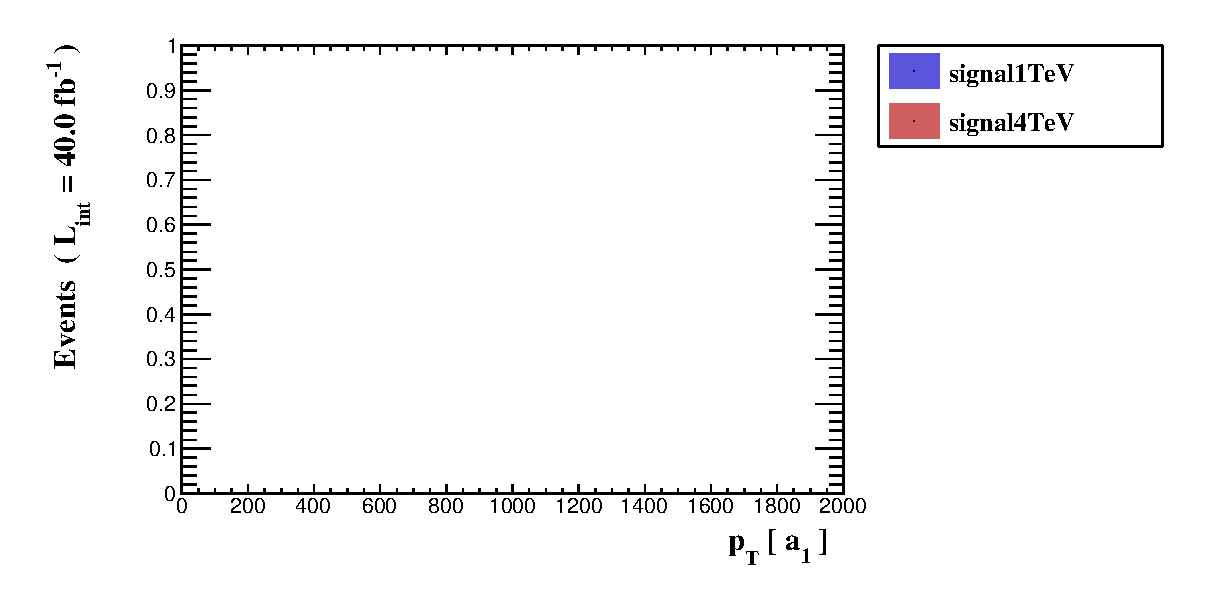
\includegraphics[scale=0.45]{selection_10.eps}\\
\caption{   }
  \end{center}
\end{figure}
      \newpage
\subsection{ Histogram 12}

\textbf{* Plot: PT ( a[2] ) }\\
   \begin{table}[H]
  \begin{center}
    \begin{tabular}{|m{23.0mm}|m{23.0mm}|m{18.0mm}|m{19.0mm}|m{19.0mm}|m{19.0mm}|m{19.0mm}|}
      \hline
      {\cellcolor{yellow}         Dataset}& {\cellcolor{yellow}         Integral}& {\cellcolor{yellow}         Entries per event}& {\cellcolor{yellow}         Mean}& {\cellcolor{yellow}         RMS}& {\cellcolor{yellow}         \% underflow}& {\cellcolor{yellow}         \% overflow}\\
      \hline
      {\cellcolor{white}         signal\_1pt8tevl}& {\cellcolor{white}         71.6}& {\cellcolor{white}         1.0}& {\cellcolor{white}         513.442}& {\cellcolor{white}         347.0}& {\cellcolor{green}         0.0}& {\cellcolor{green}         0.4596}\\
      \hline
      {\cellcolor{white}         signal\_2tevl}& {\cellcolor{white}         44.7}& {\cellcolor{white}         1.0}& {\cellcolor{white}         518.547}& {\cellcolor{white}         351.9}& {\cellcolor{green}         0.0}& {\cellcolor{green}         0.4301}\\
      \hline
      {\cellcolor{white}         signal\_2pt2tevl}& {\cellcolor{white}         29.7}& {\cellcolor{white}         1.0}& {\cellcolor{white}         520.349}& {\cellcolor{white}         352.1}& {\cellcolor{green}         0.0}& {\cellcolor{green}         0.4284}\\
      \hline
      {\cellcolor{white}         signal\_2pt4tevl}& {\cellcolor{white}         20.5}& {\cellcolor{white}         1.0}& {\cellcolor{white}         521.952}& {\cellcolor{white}         355.0}& {\cellcolor{green}         0.0}& {\cellcolor{green}         0.4715}\\
      \hline
      {\cellcolor{white}         bg\_dip\_0\_100}& {\cellcolor{white}         0.0 +/\-- 0.0}& {\cellcolor{white}         0.}& {\cellcolor{white}         0.0}& {\cellcolor{white}         0.0}& {\cellcolor{green}         0.0}& {\cellcolor{green}         0.0}\\
      \hline
      {\cellcolor{white}         bg\_dip\_100\_200}& {\cellcolor{white}         3.16}& {\cellcolor{white}         1.0}& {\cellcolor{white}         253.391}& {\cellcolor{white}         44.39}& {\cellcolor{green}         0.0}& {\cellcolor{green}         0.0}\\
      \hline
      {\cellcolor{white}         bg\_dip\_200\_400}& {\cellcolor{white}         25.8}& {\cellcolor{white}         1.0}& {\cellcolor{white}         191.937}& {\cellcolor{white}         101.6}& {\cellcolor{green}         0.0}& {\cellcolor{green}         0.0}\\
      \hline
      {\cellcolor{white}         bg\_dip\_400\_600}& {\cellcolor{white}         29.4}& {\cellcolor{white}         1.0}& {\cellcolor{white}         141.385}& {\cellcolor{white}         100.6}& {\cellcolor{green}         0.0}& {\cellcolor{green}         0.0}\\
      \hline
      {\cellcolor{white}         bg\_dip\_600\_800}& {\cellcolor{white}         11.9}& {\cellcolor{white}         1.0}& {\cellcolor{white}         138.099}& {\cellcolor{white}         111.8}& {\cellcolor{green}         0.0}& {\cellcolor{green}         0.0}\\
      \hline
      {\cellcolor{white}         bg\_dip\_800\_1200}& {\cellcolor{white}         6.14}& {\cellcolor{white}         1.0}& {\cellcolor{white}         133.82}& {\cellcolor{white}         114.3}& {\cellcolor{green}         0.0}& {\cellcolor{green}         0.0}\\
      \hline
      {\cellcolor{white}         bg\_dip\_1200\_1600}& {\cellcolor{white}         0.83}& {\cellcolor{white}         1.0}& {\cellcolor{white}         124.476}& {\cellcolor{white}         117.4}& {\cellcolor{green}         0.0}& {\cellcolor{green}         0.0}\\
      \hline
      {\cellcolor{white}         bg\_dip\_1600\_inf}& {\cellcolor{white}         0.132}& {\cellcolor{white}         1.0}& {\cellcolor{white}         133.187}& {\cellcolor{white}         137.3}& {\cellcolor{green}         0.0}& {\cellcolor{green}         0.0}\\
      \hline
      {\cellcolor{white}         bg\_vbf\_0\_100}& {\cellcolor{white}         0.0486}& {\cellcolor{white}         1.0}& {\cellcolor{white}         359.837}& {\cellcolor{white}         74.21}& {\cellcolor{green}         0.0}& {\cellcolor{green}         0.0}\\
      \hline
      {\cellcolor{white}         bg\_vbf\_100\_200}& {\cellcolor{white}         1.16}& {\cellcolor{white}         1.0}& {\cellcolor{white}         285.217}& {\cellcolor{white}         94.57}& {\cellcolor{green}         0.0}& {\cellcolor{green}         0.0}\\
      \hline
      {\cellcolor{white}         bg\_vbf\_200\_400}& {\cellcolor{white}         6.68}& {\cellcolor{white}         1.0}& {\cellcolor{white}         209.279}& {\cellcolor{white}         119.1}& {\cellcolor{green}         0.0}& {\cellcolor{green}         0.0}\\
      \hline
      {\cellcolor{white}         bg\_vbf\_400\_600}& {\cellcolor{white}         6.68}& {\cellcolor{white}         1.0}& {\cellcolor{white}         163.048}& {\cellcolor{white}         118.3}& {\cellcolor{green}         0.0}& {\cellcolor{green}         0.0}\\
      \hline
      {\cellcolor{white}         bg\_vbf\_600\_800}& {\cellcolor{white}         3.03}& {\cellcolor{white}         1.0}& {\cellcolor{white}         160.555}& {\cellcolor{white}         112.8}& {\cellcolor{green}         0.0}& {\cellcolor{green}         0.0}\\
      \hline
      {\cellcolor{white}         bg\_vbf\_800\_1200}& {\cellcolor{white}         1.58}& {\cellcolor{white}         1.0}& {\cellcolor{white}         166.84}& {\cellcolor{white}         124.1}& {\cellcolor{green}         0.0}& {\cellcolor{green}         0.0}\\
      \hline
      {\cellcolor{white}         bg\_vbf\_1200\_1600}& {\cellcolor{white}         0.236}& {\cellcolor{white}         1.0}& {\cellcolor{white}         171.935}& {\cellcolor{white}         136.6}& {\cellcolor{green}         0.0}& {\cellcolor{green}         0.0}\\
      \hline
      {\cellcolor{white}         bg\_vbf\_1600\_inf}& {\cellcolor{white}         0.0444}& {\cellcolor{white}         1.0}& {\cellcolor{white}         183.125}& {\cellcolor{white}         156.6}& {\cellcolor{green}         0.0}& {\cellcolor{green}         0.0}\\
\hline
    \end{tabular}
  \end{center}
\end{table}

\begin{figure}[H]
  \begin{center}
    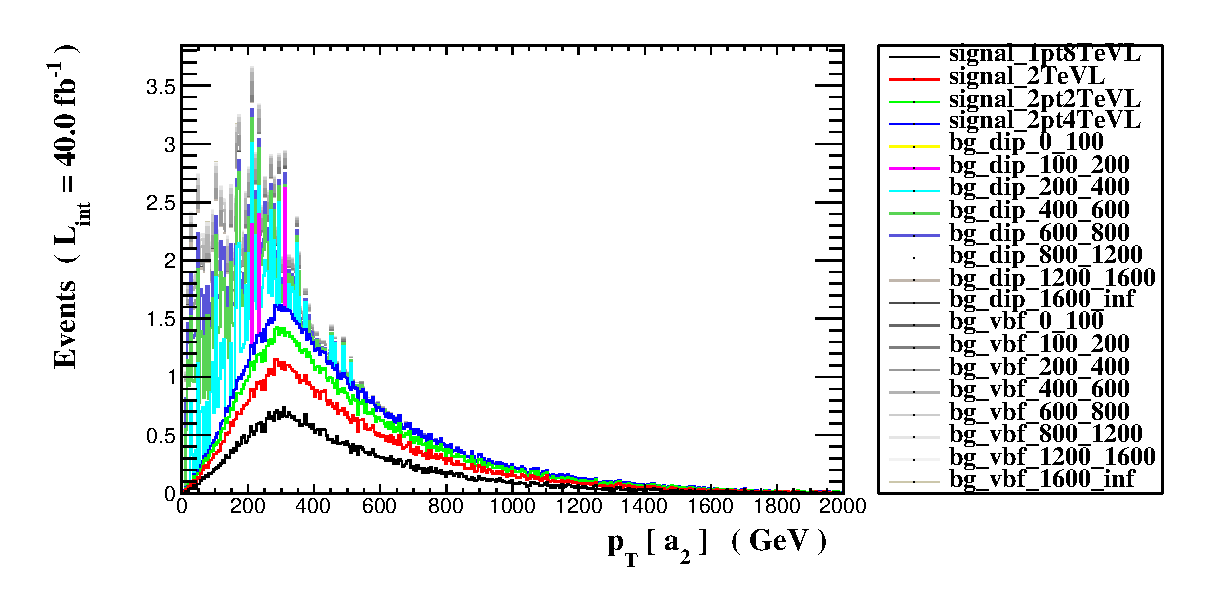
\includegraphics[scale=0.45]{selection_11.eps}\\
\caption{   }
  \end{center}
\end{figure}
      \newpage
\subsection{ Histogram 13}

\textbf{* Plot: THT}\\
   \begin{table}[H]
  \begin{center}
    \begin{tabular}{|m{23.0mm}|m{23.0mm}|m{18.0mm}|m{19.0mm}|m{19.0mm}|m{19.0mm}|m{19.0mm}|}
      \hline
      {\cellcolor{yellow}         Dataset}& {\cellcolor{yellow}         Integral}& {\cellcolor{yellow}         Entries per event}& {\cellcolor{yellow}         Mean}& {\cellcolor{yellow}         RMS}& {\cellcolor{yellow}         \% underflow}& {\cellcolor{yellow}         \% overflow}\\
      \hline
      {\cellcolor{white}         signal\_1pt8tevl}& {\cellcolor{white}         71.6}& {\cellcolor{white}         1.0}& {\cellcolor{white}         523.292}& {\cellcolor{white}         343.8}& {\cellcolor{green}         0.0}& {\cellcolor{green}         0.0}\\
      \hline
      {\cellcolor{white}         signal\_2tevl}& {\cellcolor{white}         44.7}& {\cellcolor{white}         1.0}& {\cellcolor{white}         507.702}& {\cellcolor{white}         334.1}& {\cellcolor{green}         0.0}& {\cellcolor{green}         0.0}\\
      \hline
      {\cellcolor{white}         signal\_2pt2tevl}& {\cellcolor{white}         29.7}& {\cellcolor{white}         1.0}& {\cellcolor{white}         498.796}& {\cellcolor{white}         330.9}& {\cellcolor{green}         0.0}& {\cellcolor{green}         0.0}\\
      \hline
      {\cellcolor{white}         signal\_2pt4tevl}& {\cellcolor{white}         20.5}& {\cellcolor{white}         1.0}& {\cellcolor{white}         490.831}& {\cellcolor{white}         326.9}& {\cellcolor{green}         0.0}& {\cellcolor{green}         0.0}\\
      \hline
      {\cellcolor{white}         bg\_dip\_0\_100}& {\cellcolor{white}         0.0 +/\-- 0.0}& {\cellcolor{white}         0.}& {\cellcolor{white}         0.0}& {\cellcolor{white}         0.0}& {\cellcolor{green}         0.0}& {\cellcolor{green}         0.0}\\
      \hline
      {\cellcolor{white}         bg\_dip\_100\_200}& {\cellcolor{white}         3.16}& {\cellcolor{white}         1.0}& {\cellcolor{white}         148.168}& {\cellcolor{white}         37.58}& {\cellcolor{green}         0.0}& {\cellcolor{green}         0.0}\\
      \hline
      {\cellcolor{white}         bg\_dip\_200\_400}& {\cellcolor{white}         25.8}& {\cellcolor{white}         1.0}& {\cellcolor{white}         322.57}& {\cellcolor{white}         51.94}& {\cellcolor{green}         0.0}& {\cellcolor{green}         0.0}\\
      \hline
      {\cellcolor{white}         bg\_dip\_400\_600}& {\cellcolor{white}         29.4}& {\cellcolor{white}         1.0}& {\cellcolor{white}         491.06}& {\cellcolor{white}         56.32}& {\cellcolor{green}         0.0}& {\cellcolor{green}         0.0}\\
      \hline
      {\cellcolor{white}         bg\_dip\_600\_800}& {\cellcolor{white}         11.9}& {\cellcolor{white}         1.0}& {\cellcolor{white}         684.399}& {\cellcolor{white}         55.83}& {\cellcolor{green}         0.0}& {\cellcolor{green}         0.0}\\
      \hline
      {\cellcolor{white}         bg\_dip\_800\_1200}& {\cellcolor{white}         6.14}& {\cellcolor{white}         1.0}& {\cellcolor{white}         935.186}& {\cellcolor{white}         105.9}& {\cellcolor{green}         0.0}& {\cellcolor{green}         0.0}\\
      \hline
      {\cellcolor{white}         bg\_dip\_1200\_1600}& {\cellcolor{white}         0.83}& {\cellcolor{white}         1.0}& {\cellcolor{white}         1339.85}& {\cellcolor{white}         106.6}& {\cellcolor{green}         0.0}& {\cellcolor{green}         0.0}\\
      \hline
      {\cellcolor{white}         bg\_dip\_1600\_inf}& {\cellcolor{white}         0.132}& {\cellcolor{white}         1.0}& {\cellcolor{white}         1838.6}& {\cellcolor{white}         235.7}& {\cellcolor{green}         0.0}& {\cellcolor{green}         0.0}\\
      \hline
      {\cellcolor{white}         bg\_vbf\_0\_100}& {\cellcolor{white}         0.0486}& {\cellcolor{white}         1.0}& {\cellcolor{white}         74.6978}& {\cellcolor{white}         15.53}& {\cellcolor{green}         0.0}& {\cellcolor{green}         0.0}\\
      \hline
      {\cellcolor{white}         bg\_vbf\_100\_200}& {\cellcolor{white}         1.16}& {\cellcolor{white}         1.0}& {\cellcolor{white}         163.344}& {\cellcolor{white}         25.73}& {\cellcolor{green}         0.0}& {\cellcolor{green}         0.0}\\
      \hline
      {\cellcolor{white}         bg\_vbf\_200\_400}& {\cellcolor{white}         6.68}& {\cellcolor{white}         1.0}& {\cellcolor{white}         310.201}& {\cellcolor{white}         55.23}& {\cellcolor{green}         0.0}& {\cellcolor{green}         0.0}\\
      \hline
      {\cellcolor{white}         bg\_vbf\_400\_600}& {\cellcolor{white}         6.68}& {\cellcolor{white}         1.0}& {\cellcolor{white}         489.26}& {\cellcolor{white}         55.92}& {\cellcolor{green}         0.0}& {\cellcolor{green}         0.0}\\
      \hline
      {\cellcolor{white}         bg\_vbf\_600\_800}& {\cellcolor{white}         3.03}& {\cellcolor{white}         1.0}& {\cellcolor{white}         684.802}& {\cellcolor{white}         56.45}& {\cellcolor{green}         0.0}& {\cellcolor{green}         0.0}\\
      \hline
      {\cellcolor{white}         bg\_vbf\_800\_1200}& {\cellcolor{white}         1.58}& {\cellcolor{white}         1.0}& {\cellcolor{white}         938.007}& {\cellcolor{white}         105.1}& {\cellcolor{green}         0.0}& {\cellcolor{green}         0.0}\\
      \hline
      {\cellcolor{white}         bg\_vbf\_1200\_1600}& {\cellcolor{white}         0.236}& {\cellcolor{white}         1.0}& {\cellcolor{white}         1341.72}& {\cellcolor{white}         107.1}& {\cellcolor{green}         0.0}& {\cellcolor{green}         0.0}\\
      \hline
      {\cellcolor{white}         bg\_vbf\_1600\_inf}& {\cellcolor{white}         0.0444}& {\cellcolor{white}         1.0}& {\cellcolor{white}         1815.22}& {\cellcolor{white}         215.1}& {\cellcolor{green}         0.0}& {\cellcolor{green}         0.0}\\
\hline
    \end{tabular}
  \end{center}
\end{table}

\begin{figure}[H]
  \begin{center}
    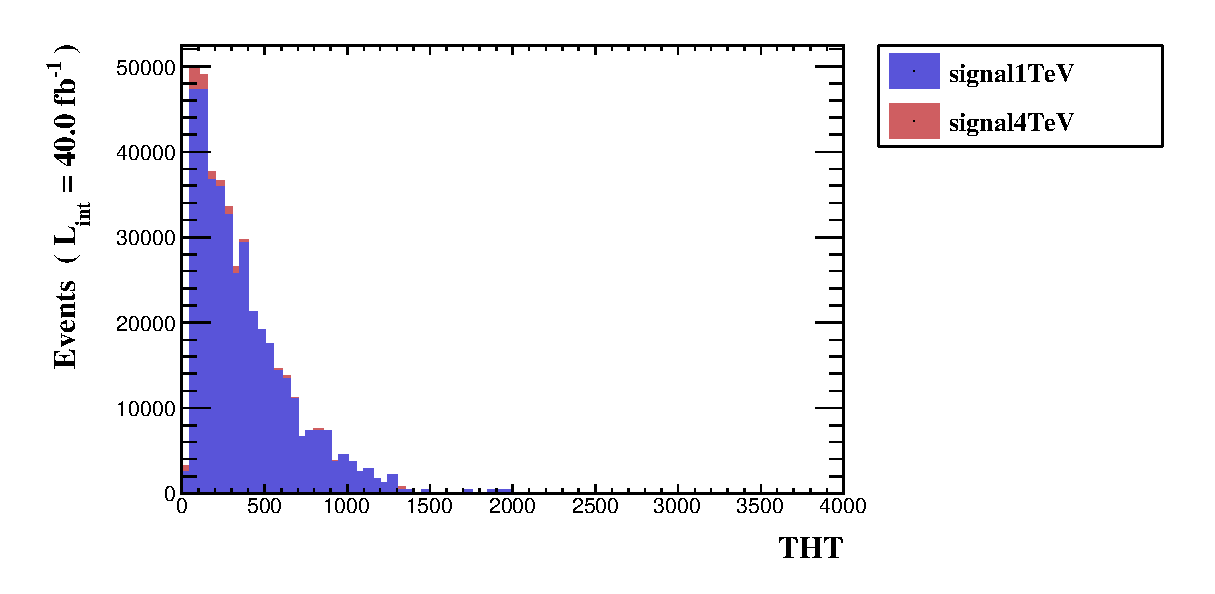
\includegraphics[scale=0.45]{selection_12.eps}\\
\caption{   }
  \end{center}
\end{figure}
      \newpage
\subsection{ Histogram 14}

\textbf{* Plot: MET}\\
   \begin{table}[H]
  \begin{center}
    \begin{tabular}{|m{23.0mm}|m{23.0mm}|m{18.0mm}|m{19.0mm}|m{19.0mm}|m{19.0mm}|m{19.0mm}|}
      \hline
      {\cellcolor{yellow}         Dataset}& {\cellcolor{yellow}         Integral}& {\cellcolor{yellow}         Entries per event}& {\cellcolor{yellow}         Mean}& {\cellcolor{yellow}         RMS}& {\cellcolor{yellow}         \% underflow}& {\cellcolor{yellow}         \% overflow}\\
      \hline
      {\cellcolor{white}         signal\_1pt8tevl}& {\cellcolor{white}         71.6}& {\cellcolor{white}         1.0}& {\cellcolor{white}         1.01393e-08}& {\cellcolor{white}         1.315e-08}& {\cellcolor{green}         0.0}& {\cellcolor{green}         0.0}\\
      \hline
      {\cellcolor{white}         signal\_2tevl}& {\cellcolor{white}         44.7}& {\cellcolor{white}         1.0}& {\cellcolor{white}         1.00902e-08}& {\cellcolor{white}         1.305e-08}& {\cellcolor{green}         0.0}& {\cellcolor{green}         0.0}\\
      \hline
      {\cellcolor{white}         signal\_2pt2tevl}& {\cellcolor{white}         29.7}& {\cellcolor{white}         1.0}& {\cellcolor{white}         1.01543e-08}& {\cellcolor{white}         1.319e-08}& {\cellcolor{green}         0.0}& {\cellcolor{green}         0.0}\\
      \hline
      {\cellcolor{white}         signal\_2pt4tevl}& {\cellcolor{white}         20.5}& {\cellcolor{white}         1.0}& {\cellcolor{white}         1.01718e-08}& {\cellcolor{white}         1.327e-08}& {\cellcolor{green}         0.0}& {\cellcolor{green}         0.0}\\
      \hline
      {\cellcolor{white}         bg\_dip\_0\_100}& {\cellcolor{white}         0.0 +/\-- 0.0}& {\cellcolor{white}         0.}& {\cellcolor{white}         0.0}& {\cellcolor{white}         0.0}& {\cellcolor{green}         0.0}& {\cellcolor{green}         0.0}\\
      \hline
      {\cellcolor{white}         bg\_dip\_100\_200}& {\cellcolor{white}         3.16}& {\cellcolor{white}         1.0}& {\cellcolor{white}         2.6048e-09}& {\cellcolor{white}         5.584e-10}& {\cellcolor{green}         0.0}& {\cellcolor{green}         0.0}\\
      \hline
      {\cellcolor{white}         bg\_dip\_200\_400}& {\cellcolor{white}         25.8}& {\cellcolor{white}         1.0}& {\cellcolor{white}         5.18557e-09}& {\cellcolor{white}         2.976e-09}& {\cellcolor{green}         0.0}& {\cellcolor{green}         0.0}\\
      \hline
      {\cellcolor{white}         bg\_dip\_400\_600}& {\cellcolor{white}         29.4}& {\cellcolor{white}         1.0}& {\cellcolor{white}         5.42927e-09}& {\cellcolor{white}         2.957e-09}& {\cellcolor{green}         0.0}& {\cellcolor{green}         0.0}\\
      \hline
      {\cellcolor{white}         bg\_dip\_600\_800}& {\cellcolor{white}         11.9}& {\cellcolor{white}         1.0}& {\cellcolor{white}         5.50533e-09}& {\cellcolor{white}         3.413e-09}& {\cellcolor{green}         0.0}& {\cellcolor{green}         0.0}\\
      \hline
      {\cellcolor{white}         bg\_dip\_800\_1200}& {\cellcolor{white}         6.14}& {\cellcolor{white}         1.0}& {\cellcolor{white}         6.64857e-09}& {\cellcolor{white}         6.914e-09}& {\cellcolor{green}         0.0}& {\cellcolor{green}         0.0}\\
      \hline
      {\cellcolor{white}         bg\_dip\_1200\_1600}& {\cellcolor{white}         0.83}& {\cellcolor{white}         1.0}& {\cellcolor{white}         1.535e-08}& {\cellcolor{white}         1.701e-08}& {\cellcolor{green}         0.0}& {\cellcolor{green}         0.0}\\
      \hline
      {\cellcolor{white}         bg\_dip\_1600\_inf}& {\cellcolor{white}         0.132}& {\cellcolor{white}         1.0}& {\cellcolor{white}         2.25198e-08}& {\cellcolor{white}         2.023e-08}& {\cellcolor{green}         0.0}& {\cellcolor{green}         0.0}\\
      \hline
      {\cellcolor{white}         bg\_vbf\_0\_100}& {\cellcolor{white}         0.0486}& {\cellcolor{white}         1.0}& {\cellcolor{white}         2.92664e-09}& {\cellcolor{white}         2.061e-09}& {\cellcolor{green}         0.0}& {\cellcolor{green}         0.0}\\
      \hline
      {\cellcolor{white}         bg\_vbf\_100\_200}& {\cellcolor{white}         1.16}& {\cellcolor{white}         1.0}& {\cellcolor{white}         4.59216e-09}& {\cellcolor{white}         2.634e-09}& {\cellcolor{green}         0.0}& {\cellcolor{green}         0.0}\\
      \hline
      {\cellcolor{white}         bg\_vbf\_200\_400}& {\cellcolor{white}         6.68}& {\cellcolor{white}         1.0}& {\cellcolor{white}         5.34226e-09}& {\cellcolor{white}         3.094e-09}& {\cellcolor{green}         0.0}& {\cellcolor{green}         0.0}\\
      \hline
      {\cellcolor{white}         bg\_vbf\_400\_600}& {\cellcolor{white}         6.68}& {\cellcolor{white}         1.0}& {\cellcolor{white}         5.632e-09}& {\cellcolor{white}         3.701e-09}& {\cellcolor{green}         0.0}& {\cellcolor{green}         0.0}\\
      \hline
      {\cellcolor{white}         bg\_vbf\_600\_800}& {\cellcolor{white}         3.03}& {\cellcolor{white}         1.0}& {\cellcolor{white}         5.74732e-09}& {\cellcolor{white}         3.481e-09}& {\cellcolor{green}         0.0}& {\cellcolor{green}         0.0}\\
      \hline
      {\cellcolor{white}         bg\_vbf\_800\_1200}& {\cellcolor{white}         1.58}& {\cellcolor{white}         1.0}& {\cellcolor{white}         6.62729e-09}& {\cellcolor{white}         5.521e-09}& {\cellcolor{green}         0.0}& {\cellcolor{green}         0.0}\\
      \hline
      {\cellcolor{white}         bg\_vbf\_1200\_1600}& {\cellcolor{white}         0.236}& {\cellcolor{white}         1.0}& {\cellcolor{white}         1.40828e-08}& {\cellcolor{white}         1.624e-08}& {\cellcolor{green}         0.0}& {\cellcolor{green}         0.0}\\
      \hline
      {\cellcolor{white}         bg\_vbf\_1600\_inf}& {\cellcolor{white}         0.0444}& {\cellcolor{white}         1.0}& {\cellcolor{white}         2.27298e-08}& {\cellcolor{white}         2.061e-08}& {\cellcolor{green}         0.0}& {\cellcolor{green}         0.0}\\
\hline
    \end{tabular}
  \end{center}
\end{table}

\begin{figure}[H]
  \begin{center}
    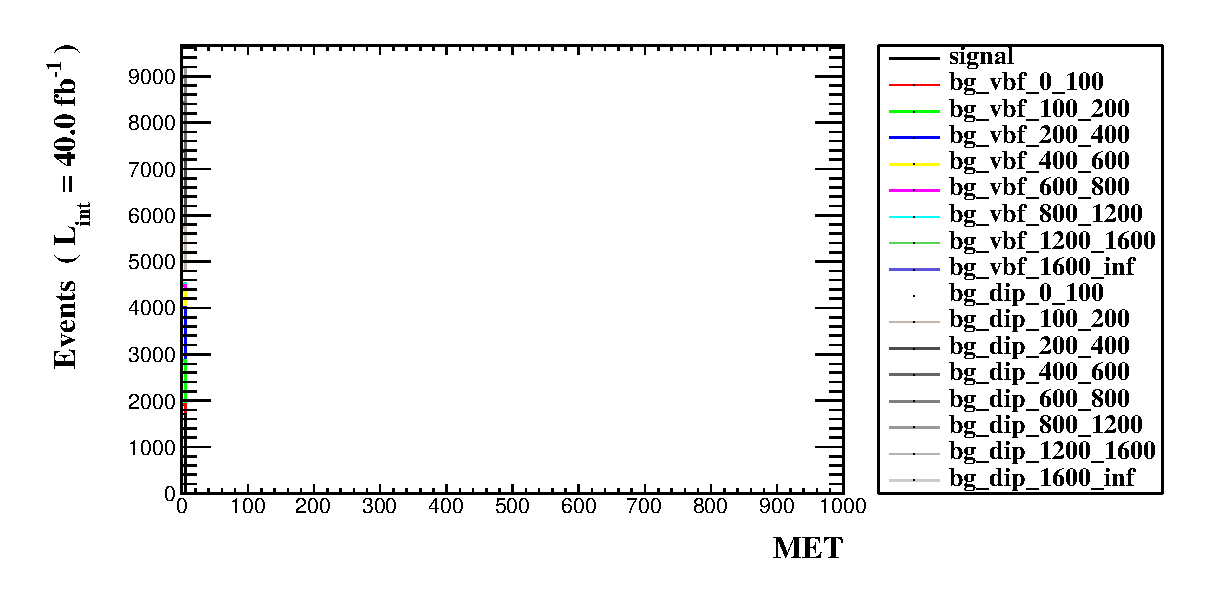
\includegraphics[scale=0.45]{selection_13.eps}\\
\caption{   }
  \end{center}
\end{figure}
      \newpage
\subsection{ Histogram 15}

\textbf{* Plot: TET}\\
   \begin{table}[H]
  \begin{center}
    \begin{tabular}{|m{23.0mm}|m{23.0mm}|m{18.0mm}|m{19.0mm}|m{19.0mm}|m{19.0mm}|m{19.0mm}|}
      \hline
      {\cellcolor{yellow}         Dataset}& {\cellcolor{yellow}         Integral}& {\cellcolor{yellow}         Entries per event}& {\cellcolor{yellow}         Mean}& {\cellcolor{yellow}         RMS}& {\cellcolor{yellow}         \% underflow}& {\cellcolor{yellow}         \% overflow}\\
      \hline
      {\cellcolor{white}         signal\_1pt8tevl}& {\cellcolor{white}         71.6}& {\cellcolor{white}         1.0}& {\cellcolor{white}         1796.63}& {\cellcolor{white}         802.7}& {\cellcolor{green}         0.0}& {\cellcolor{green}         0.0}\\
      \hline
      {\cellcolor{white}         signal\_2tevl}& {\cellcolor{white}         44.7}& {\cellcolor{white}         1.0}& {\cellcolor{white}         1786.93}& {\cellcolor{white}         803.4}& {\cellcolor{green}         0.0}& {\cellcolor{green}         0.002388}\\
      \hline
      {\cellcolor{white}         signal\_2pt2tevl}& {\cellcolor{white}         29.7}& {\cellcolor{white}         1.0}& {\cellcolor{white}         1778.31}& {\cellcolor{white}         807.7}& {\cellcolor{green}         0.0}& {\cellcolor{green}         0.002341}\\
      \hline
      {\cellcolor{white}         signal\_2pt4tevl}& {\cellcolor{white}         20.5}& {\cellcolor{white}         1.0}& {\cellcolor{white}         1771.36}& {\cellcolor{white}         814.1}& {\cellcolor{green}         0.0}& {\cellcolor{green}         0.0}\\
      \hline
      {\cellcolor{white}         bg\_dip\_0\_100}& {\cellcolor{white}         0.0 +/\-- 0.0}& {\cellcolor{white}         0.}& {\cellcolor{white}         0.0}& {\cellcolor{white}         0.0}& {\cellcolor{green}         0.0}& {\cellcolor{green}         0.0}\\
      \hline
      {\cellcolor{white}         bg\_dip\_100\_200}& {\cellcolor{white}         3.16}& {\cellcolor{white}         1.0}& {\cellcolor{white}         728.733}& {\cellcolor{white}         80.65}& {\cellcolor{green}         0.0}& {\cellcolor{green}         0.0}\\
      \hline
      {\cellcolor{white}         bg\_dip\_200\_400}& {\cellcolor{white}         25.8}& {\cellcolor{white}         1.0}& {\cellcolor{white}         914.659}& {\cellcolor{white}         167.9}& {\cellcolor{green}         0.0}& {\cellcolor{green}         0.0}\\
      \hline
      {\cellcolor{white}         bg\_dip\_400\_600}& {\cellcolor{white}         29.4}& {\cellcolor{white}         1.0}& {\cellcolor{white}         1086.07}& {\cellcolor{white}         197.0}& {\cellcolor{green}         0.0}& {\cellcolor{green}         0.0}\\
      \hline
      {\cellcolor{white}         bg\_dip\_600\_800}& {\cellcolor{white}         11.9}& {\cellcolor{white}         1.0}& {\cellcolor{white}         1379.01}& {\cellcolor{white}         239.6}& {\cellcolor{green}         0.0}& {\cellcolor{green}         0.0}\\
      \hline
      {\cellcolor{white}         bg\_dip\_800\_1200}& {\cellcolor{white}         6.14}& {\cellcolor{white}         1.0}& {\cellcolor{white}         1750.17}& {\cellcolor{white}         319.8}& {\cellcolor{green}         0.0}& {\cellcolor{green}         0.0}\\
      \hline
      {\cellcolor{white}         bg\_dip\_1200\_1600}& {\cellcolor{white}         0.83}& {\cellcolor{white}         1.0}& {\cellcolor{white}         2301.02}& {\cellcolor{white}         455.2}& {\cellcolor{green}         0.0}& {\cellcolor{green}         0.0}\\
      \hline
      {\cellcolor{white}         bg\_dip\_1600\_inf}& {\cellcolor{white}         0.132}& {\cellcolor{white}         1.0}& {\cellcolor{white}         2867.98}& {\cellcolor{white}         644.6}& {\cellcolor{green}         0.0}& {\cellcolor{green}         0.0}\\
      \hline
      {\cellcolor{white}         bg\_vbf\_0\_100}& {\cellcolor{white}         0.0486}& {\cellcolor{white}         1.0}& {\cellcolor{white}         814.434}& {\cellcolor{white}         141.3}& {\cellcolor{green}         0.0}& {\cellcolor{green}         0.0}\\
      \hline
      {\cellcolor{white}         bg\_vbf\_100\_200}& {\cellcolor{white}         1.16}& {\cellcolor{white}         1.0}& {\cellcolor{white}         822.463}& {\cellcolor{white}         164.7}& {\cellcolor{green}         0.0}& {\cellcolor{green}         0.0}\\
      \hline
      {\cellcolor{white}         bg\_vbf\_200\_400}& {\cellcolor{white}         6.68}& {\cellcolor{white}         1.0}& {\cellcolor{white}         911.682}& {\cellcolor{white}         196.9}& {\cellcolor{green}         0.0}& {\cellcolor{green}         0.0}\\
      \hline
      {\cellcolor{white}         bg\_vbf\_400\_600}& {\cellcolor{white}         6.68}& {\cellcolor{white}         1.0}& {\cellcolor{white}         1089.7}& {\cellcolor{white}         208.6}& {\cellcolor{green}         0.0}& {\cellcolor{green}         0.0}\\
      \hline
      {\cellcolor{white}         bg\_vbf\_600\_800}& {\cellcolor{white}         3.03}& {\cellcolor{white}         1.0}& {\cellcolor{white}         1357.34}& {\cellcolor{white}         214.2}& {\cellcolor{green}         0.0}& {\cellcolor{green}         0.0}\\
      \hline
      {\cellcolor{white}         bg\_vbf\_800\_1200}& {\cellcolor{white}         1.58}& {\cellcolor{white}         1.0}& {\cellcolor{white}         1735.73}& {\cellcolor{white}         292.6}& {\cellcolor{green}         0.0}& {\cellcolor{green}         0.0}\\
      \hline
      {\cellcolor{white}         bg\_vbf\_1200\_1600}& {\cellcolor{white}         0.236}& {\cellcolor{white}         1.0}& {\cellcolor{white}         2307.64}& {\cellcolor{white}         386.5}& {\cellcolor{green}         0.0}& {\cellcolor{green}         0.0}\\
      \hline
      {\cellcolor{white}         bg\_vbf\_1600\_inf}& {\cellcolor{white}         0.0444}& {\cellcolor{white}         1.0}& {\cellcolor{white}         2955.83}& {\cellcolor{white}         592.9}& {\cellcolor{green}         0.0}& {\cellcolor{green}         0.0}\\
\hline
    \end{tabular}
  \end{center}
\end{table}

\begin{figure}[H]
  \begin{center}
    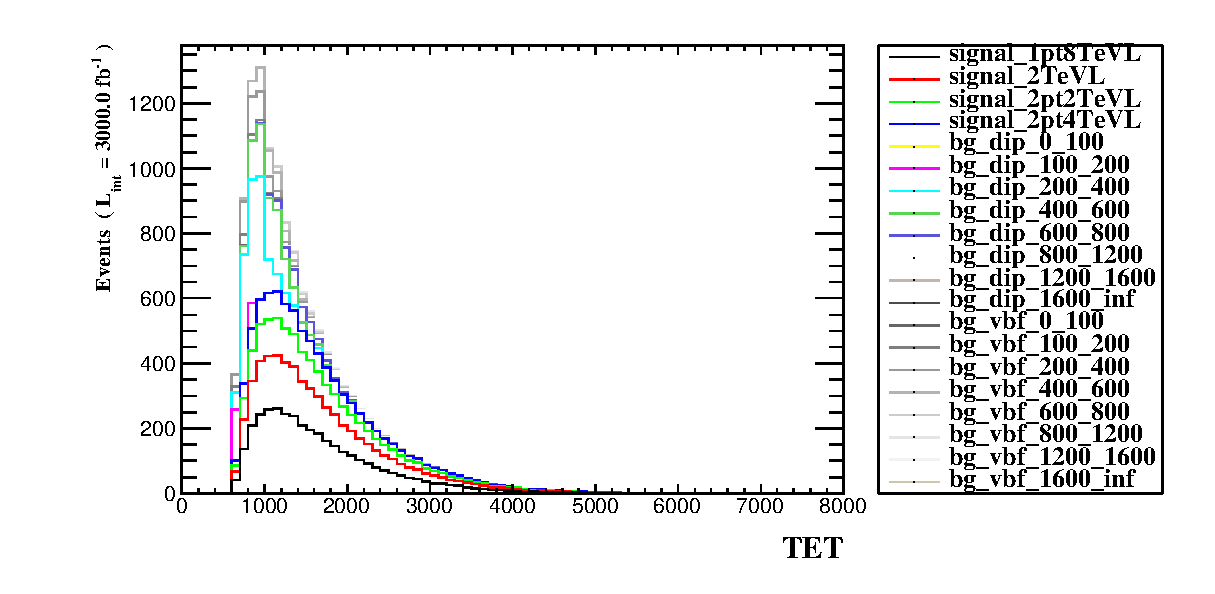
\includegraphics[scale=0.45]{selection_14.eps}\\
\caption{   }
  \end{center}
\end{figure}
      % -----------------------------------------------------------------------------
%                                SECTION Summary                                
% -----------------------------------------------------------------------------
\newpage
\section{ Summary}

\subsection{Cut-flow charts}

\begin{itemize}
  \item How to compare signal (S) and background (B): \textcolor{blue}{S/\-sqrt(S+B+(xB)**2)} .
   \item Object definition selections are indicated in cyan.  \item Reject and select are indicated by 'REJ' and 'SEL' respectively
\end{itemize}
\begin{table}[H]
  \begin{center}
    \begin{tabular}{|m{36.0mm}|m{36.0mm}|m{36.0mm}|m{33.0mm}|}
      \hline
      {\cellcolor{yellow}        Cuts}& {\cellcolor{yellow}         Signal (S)}& {\cellcolor{yellow}         Background (B)}& {\cellcolor{yellow}         S vs B}\\
      \hline
      {\cellcolor{white}         Initial (no cut)}& {\cellcolor{white}         400.622 +/\-- 0.237}& {\cellcolor{white}         4113516 +/\-- 4877}& {\cellcolor{white}         3.90e-04 +/\-- 2.58e-07}\\
      \hline
      {\cellcolor{white} SEL: ( ( sdETA ( jets[1] jets[2] ) > 2.6 or sdETA }& {\cellcolor{white}         165.82 +/\-- 9.86}& {\cellcolor{white}         96.80 +/\-- 9.83}& {\cellcolor{white}         5.694 +/\-- 0.356}\\
\hline
    \end{tabular}
  \end{center}
\end{table}

\end{document}
